\chapter{Definición del instrumento}
\minitoc

Una vez definidos los fundamentos teóricos que rigen el problema planteado en el presente trabajo, se comienza a definir las variables que cumplan los requisitos impuestos.

Se ha creado para el trabajo un paquete de códigos disponible en el anexo \ref{sec:annexcode} que, en base a los \textit{inputs} iniciales, calcula los requerimientos y exporta las soluciones óptimas listas a interpretar por el usuario. El código maestro, que aloja dichos parámetros de entrada y las llamadas a las funciones, alberga el siguiente flujo de trabajo:

\begin{landscape}
    

\begin{figure}[H]
    \centering
    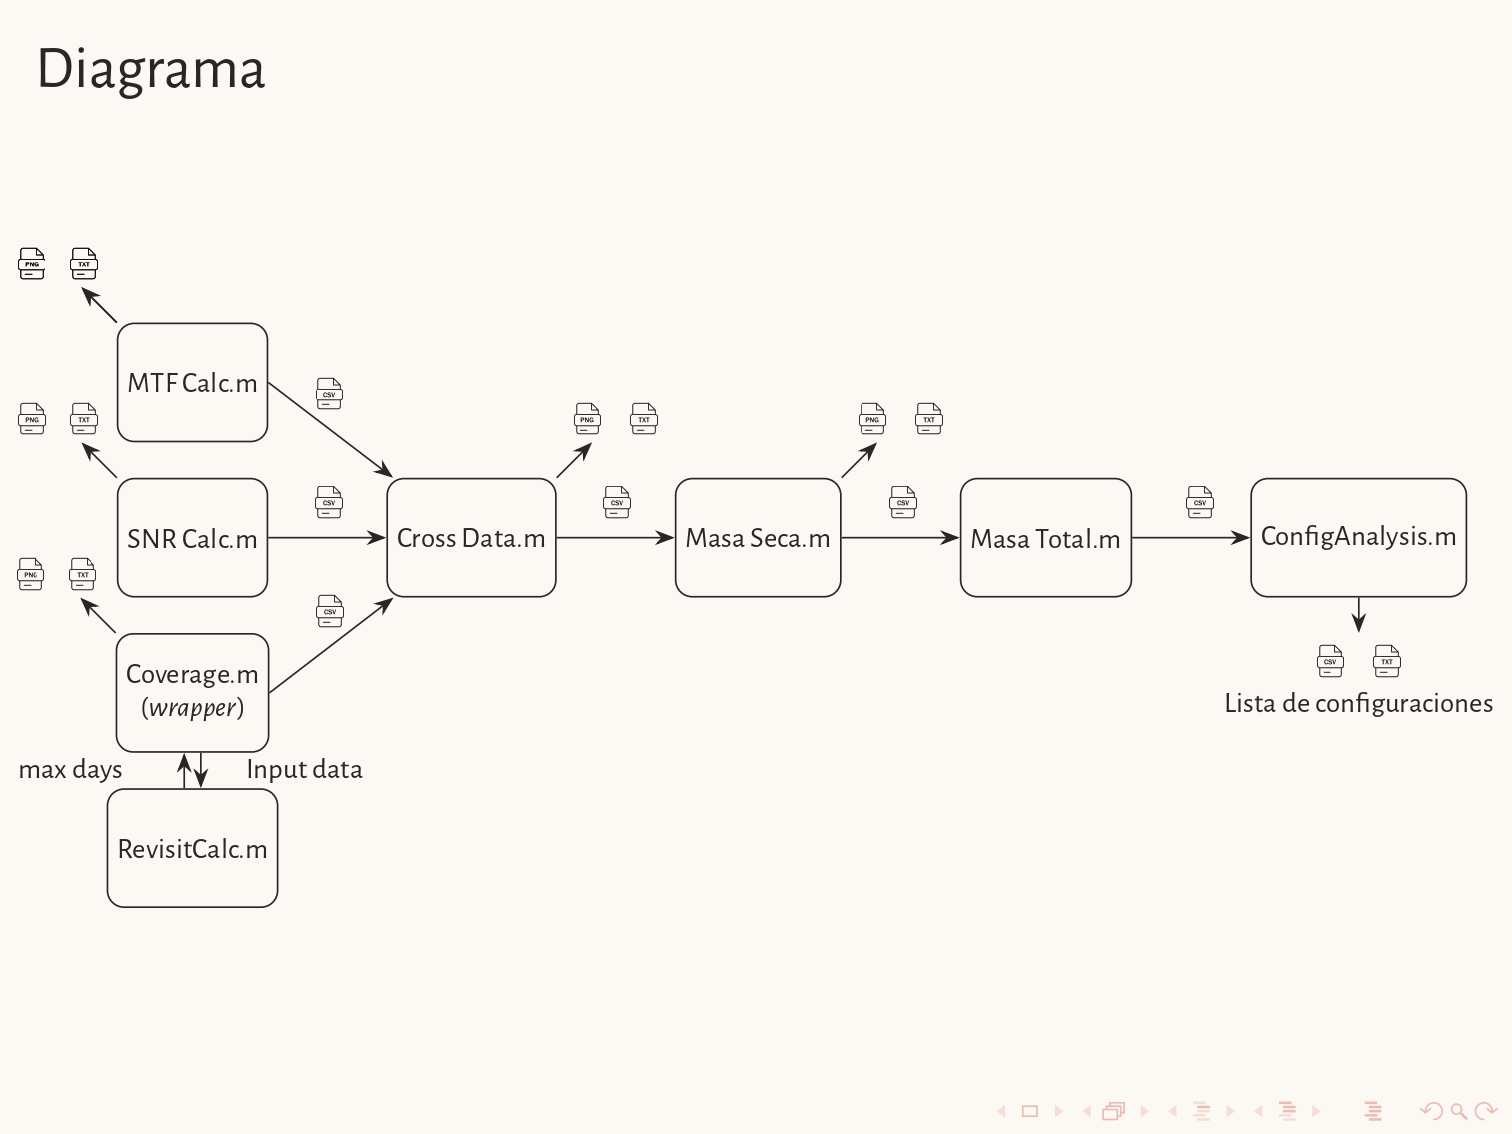
\includegraphics[width=1\linewidth]{4.Payload/workflow.jpg}
    \caption{Flujo de trabajo de los scripts de MATLAB}
    \label{fig:flowchart}
\end{figure}
\end{landscape}
\newpage

\section{GSD}

Se comenzará por definir el GSD, ya que es un parámetro que implícitamente viene dado por las condiciones del cliente. Según el requerimiento debemos ser capaces de poder diferenciar fuentes puntuales de CO2 en las ciudades estadounidenses.

Primeramente se extrae una imagen satélite del cinturón industrial de Houston para escoger de una manera mas visual la selección de GSD. Mediante el software \textit{open source} GIMP se puede pixelar esta imagen para visualizar la elección del GSD. Dicha foto tiene 1673 pixeles de ancho, y mediante el software Google Earth, proporciona el dato del ancho de la imagen en la realidad, correspondiente a 14251 m. Por tanto, el GSD de esta captura será: 

\begin{equation}
\frac{14251\ m}{1673\ pix} \approx 8.516
\end{equation}


\begin{figure}[H]
    \centering
    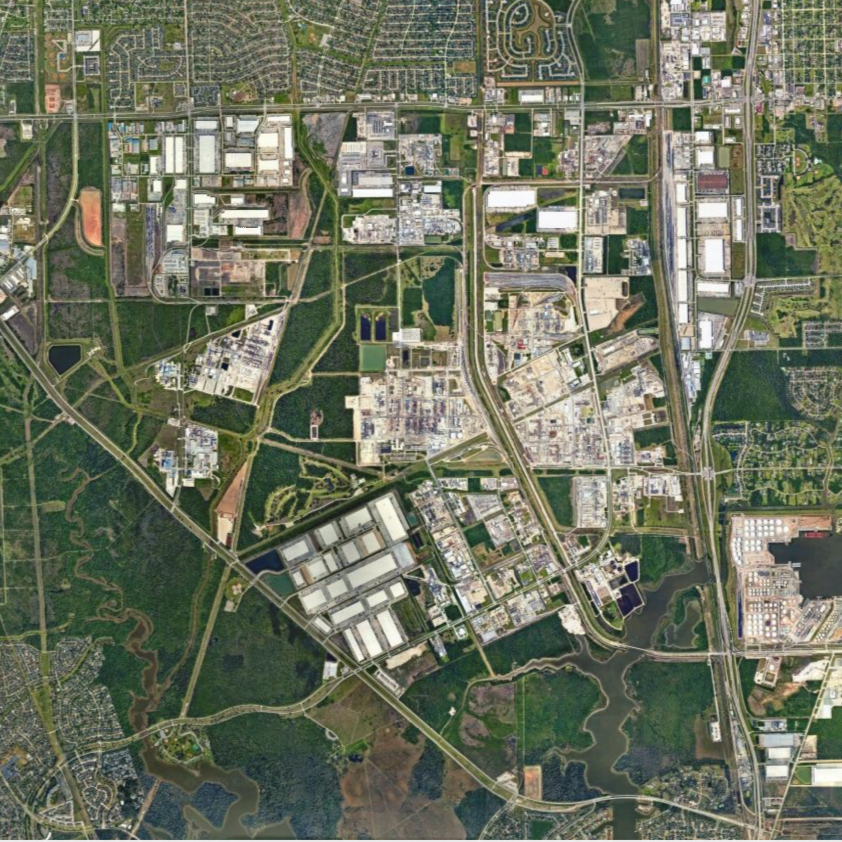
\includegraphics[width=0.7\textwidth]{4.Payload/Houston.jpg}
    \caption{Imagen satélite del cinturón industrial de Houston. $GSD \approx 8,5$. \\ Fuente: Google Earth (29°42'18.0"N; 95°00'10.8"W)}
    \label{fig:Houston}
\end{figure}

Esta resolución resulta excesiva para las especificaciones del proyecto, ya que permite observar las instalaciones industriales con gran detalle. Se puede sacrificar este parámetro en favor del resto de variables a seleccionar. Un análisis comparativo con diferentes valores de GSD demuestra que una resolución de \textbf{80 metros} permite diferenciar edificios industriales entre sí y distinguirlos de las zonas residenciales, cumpliendo así con los requerimientos de precisión del cliente.

\begin{figure}[H]
    \centering

    % Primera fila
    \begin{subfigure}[b]{0.3\textwidth}
        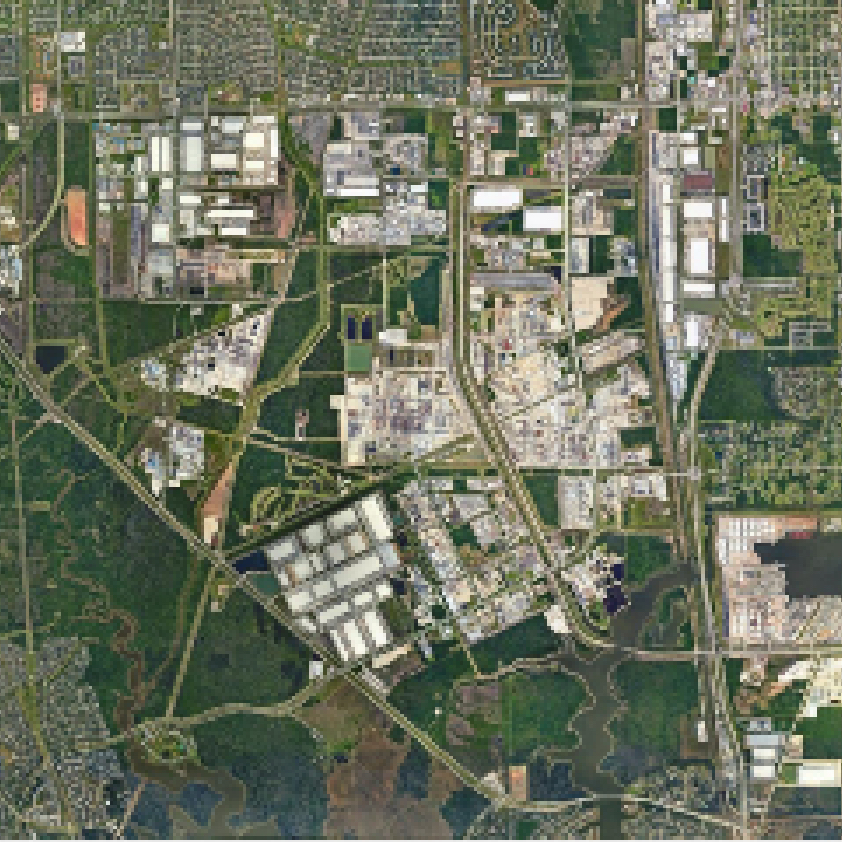
\includegraphics[width=\textwidth]{4.Payload/Houston GSD 30.jpg}
        \subcaption{GSD 30}
    \end{subfigure}
    \hfill
    \begin{subfigure}[b]{0.3\textwidth}
        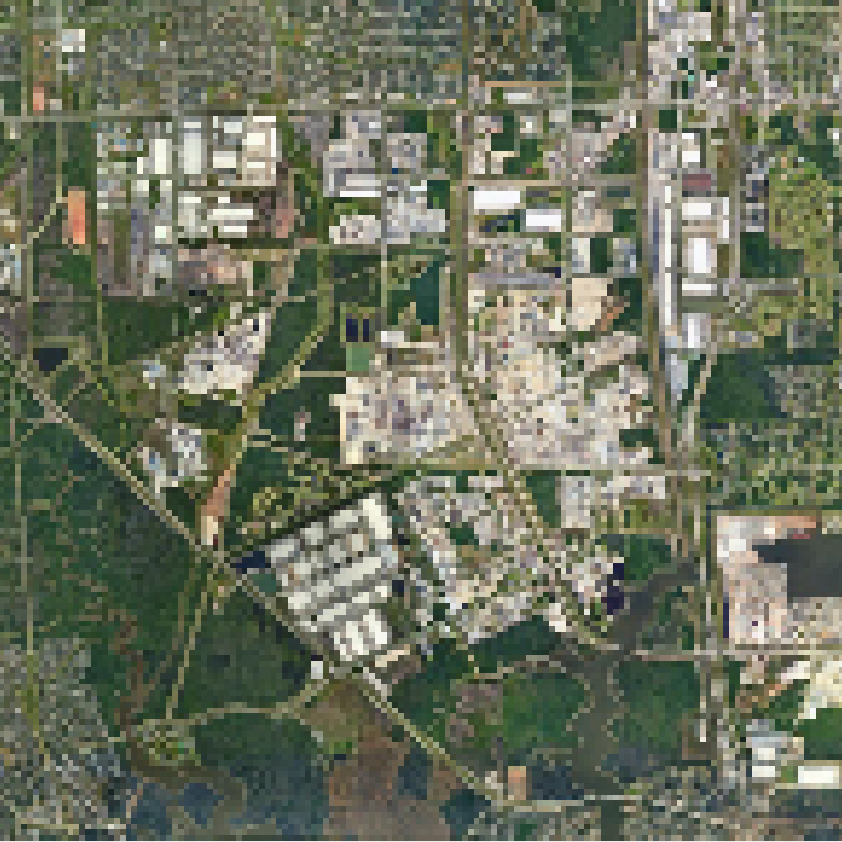
\includegraphics[width=\textwidth]{4.Payload/HoustonGSD50.jpg}
        \subcaption{GSD 50}
    \end{subfigure}
    \hfill
    \begin{subfigure}[b]{0.3\textwidth}
        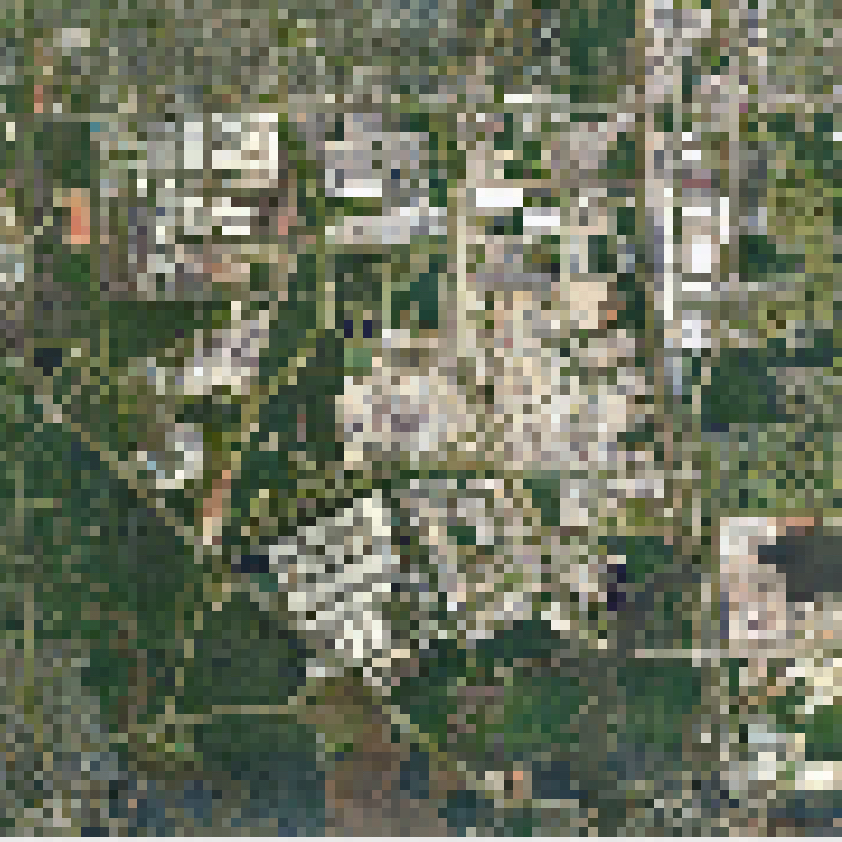
\includegraphics[width=\textwidth]{4.Payload/HoustonGSD80.jpg}
        \subcaption{GSD 80}
    \end{subfigure}

    \vspace{1em}

    % Segunda fila
    \begin{subfigure}[b]{0.3\textwidth}
        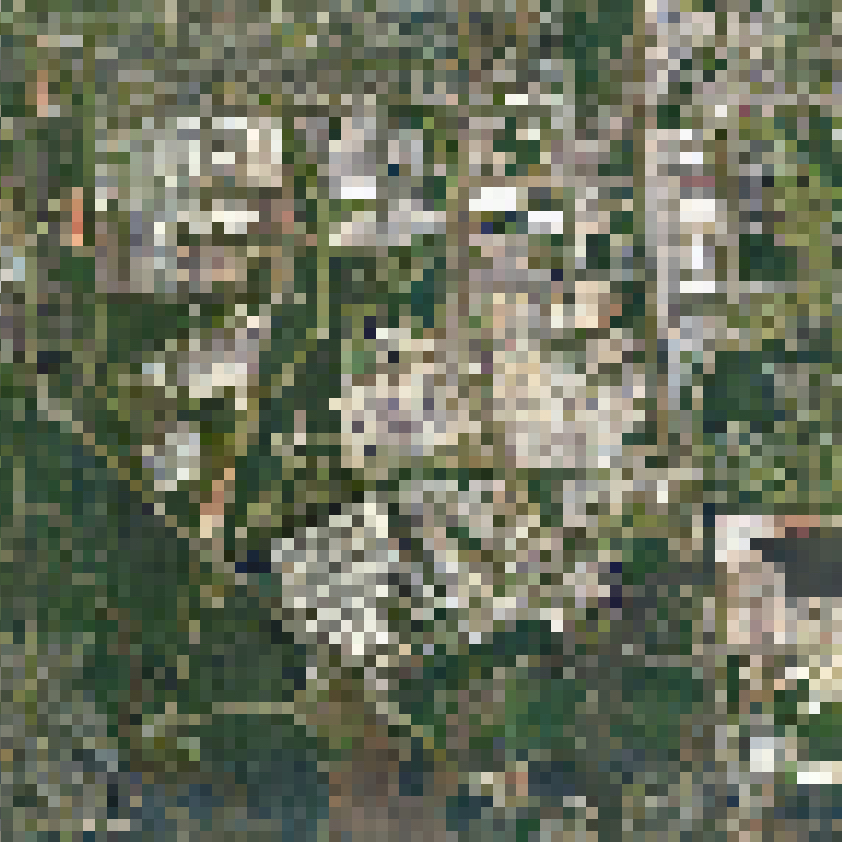
\includegraphics[width=\textwidth]{4.Payload/HoustonGSD100.jpg}
        \subcaption{GSD 100}
    \end{subfigure}
    \hfill
    \begin{subfigure}[b]{0.3\textwidth}
        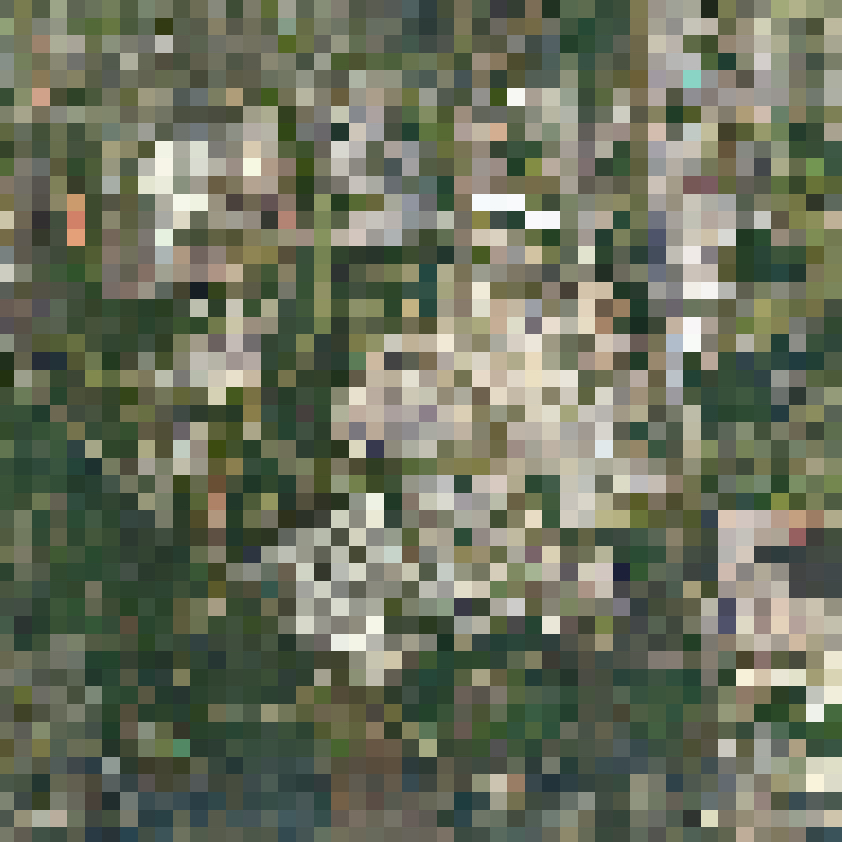
\includegraphics[width=\textwidth]{4.Payload/Houston GSD150.jpg}
        \subcaption{GSD 150}
    \end{subfigure}
    \hfill
    \begin{subfigure}[b]{0.3\textwidth}
        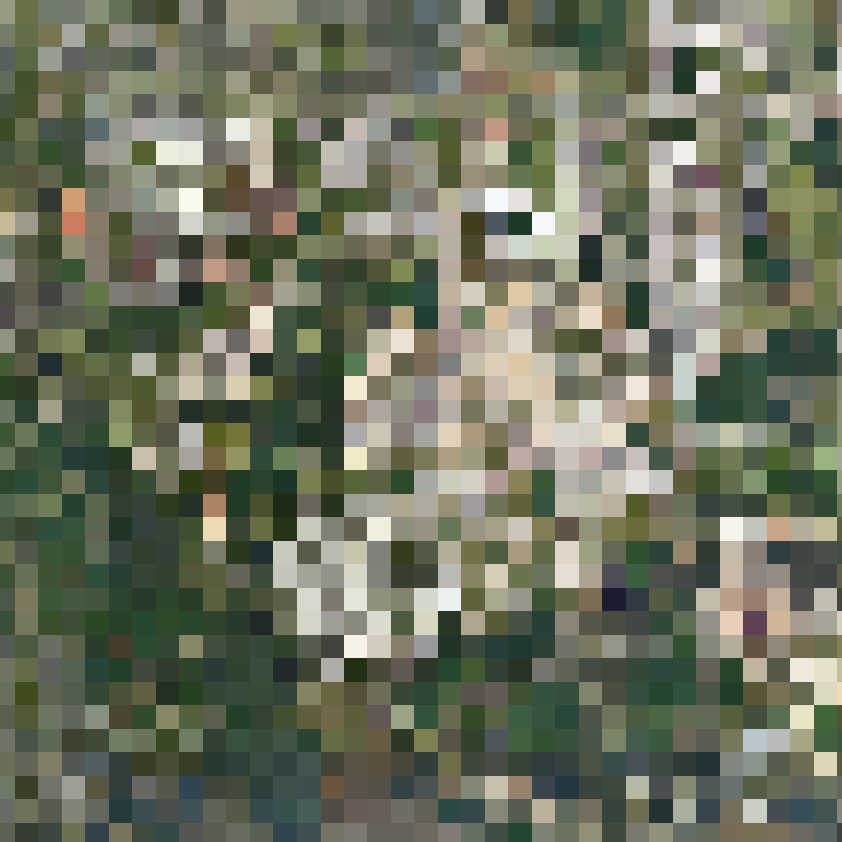
\includegraphics[width=\textwidth]{4.Payload/Houston GSD200.jpg}
        \subcaption{GSD 200}
    \end{subfigure}

    \caption{Comparación de imágenes con distintas condiciones de GSD. \\Fuente: Imagen adaptada, Google Earth.}
    \label{fig:comparacion_gsd}
\end{figure}


\section{Bandas espectrales. Ancho de banda} \label{sec:specbands}

La selección de bandas espectrales se fundamenta en las características de absorción del CO\textsubscript{2} y los requisitos de calibración atmosférica necesarios para garantizar la precisión de las mediciones.

\subsubsection{Banda O\textsubscript{2} A-Band (0,76 \textmu m)}

La banda de absorción del oxígeno atmosférico a 0,76 \textmu m se emplea para la calibración de la columna de aire. El oxígeno presenta una concentración atmosférica estable y conocida (20,95\%), lo que permite determinar con precisión la masa de aire atravesada por la radiación solar. Esta referencia resulta esencial para normalizar las mediciones de CO\textsubscript{2} y corregir variaciones debidas a diferencias en el camino óptico atmosférico.

\subsubsection{Bandas CO\textsubscript{2} SWIR (1,61 y 2,06 \textmu m)}

Las bandas de 1610 nm y 2060 nm corresponden a las principales regiones de absorción del CO\textsubscript{2} en el infrarrojo de onda corta, como se vio en el capítulo \ref{cap3}. La utilización de dos bandas independientes permite implementar algoritmos de validación cruzada y mejora el calculo de estimaciones de concentración.

\subsubsection{Ancho de banda}

En cuanto al ancho de banda espectral, se ha seleccionado un valor de 20 nm para todas las bandas. Esta elección representa un equilibrio entre la resolución espectral y la relación señal-ruido, permitiendo aislar adecuadamente las características de absorción objetivo sin comprometer la sensibilidad del sistema. Un ancho de banda más estrecho proporcionaría mayor especificidad espectral, pero reduciría la cantidad de fotones detectados y, por tanto, la SNR. Por el contrario, un ancho de banda excesivamente amplio dificultaría la discriminación de las líneas de absorción. El valor adoptado se encuentra dentro de los estándares habituales en instrumentación óptica para aplicaciones de teledetección y garantiza el cumplimiento de los requisitos de precisión y robustez en la recuperación de concentraciones de CO\textsubscript{2} y parámetros atmosféricos \cite{skoog2017principles,}.
\\

\begin{table}[h]
\centering
\caption{Bandas espectrales elegidas.}
\begin{tabular}{l c c l}
\toprule
\textbf{Banda} & \textbf{$\lambda$ (\textmu m)} & \textbf{$\Delta\lambda$ (nm)} & \textbf{Propósito principal} \\
\midrule
O$_2$ A-Band       & 0,76  & 20    & Calibración columna aire \\
CO$_2$ SWIR 1      & 1,61  & 20    & Absorción principal de CO$_2$ \\
CO$_2$ SWIR 2      & 2,06  & 20    & Absorción secundaria de CO$_2$ \\
\bottomrule
\end{tabular}

\label{tab:banda_propósitos}
\end{table}



\section{Detectores, filtros y escaneo}



\subsection{Elección de detectores}

Una vez definidas las bandas de interés se procederá a buscar el detector que sea capaz de cubrir dichos rangos de detección para la misión. Para ello, se elabora una lista de detectores disponibles en mercado de los cuales se escogerán mas adelante, el más apropiado según sus especificaciones. Para las bandas 1,61 \textmu m y 2,01 \textmu m se evaluaran los siguientes detectores:

%% TABLA
\begin{table}[H]
\centering
\caption{Comparación de características de detectores SWIR}
\begin{tabular}{lccc}
\toprule
& \textbf{Detector 1} \cite{lynred_capyork} & \textbf{Detector 2} \cite{teledyne_hawaii2rg} & \textbf{Detector 3} \cite{sofradir_saturn_visir_2011}\\
\midrule
\textbf{Nombre} & LYNRED CAPYORK  & Teledyne H2RG   & Saturn VISIR \\
\textbf{Tamaño pixel} & 15 x 15 \textmu m & 18 × 18 \textmu m & 30 × 30 \textmu m \\
\textbf{Array} & 1200 × 12 & 2048 × 2048 &  1000 × 256 \\
\textbf{Canales\tablefootnote{Evaluar los canales de salida permite evaluar cuantas bandas independientes es capaz de capturar un detector}} & 4 & 4 & 4 ó 8 \\
\textbf{TDI} & Si (4 etapas) & No  & No \\
\textbf{Rango espectral} & 0,8-5 \textmu m & 0,4-2,5 \textmu m & 0,3-2,5 \textmu m \\
\textbf{Eficiencia cuántica} & 85\% &  70\% &  70\%  \\
\textbf{MTF @ Nyquist} & 0,45  & 0,5 & 0,48 \\
\bottomrule
\end{tabular}

\label{tab:detectores_comparacion}
\end{table}

Se aprecia que los detectores 2 y 3 tienen un rango válido para evaluarse también en la banda 0,76 \textmu m, mientras que el Detector CAPYORK será incapaz de recepcionar datos en esta banda. Por ello, para la banda O\textsubscript{2} se evaluarán, además de los detectores 2 y 3, un detector adicional que complemente al LYNRED CAPYORK. Resulta el CMOS STAR250 una opción a evaluar: 

%% TABLA

\begin{table}[H]
\centering
\caption{Comparación de características de detectores para \textit{A-Band} O\textsubscript{2}.}
\label{tab:detectores_comparacion_2}
\begin{tabular}{lccc}
\toprule
& \textbf{Detector 4} \cite{cypress_star250_2009}  & \textbf{Detector 5}\cite{teledyne_hawaii2rg} & \textbf{Detector 6} \cite{sofradir_saturn_visir_2011} \\
\midrule
\textbf{Nombre} & STAR250 & Teledyne H2RG & SATURN VISIR \\
\textbf{Tamaño pixel} & 25 × 25 \textmu m & 18 × 18 \textmu m & 30 × 30 \textmu m \\
\textbf{Array} & 512 × 512 & 2048 × 2048 & 1000 × 256 \\
\textbf{Canales} & 4 & 4 & 4 ó 8 \\
\textbf{TDI} & No & No  & No  \\
\textbf{Rango espectral} & 0,4–1,1 \textmu m & 0,4–2,5 \textmu m & 0,3 –2,5 \textmu m \\
\textbf{Eficiencia cuántica} & 35 \% &  70\% &  50\% \tablefootnote{Según especificaciones del fabricante; desciende un 20\% para rango visible} \\
\textbf{MTF @ Nyquist} & 0,36 & 0,5 & 0,45 \\
\bottomrule
\end{tabular}

\end{table}


Más adelante se determinará el número de detectores a utilizar, así como su disposición, ya que se debe trabajar con un \textit{swath} mínimo para asegurar cobertura.


\subsection{Método de escaneo}

El escaneo \textbf{\textit{pushbroom}} se elige sobre alternativas como \textit{whiskbroom} o \textit{step and stare} por su fiabilidad, simplicidad mecánica y optimización de la relación señal-ruido. A diferencia del \textit{whiskbroom}, que utiliza espejos oscilantes para barrer transversalmente la franja de observación, el \textit{pushbroom} emplea un array lineal de detectores fijos que captura toda la franja simultáneamente. Esto elimina componentes mecánicos, reduce el riesgo de desgaste y simplifica el diseño.

Además, el \textit{pushbroom} ofrece un mayor tiempo de integración por píxel, lo que incrementa la SNR al permitir que los detectores acumulen más fotones. En comparación, el \textit{step and stare} limita la cobertura continua y exige maniobras satelitales complejas, añadiendo dificultad a las operaciones de mantenimiento en orbita, incrementando el peso para el control de actitud y limitando el tiempo de revisita.

\subsection{Eleccion de filtros}

Se escogen filtros \textit{\textbf{microstrip}} integrados en el mismo detector. La principal ventaja de los filtros microstrip frente a alternativas como la rueda de filtros reside en su baja masa y fiabilidad mecánica, ya que carecen completamente de partes móviles que pudieran fallar durante los 8 años de misión. Esta característica es crucial considerando el entorno espacial con sus ciclos térmicos extremos y vibraciones durante el lanzamiento. Además, permiten la adquisición simultánea de todas las bandas espectrales necesarias, lo que resulta fundamental para asegurar la correcta corregistración espacial de los datos.


Desde el punto de vista óptico, los filtros microstrip pueden optimizarse individualmente para cada banda espectral, permitiendo un ajuste fino del ancho de banda.


La implementación práctica implicaría fabricar filtros de interferencia multicapa específicamente diseñados para cada banda y detector, con materiales optimizados según el rango espectral (dieléctricos para visible/NIR, y compuestos especiales para SWIR). Estos se montarían directamente sobre cada array de detectores, lo que también minimiza el tamaño del instrumento al evitar mecanismos adicionales \cite{macleod2010}.

\section{Tipo de órbita. Altura orbital. Hora de paso local}

Como se ha expuesto en el capítulo \ref{semejantes}, las misiones de observación terrestre con requerimientos comparables adoptan, de manera unánime, \textbf{órbitas heliosíncronas}. Esta elección responde a la necesidad de garantizar condiciones de iluminación solar consistentes, ya que los detectores empleados dependen de la radiación solar para captar adecuadamente la señal reflejada desde la superficie terrestre.


Una limitación inherente a estos sistemas es su incapacidad para operar eficazmente en condiciones de penumbra. Por tanto, resulta esencial que la trayectoria orbital proporcione una iluminación solar directa y estable en cada pasada del satélite. La órbita heliosíncrona cumple precisamente este requisito, ya que su precesión mantiene el ángulo entre el plano orbital y el Sol constante a lo largo del año, asegurando que cada observación sobre una misma región se realice a una hora solar local fija. Esta estabilidad favorece la coherencia radiométrica de las imágenes y mejora la comparabilidad temporal de los datos adquiridos. Por ello se computarán soluciones de órbita \textbf{heliosíncrona entre los 350 km y los 1400 km de altitud}, con un discretización de 10 km de paso \cite{nasa_sso_slots_2011}.

Otras opciones de órbita compatibles con el requerimiento de iluminación podrían ser órbitas geoestacionarias o una constelación en orbitas Molniya. Estas no son consideradas en el trabajo, pues las alturas necesarias para este tipo de configuración orbital obliga a instalar diámetros de pupila mucho mayores a las requeridas en satélites en órbita LEO, aumentando el peso, el delta-V requerido para la inyección y por ende, el coste total de la misión.

Para la presente misión se ha seleccionado una \textbf{hora de paso ascendente local (LTAN) de 06:00}, lo que proporciona una configuración \textit{Dawn-Dusk}. En este tipo de órbita, el satélite cruza el ecuador terrestre cerca de la línea del línea crepuscular, donde la transición entre el día y la noche es continua. Esta disposición asegura que el satélite permanezca próximo al límite entre la zona iluminada y la zona en sombra de la Tierra, evitando así la entrada en el cono de sombra terrestre y garantizando la exposición solar durante toda la órbita. Como resultado, se obtienen condiciones de iluminación homogéneas tanto en las pasadas ascendentes como en las descendentes, maximizando las pasadas útiles\cite{Boain2004}.

\section{Cálculo de la MTF}

Con la base teórica definida en al apartado \ref{sec:MTFteoria}, así como las especificaciones de los detectores y telescopios a evaluar, se procede a computar en función de la altura orbital y el diámetro de pupila, mediante un script de MATLAB, los valores de MTF totales de la instrumentación óptica. La discretización del diámetro de pupila será de un paso de 1 mm.

Los valores a usar para la computación son:

\begin{table}[H]
\centering
\caption{Parámetros iniciales para el calculo de MTF. \\ Fuente: \cite{zorita_mtf_2023}.}
\begin{tabular}{l r}
\hline
\textbf{Parámetro} & \textbf{Valor} \\
\hline
MTF aberraciones & 0,95 \\
MTF fabricación & 0,98 \\
MTF vibraciones & 0,99 \\
MTF termoelástico & 0,95 \\
MTF Margen & 10\% \\
\hline
\end{tabular}

\end{table}

Dado que el proyecto se encuentra en una etapa temprana de diseño, se establece un margen del 10\% en el cálculo con el fin de cubrir posibles desviaciones asociadas a incertidumbres en los parámetros de entrada, tolerancias de fabricación, o variaciones operacionales. Este margen permite mantener una estimación conservadora sin comprometer la viabilidad preliminar del sistema.

Mediante un análisis dimensional, puede demostrarse que la función de transferencia de modulación (MTF, por sus siglas en inglés) es inversamente proporcional a la longitud de onda $\lambda$. Al aumentar $\lambda$, disminuye la frecuencia de corte $f_{co}$ y, en consecuencia, la capacidad del sistema para transmitir detalles de alta frecuencia espacial se ve reducida.

Por lo tanto, la banda más restrictiva corresponde a la mayor longitud de onda considerada. En el presente caso, para $\lambda = 2{,}01\,\mu\text{m}$, se obtiene la frecuencia de corte más baja y, por ende, la MTF más limitada, con lo que solo se presentan los datos de dicha banda. El resto de los datos se pueden encontrar en el anexo A. Así, junto con los valores de MTF de los detectores en la tabla \ref{tab:detectores_comparacion} y los valores de MTF de alineamiento de los telescopios de la tabla \ref{tab:tabla_telescopios}, se obtienen los siguientes resultados:

%% TABLAS MTF

%% Lambda 2
\begin{landscape}
\begin{figure}[p]
\centering
\setlength{\tabcolsep}{2pt}
\renewcommand{\arraystretch}{0}

\begin{tabular}{cc}
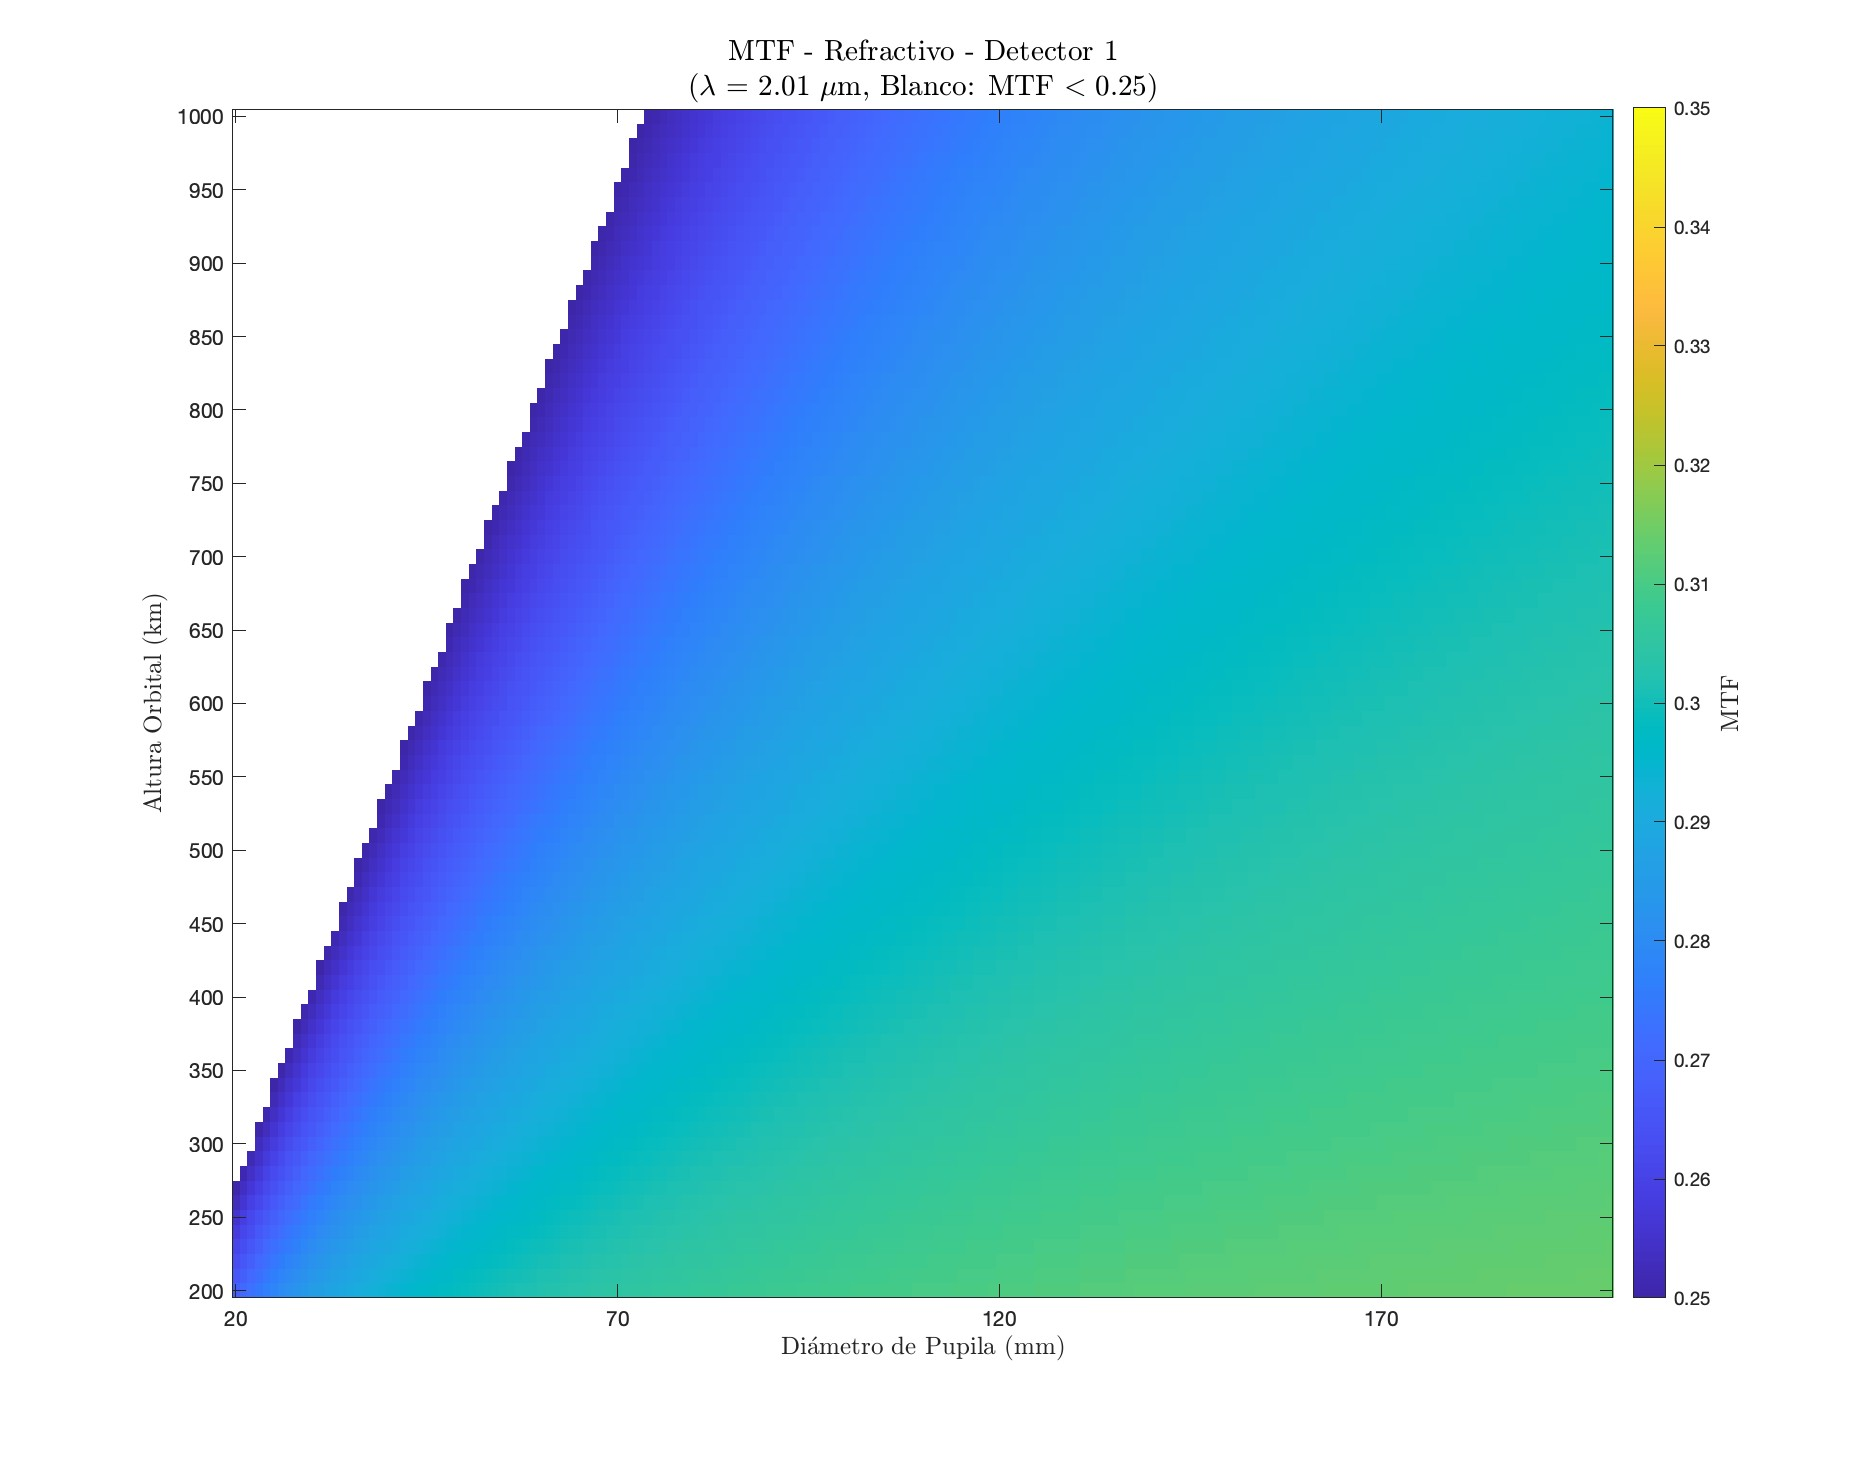
\includegraphics[width=0.48\linewidth]{4.Payload/MTF/MTF_Lambda2_Detector1_Telescopio1_heatmap.jpg} &
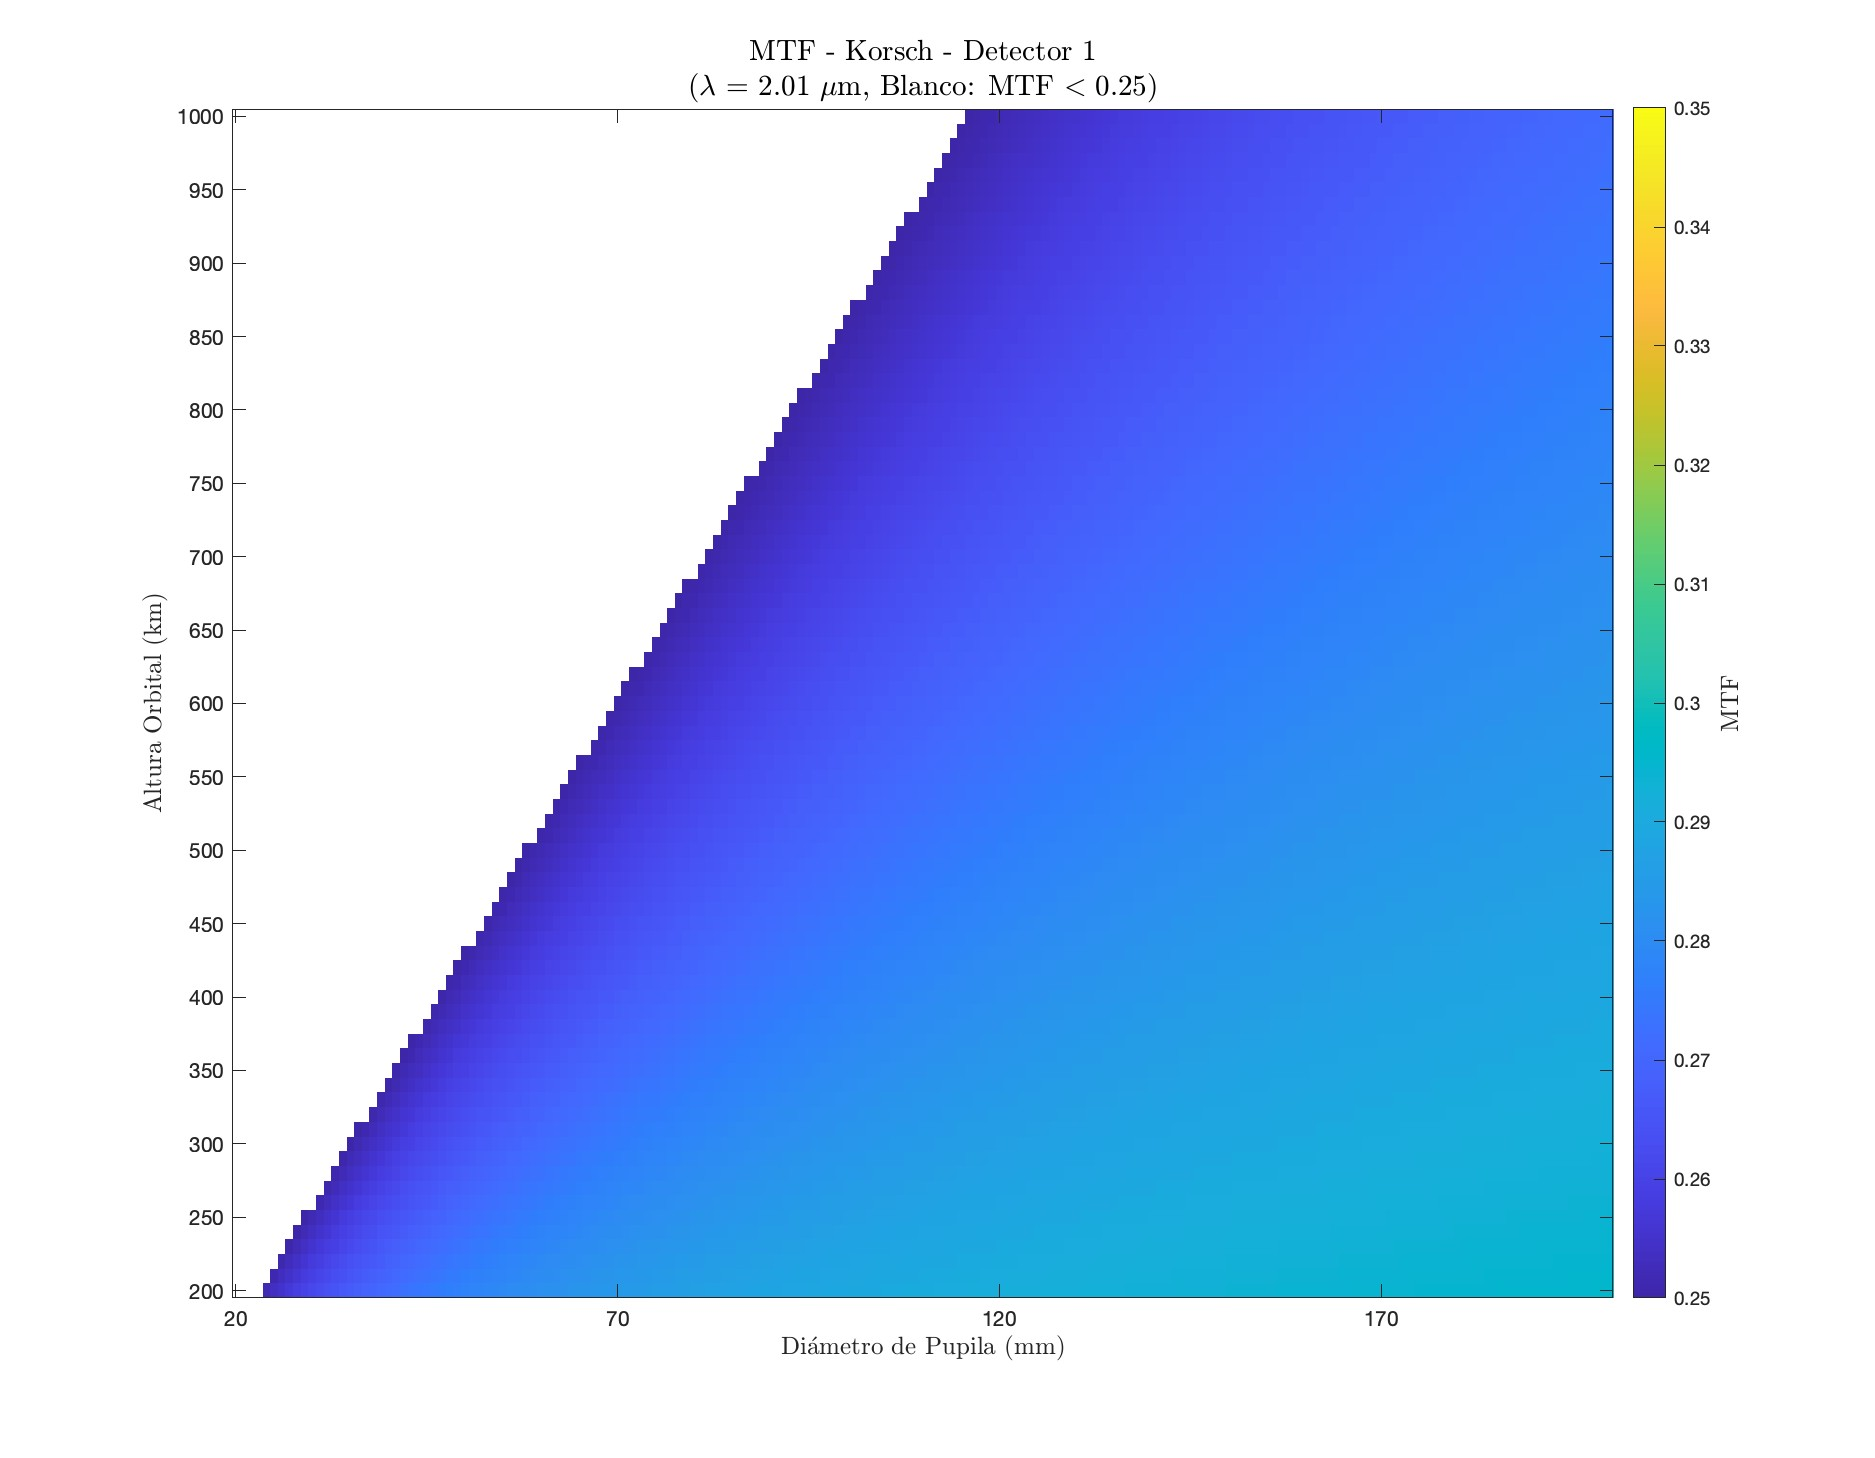
\includegraphics[width=0.48\linewidth]{4.Payload/MTF/MTF_Lambda2_Detector1_Telescopio2_heatmap.jpg} \\
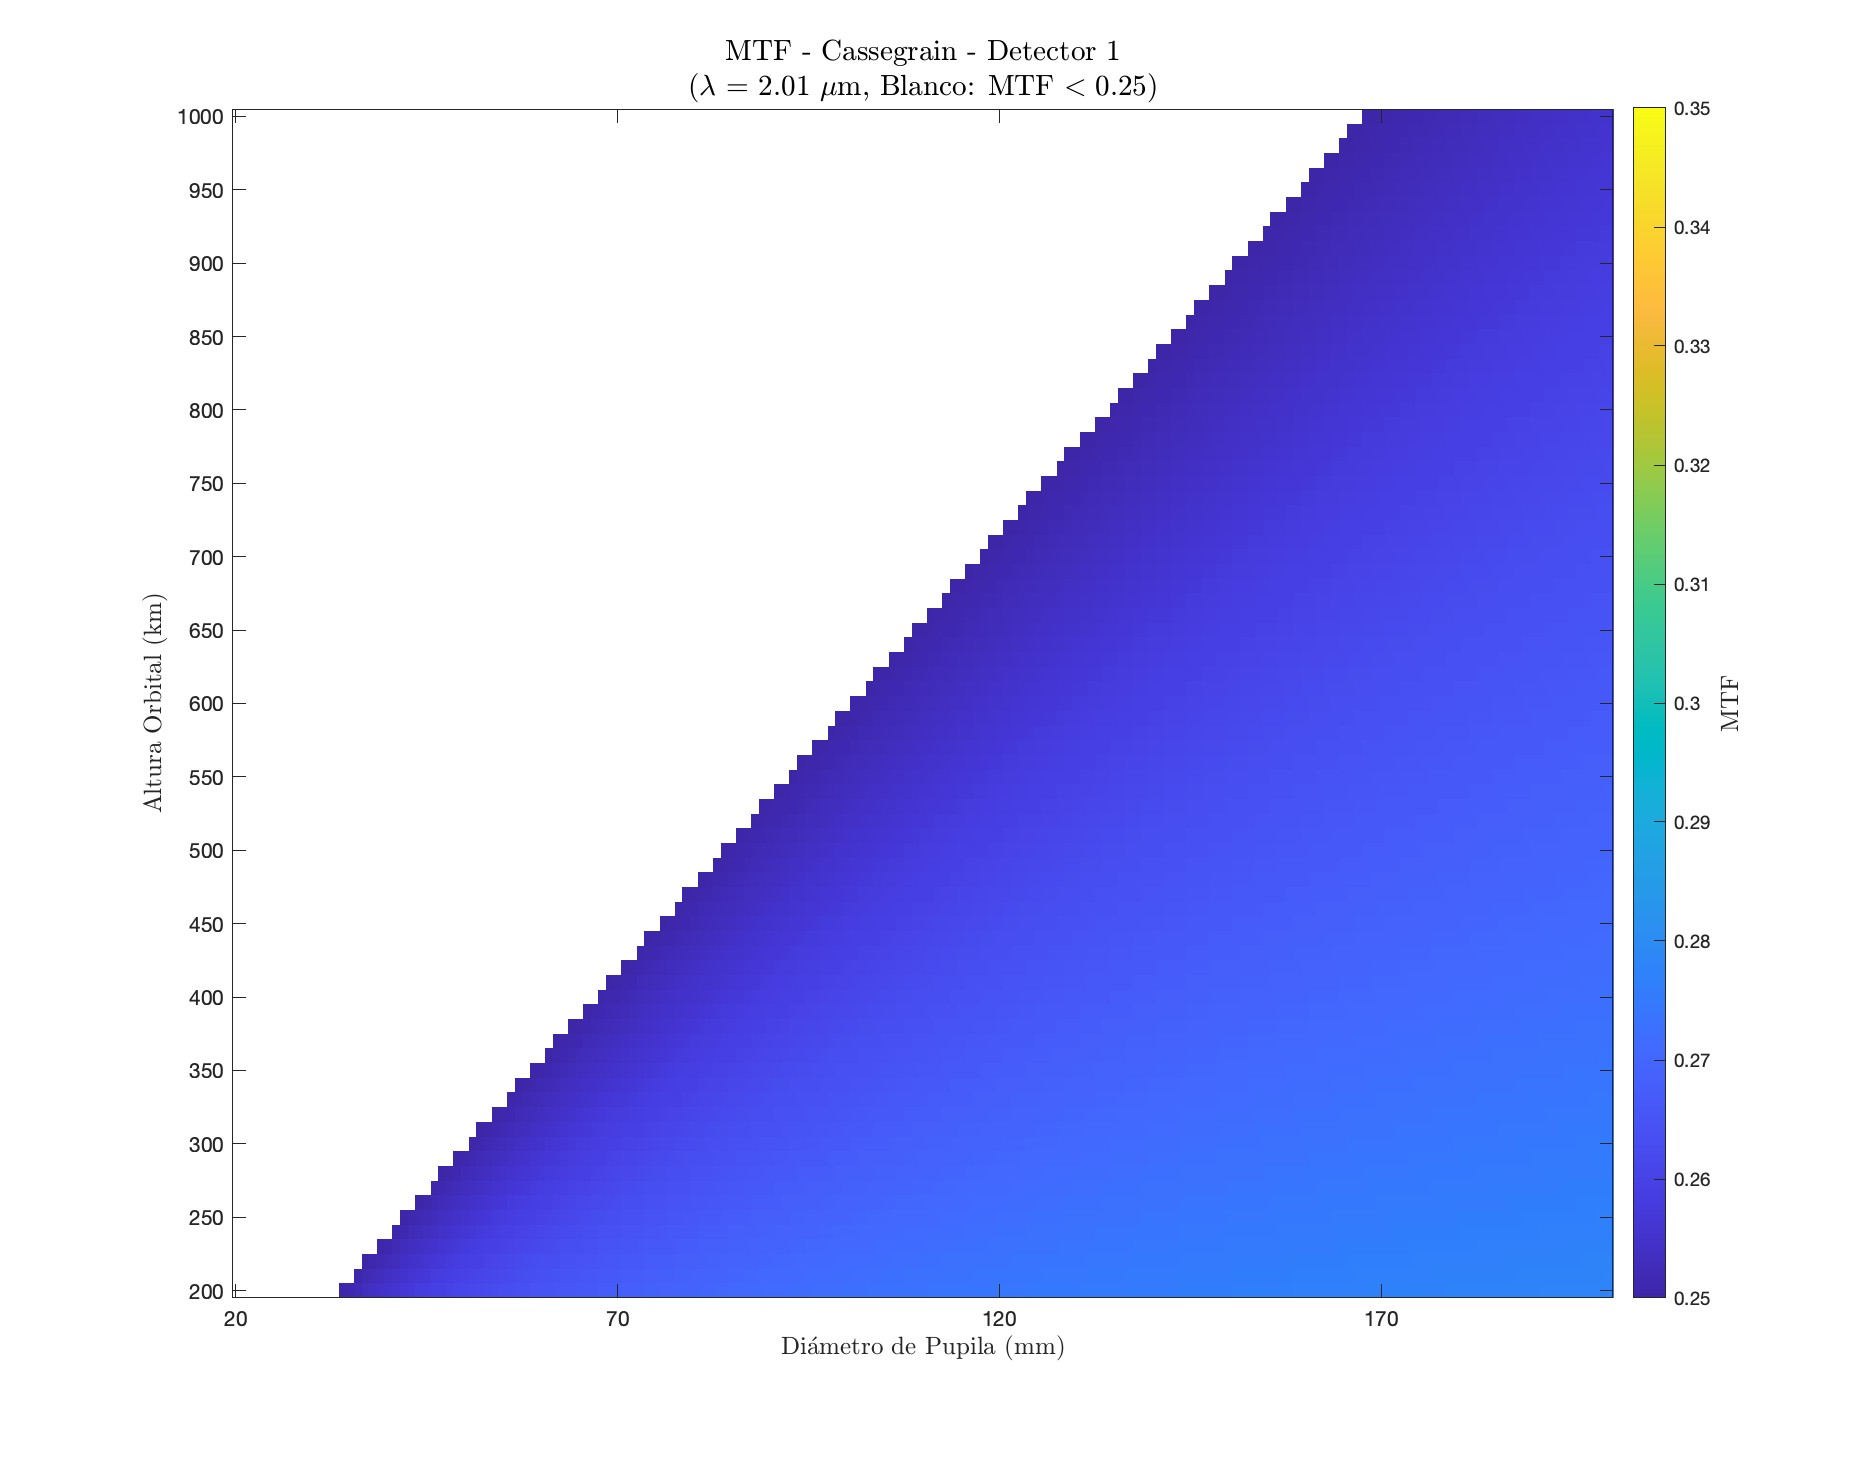
\includegraphics[width=0.48\linewidth]{4.Payload/MTF/MTF_Lambda2_Detector1_Telescopio3_heatmap.jpg} &
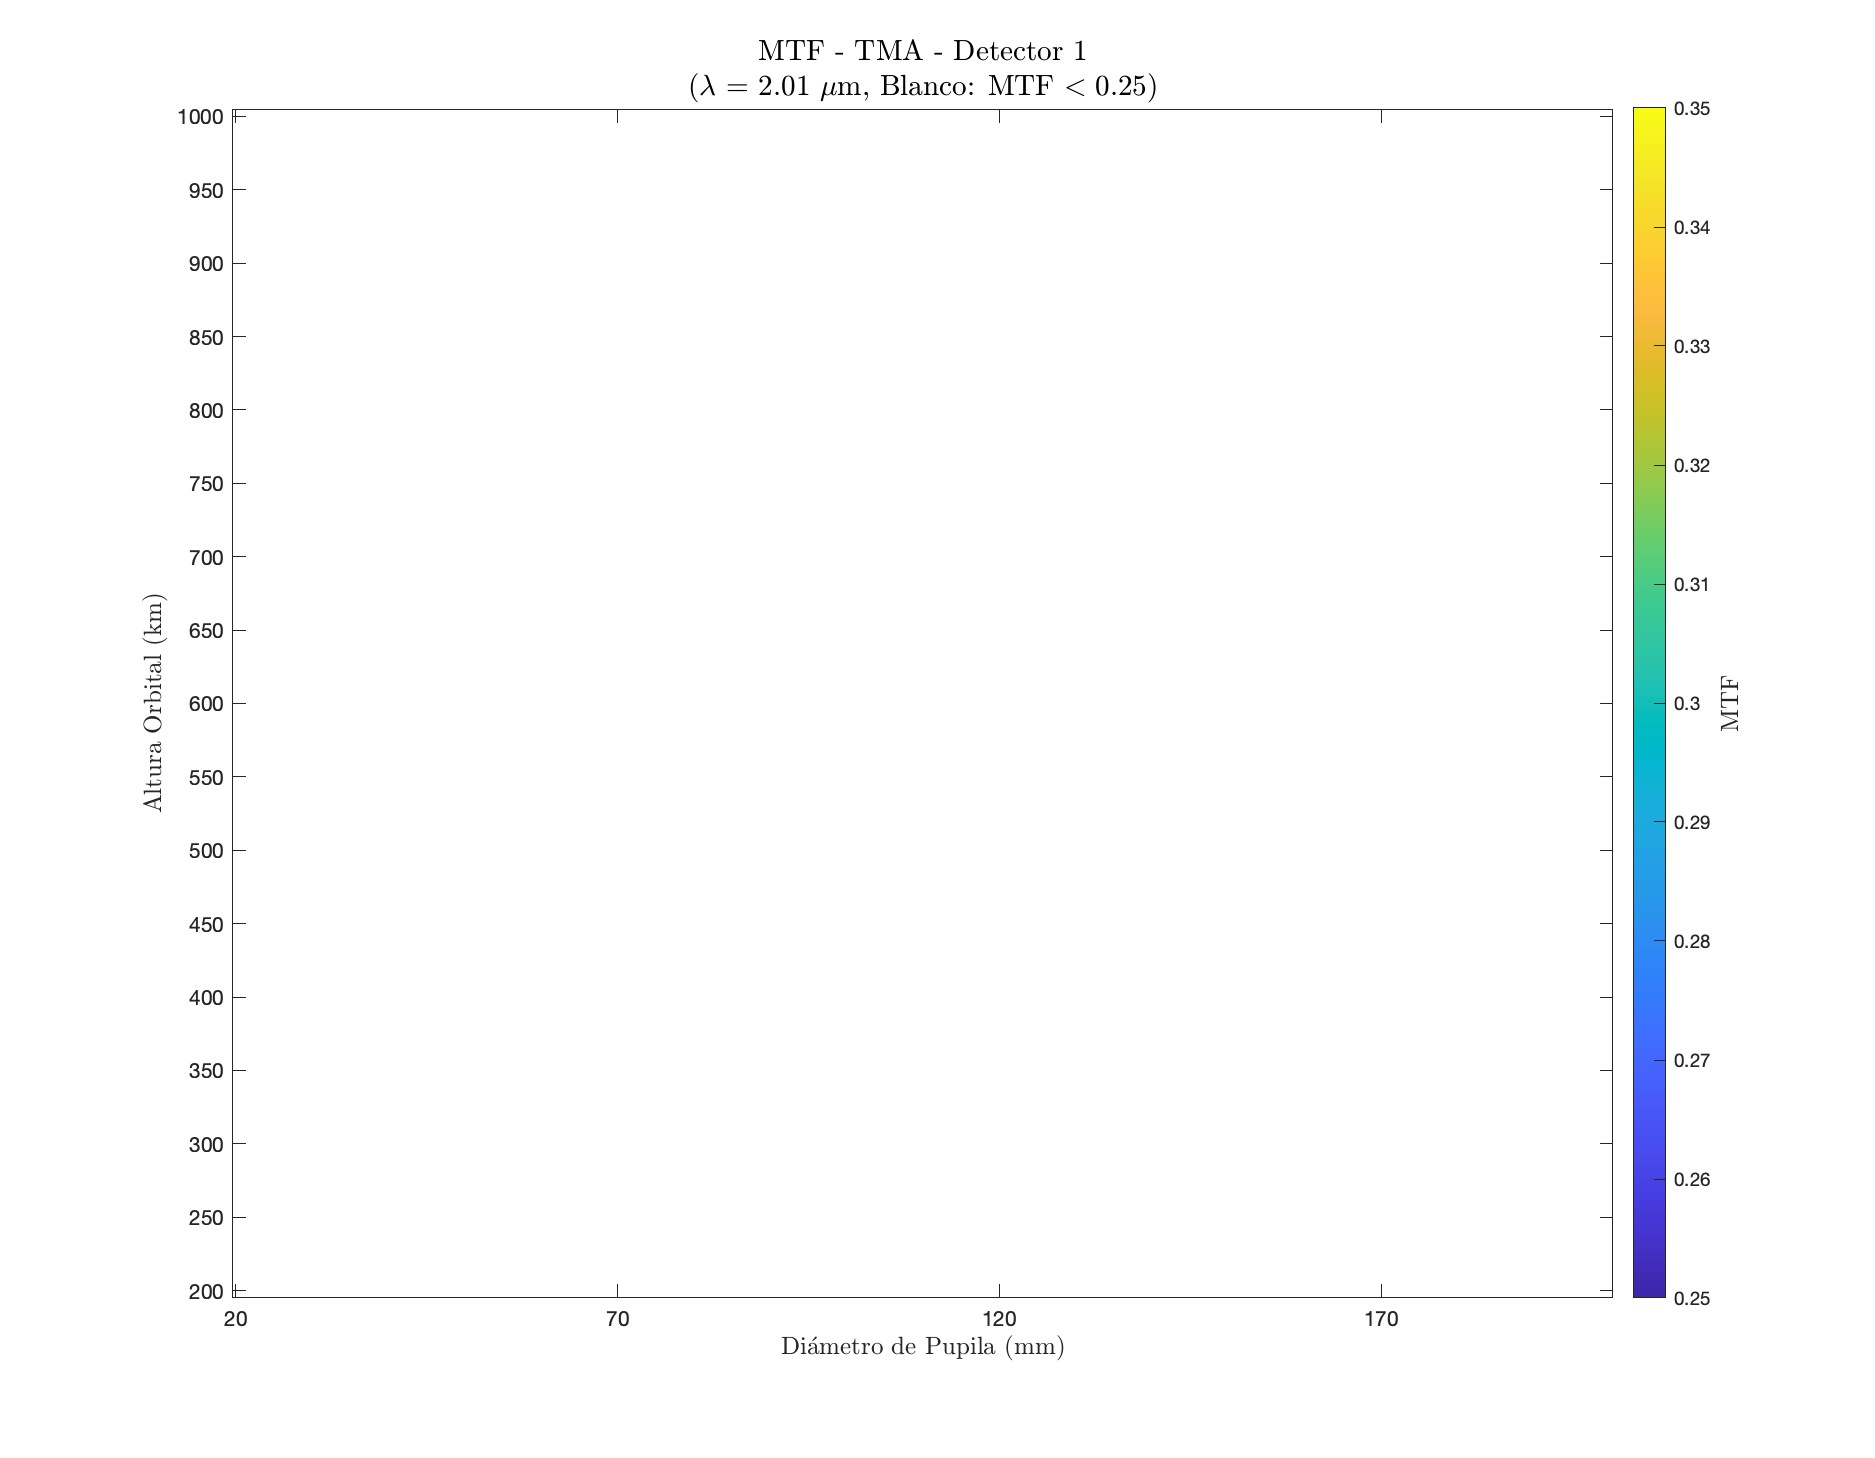
\includegraphics[width=0.48\linewidth]{4.Payload/MTF/MTF_Lambda2_Detector1_Telescopio4_heatmap.jpg} \\
\end{tabular}
\caption{Mapas de calor resultantes del calculo de MTF: Banda 2,01 \textmu m; Detector 1}
\end{figure}
\end{landscape}


%% DETECTOR 2
\begin{landscape}
\begin{figure}[p]
\centering
\setlength{\tabcolsep}{2pt}
\renewcommand{\arraystretch}{0}

\begin{tabular}{cc}
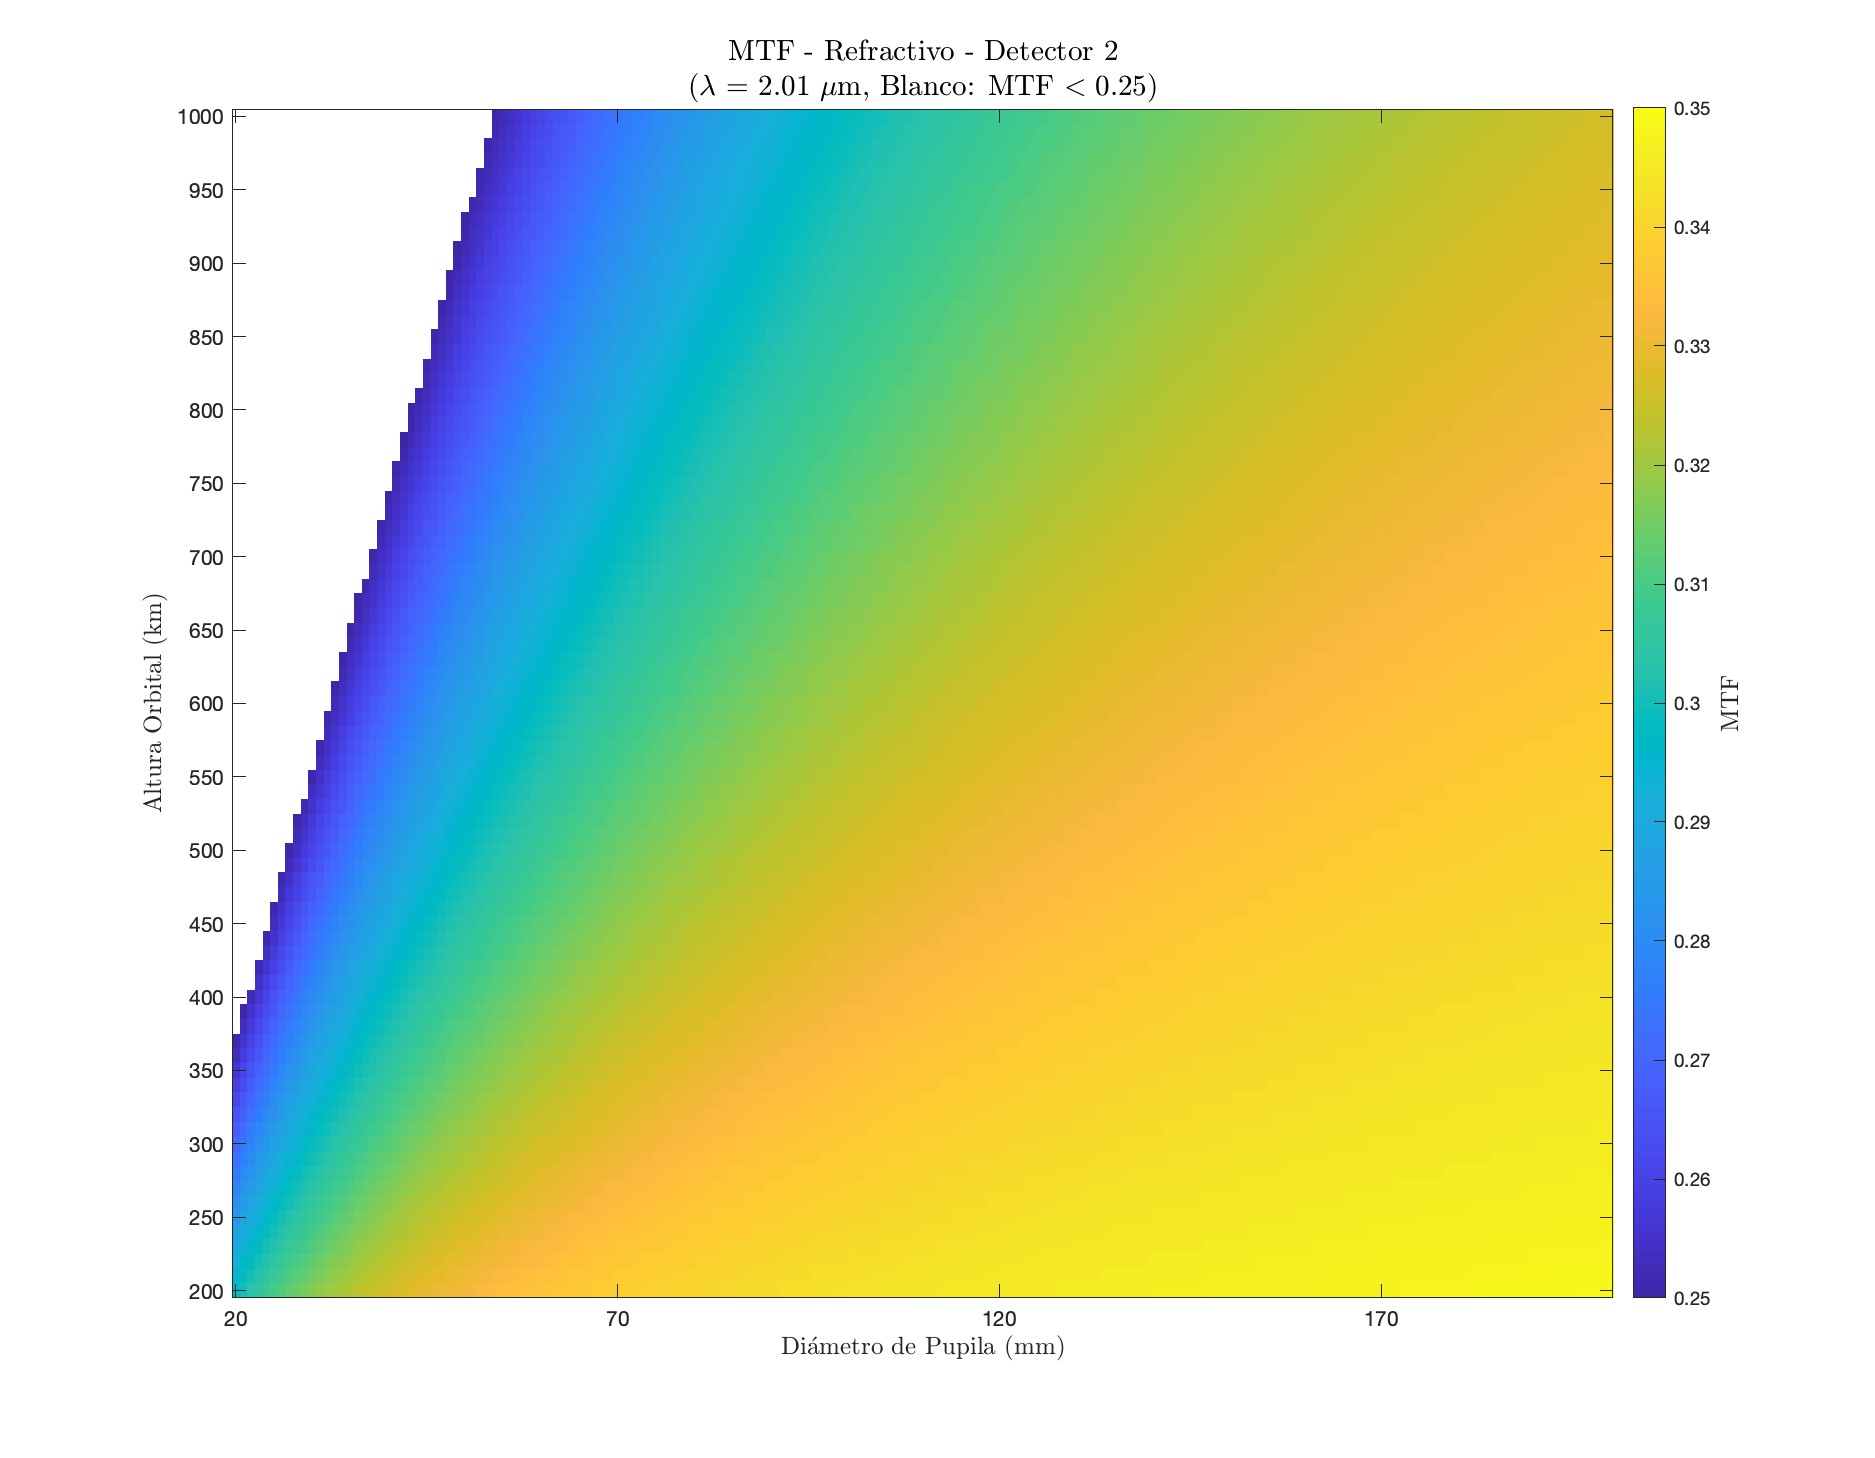
\includegraphics[width=0.48\linewidth]{4.Payload/MTF/MTF_Lambda2_Detector2_Telescopio1_heatmap.jpg} &
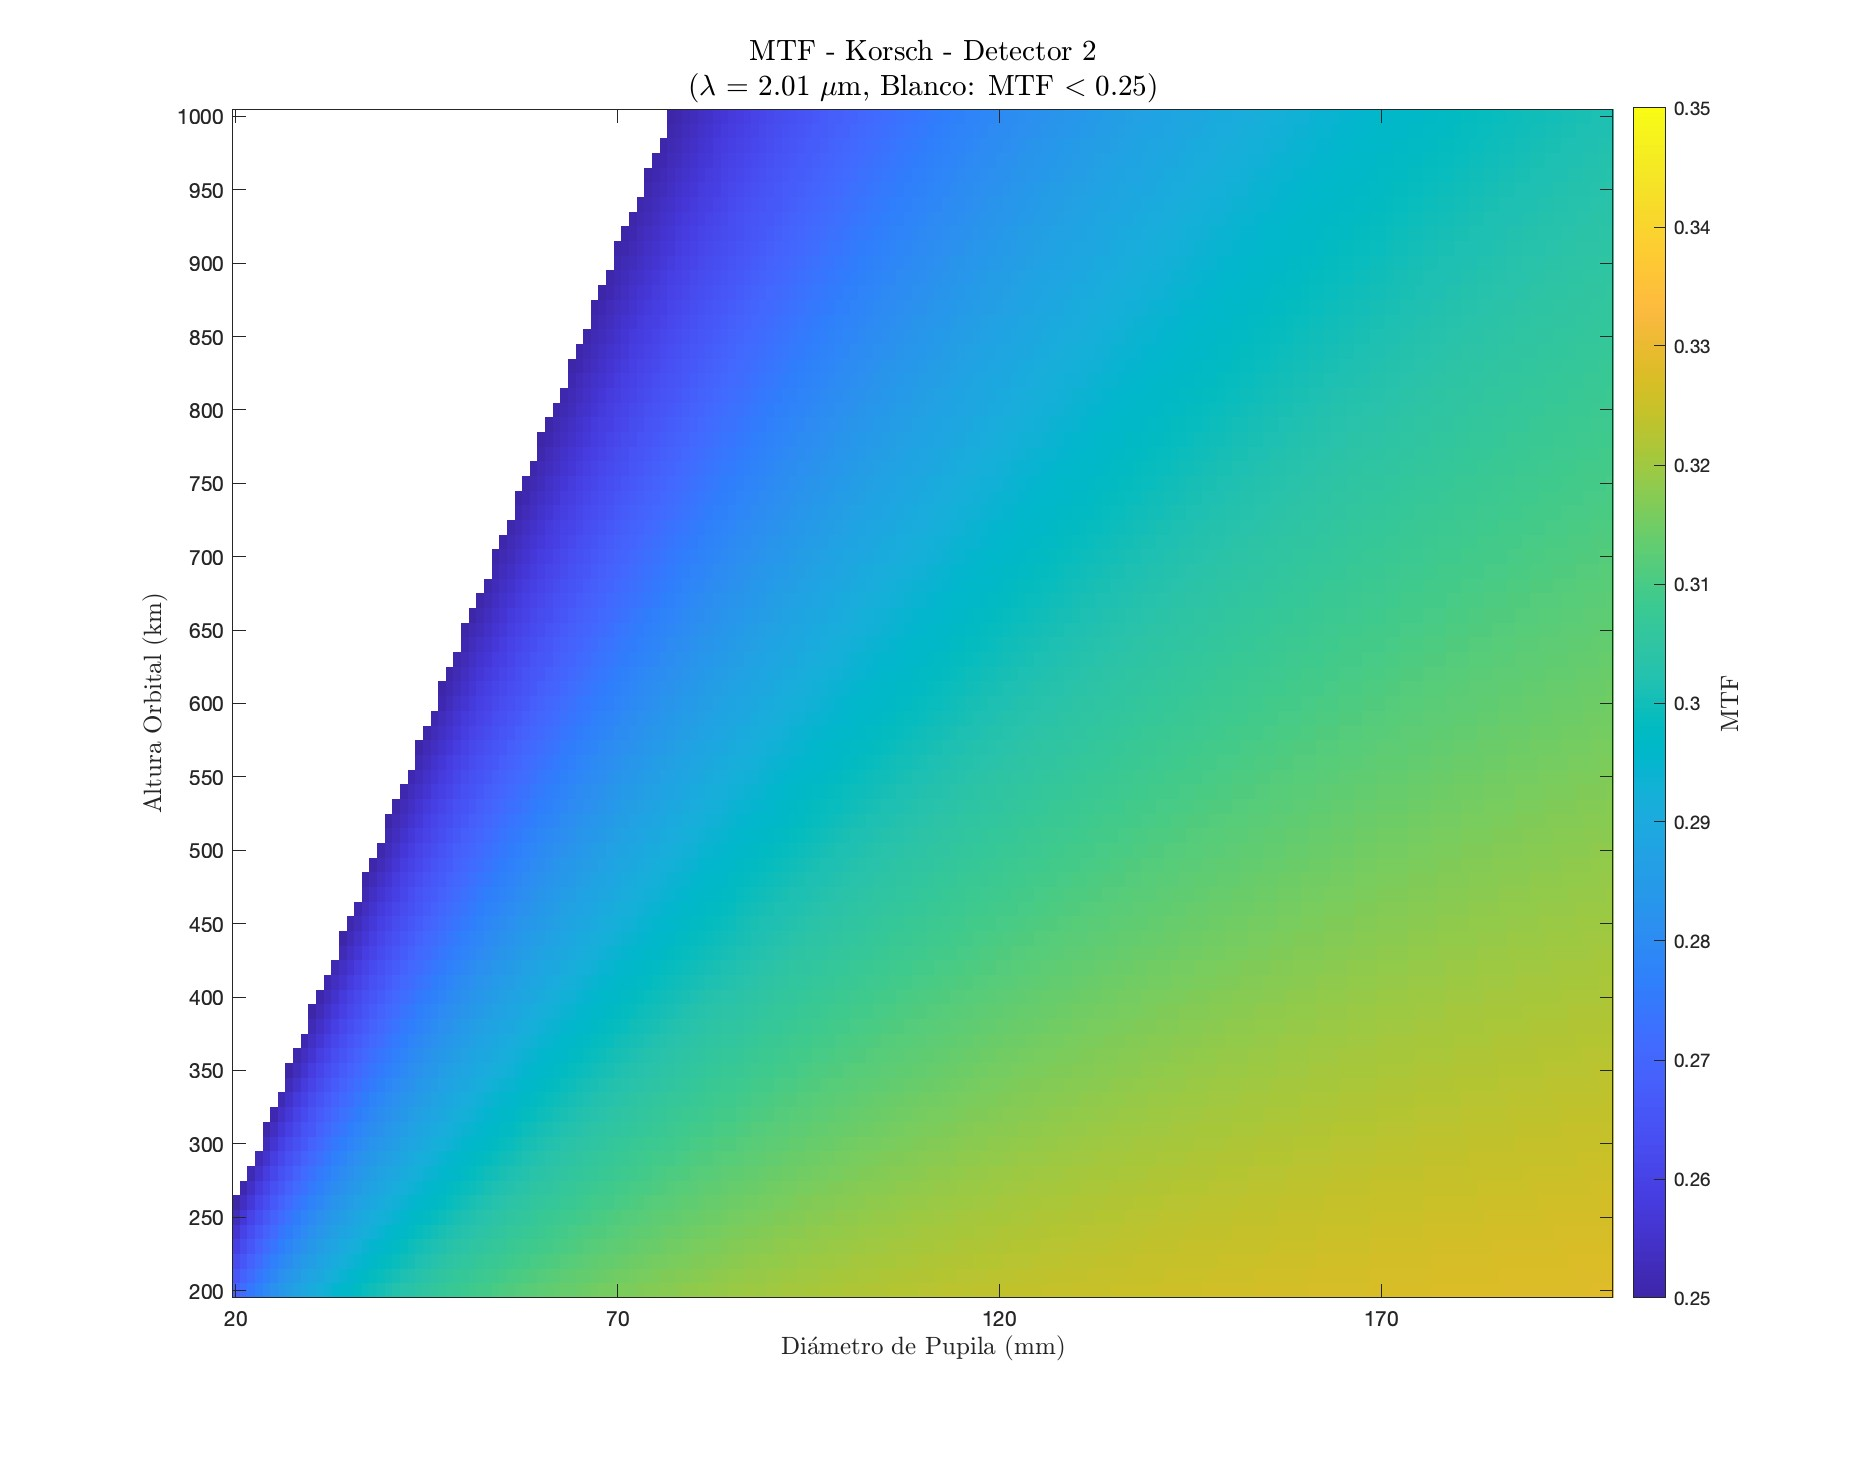
\includegraphics[width=0.48\linewidth]{4.Payload/MTF/MTF_Lambda2_Detector2_Telescopio2_heatmap.jpg} \\
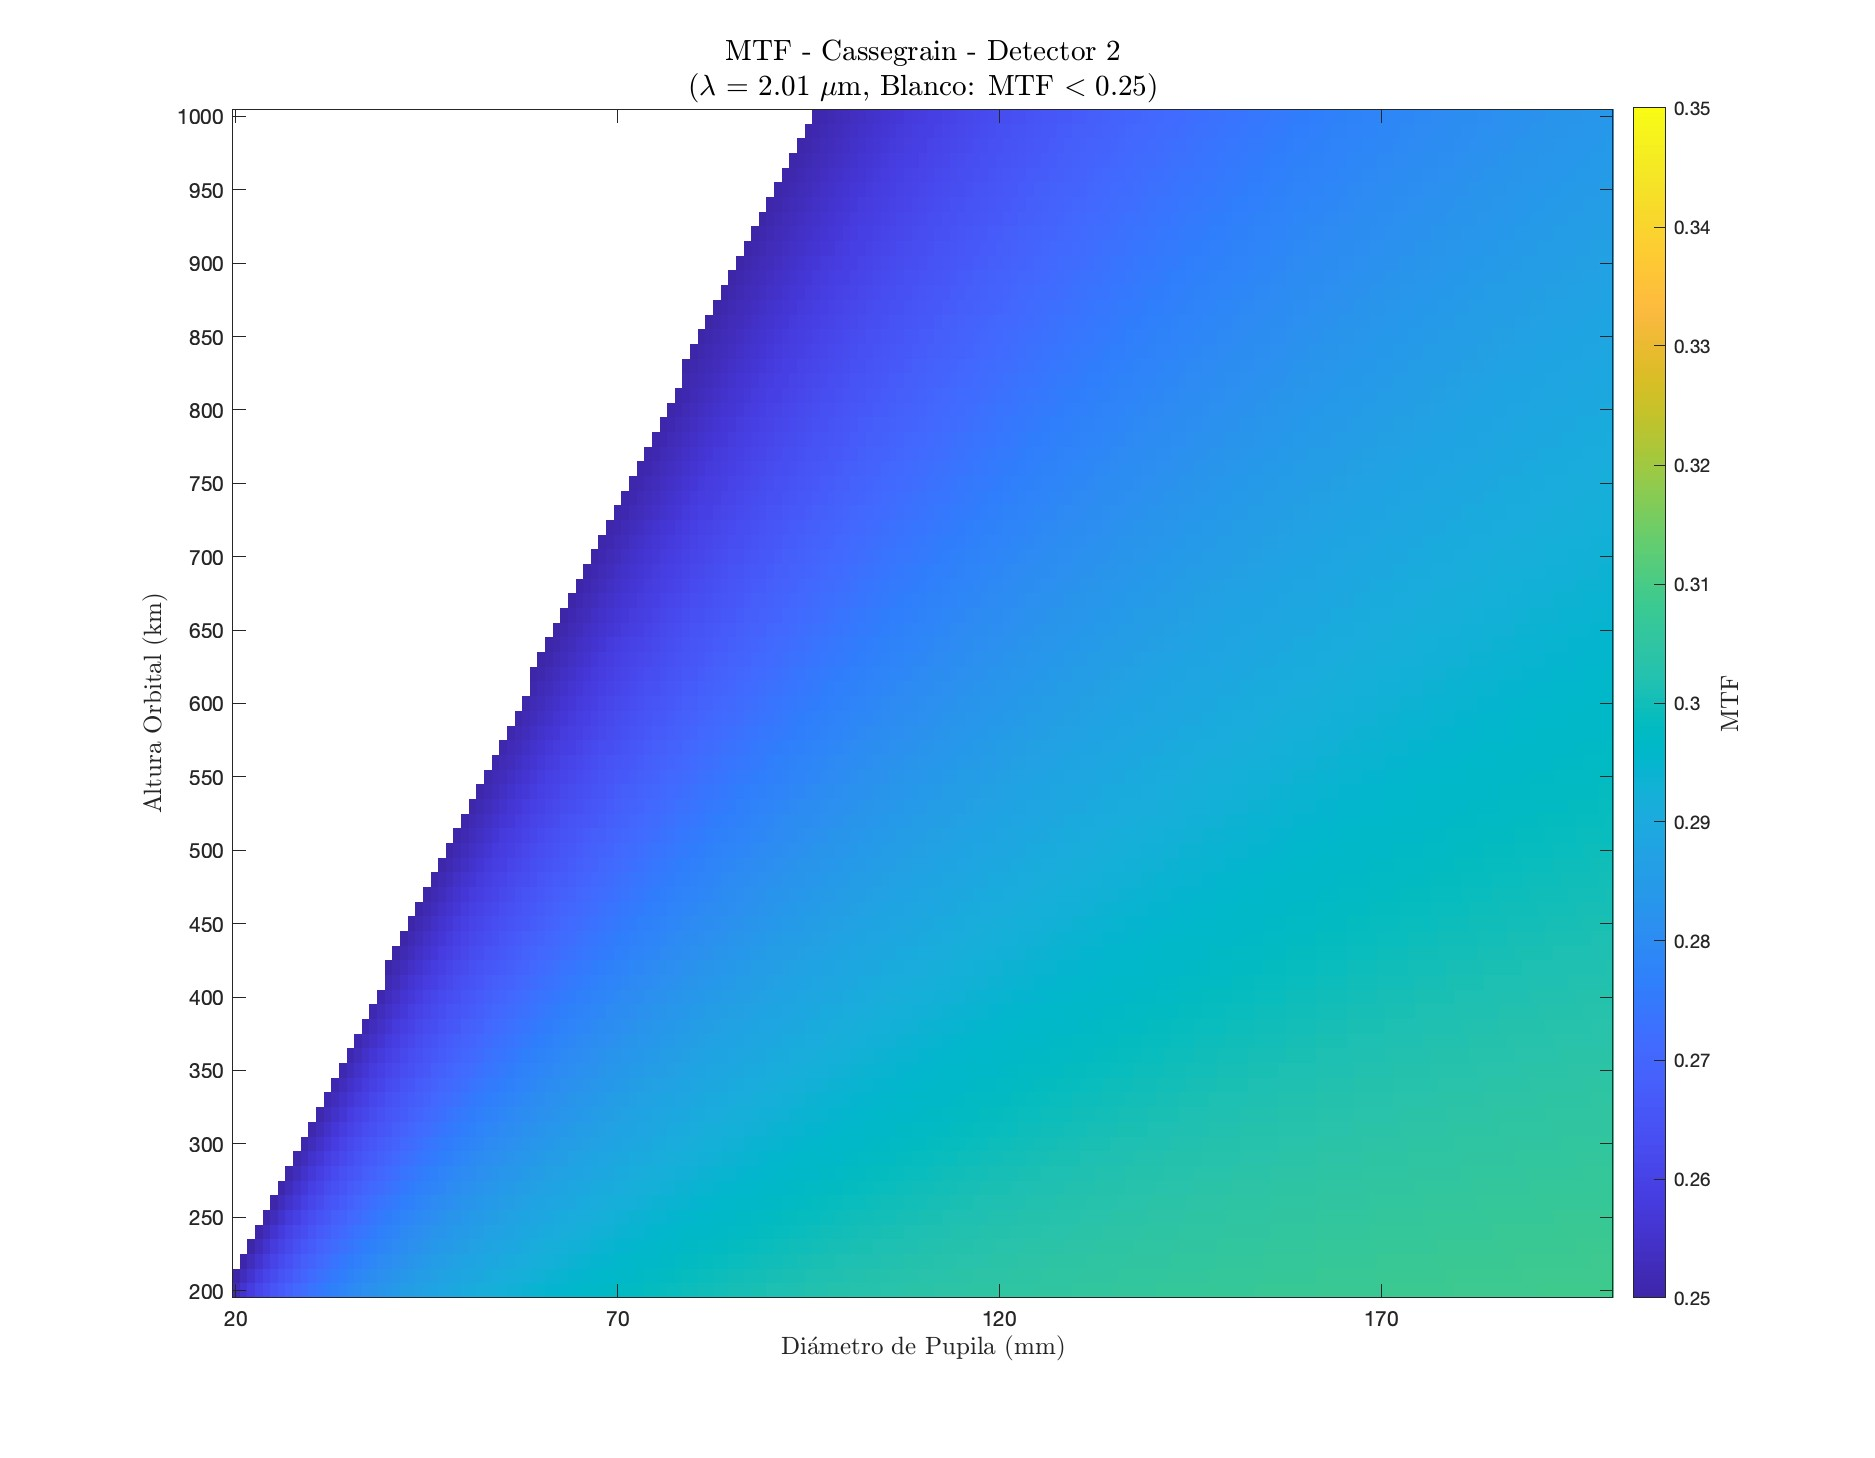
\includegraphics[width=0.48\linewidth]{4.Payload/MTF/MTF_Lambda2_Detector2_Telescopio3_heatmap.jpg} &
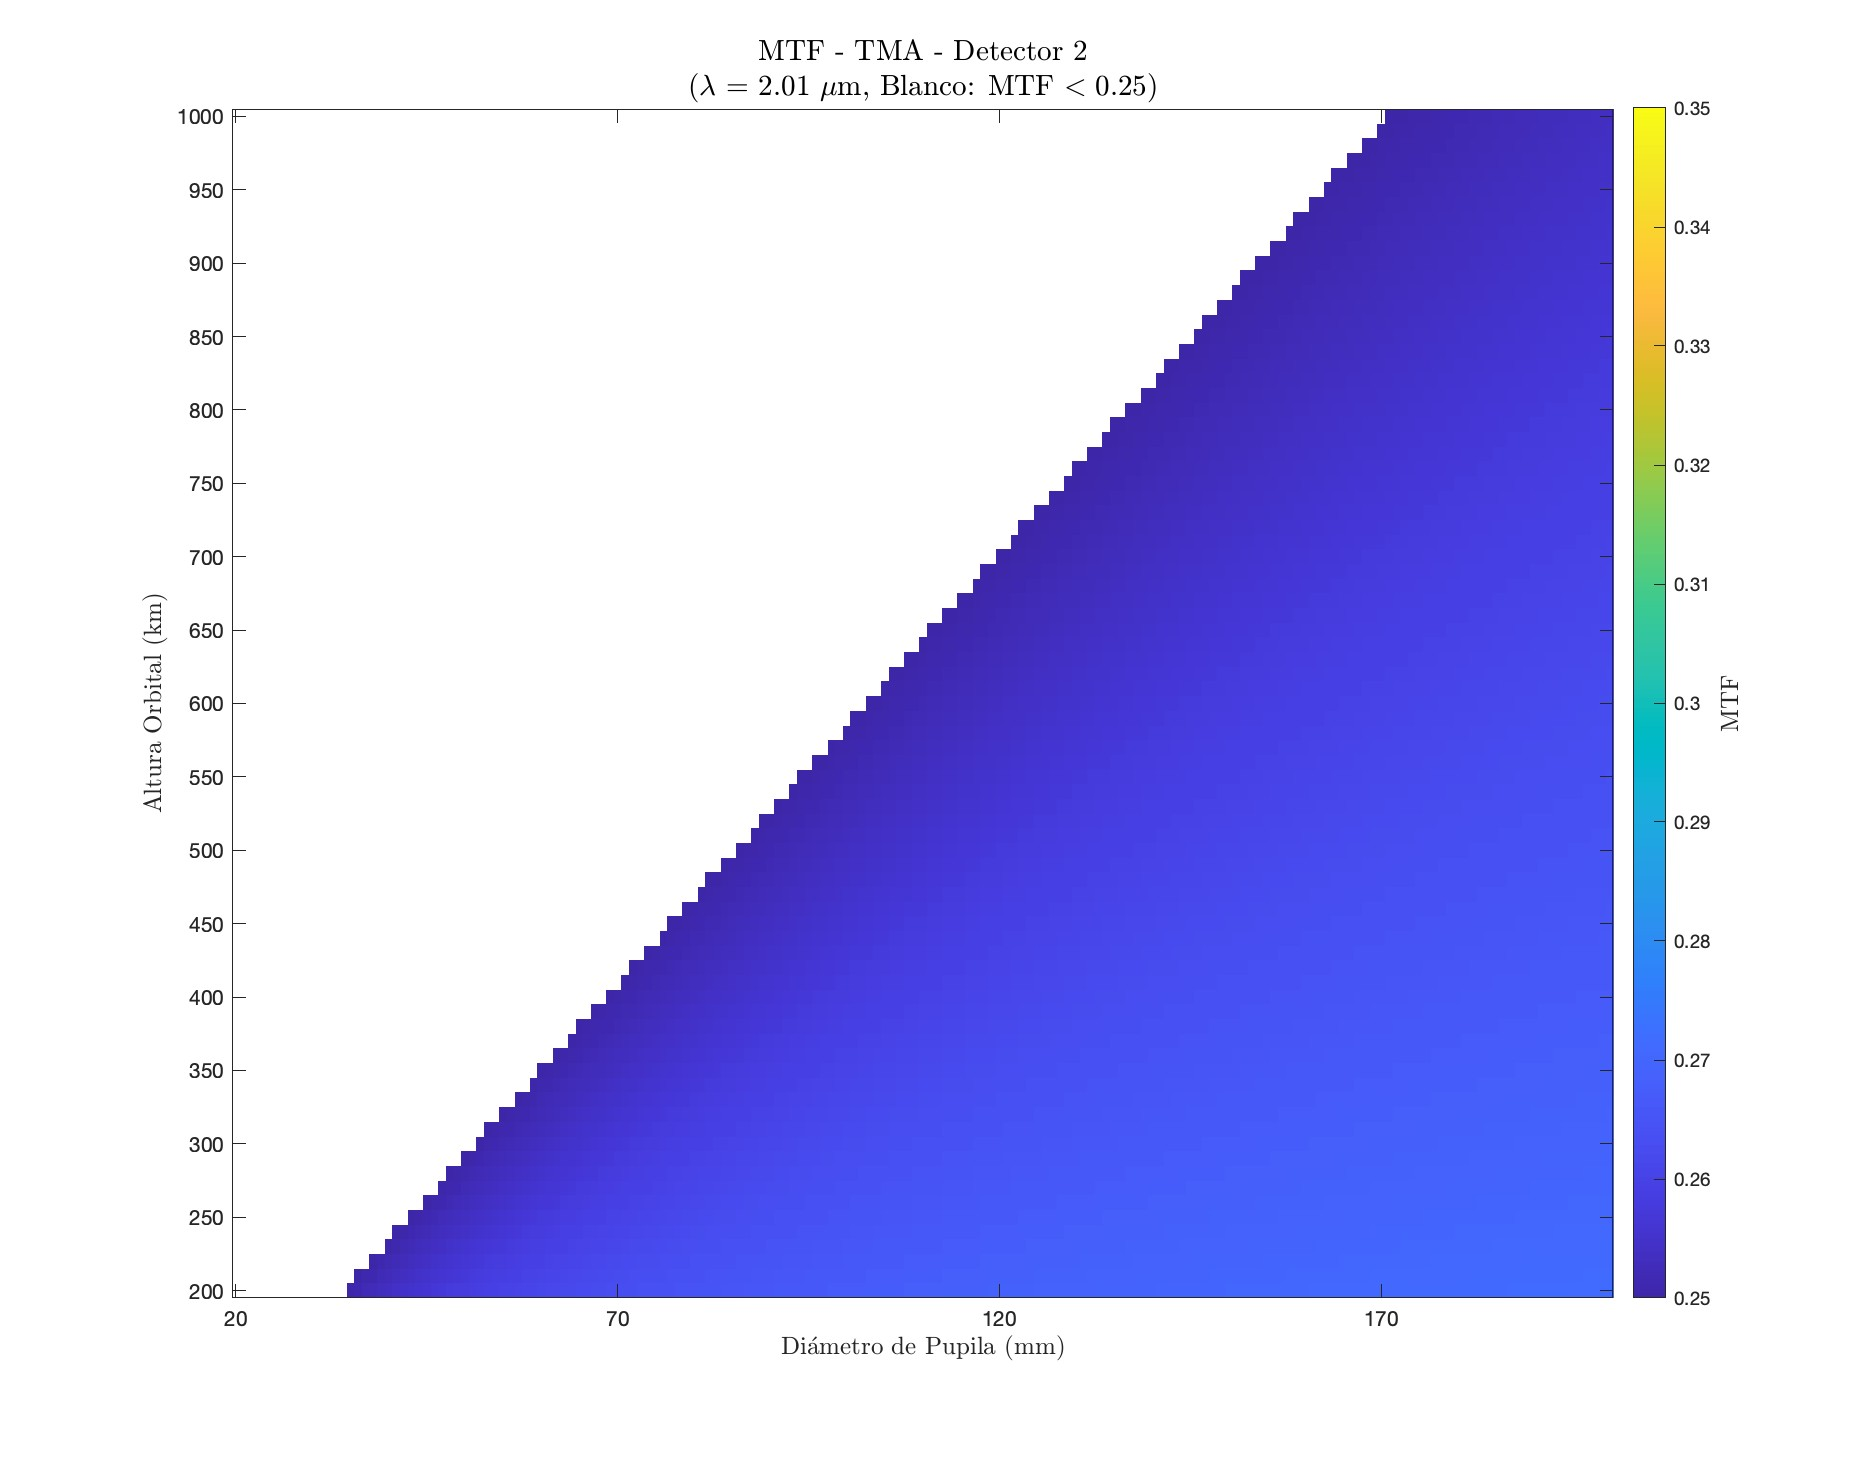
\includegraphics[width=0.48\linewidth]{4.Payload/MTF/MTF_Lambda2_Detector2_Telescopio4_heatmap.jpg} \\
\end{tabular}
\caption{Mapas de calor resultantes del calculo de MTF: Banda 2,01 \textmu m; Detector 2}
\end{figure}
\end{landscape}


%% DETECTOR 3
\begin{landscape}
\begin{figure}[p]
\centering
\setlength{\tabcolsep}{2pt}
\renewcommand{\arraystretch}{0}

\begin{tabular}{cc}
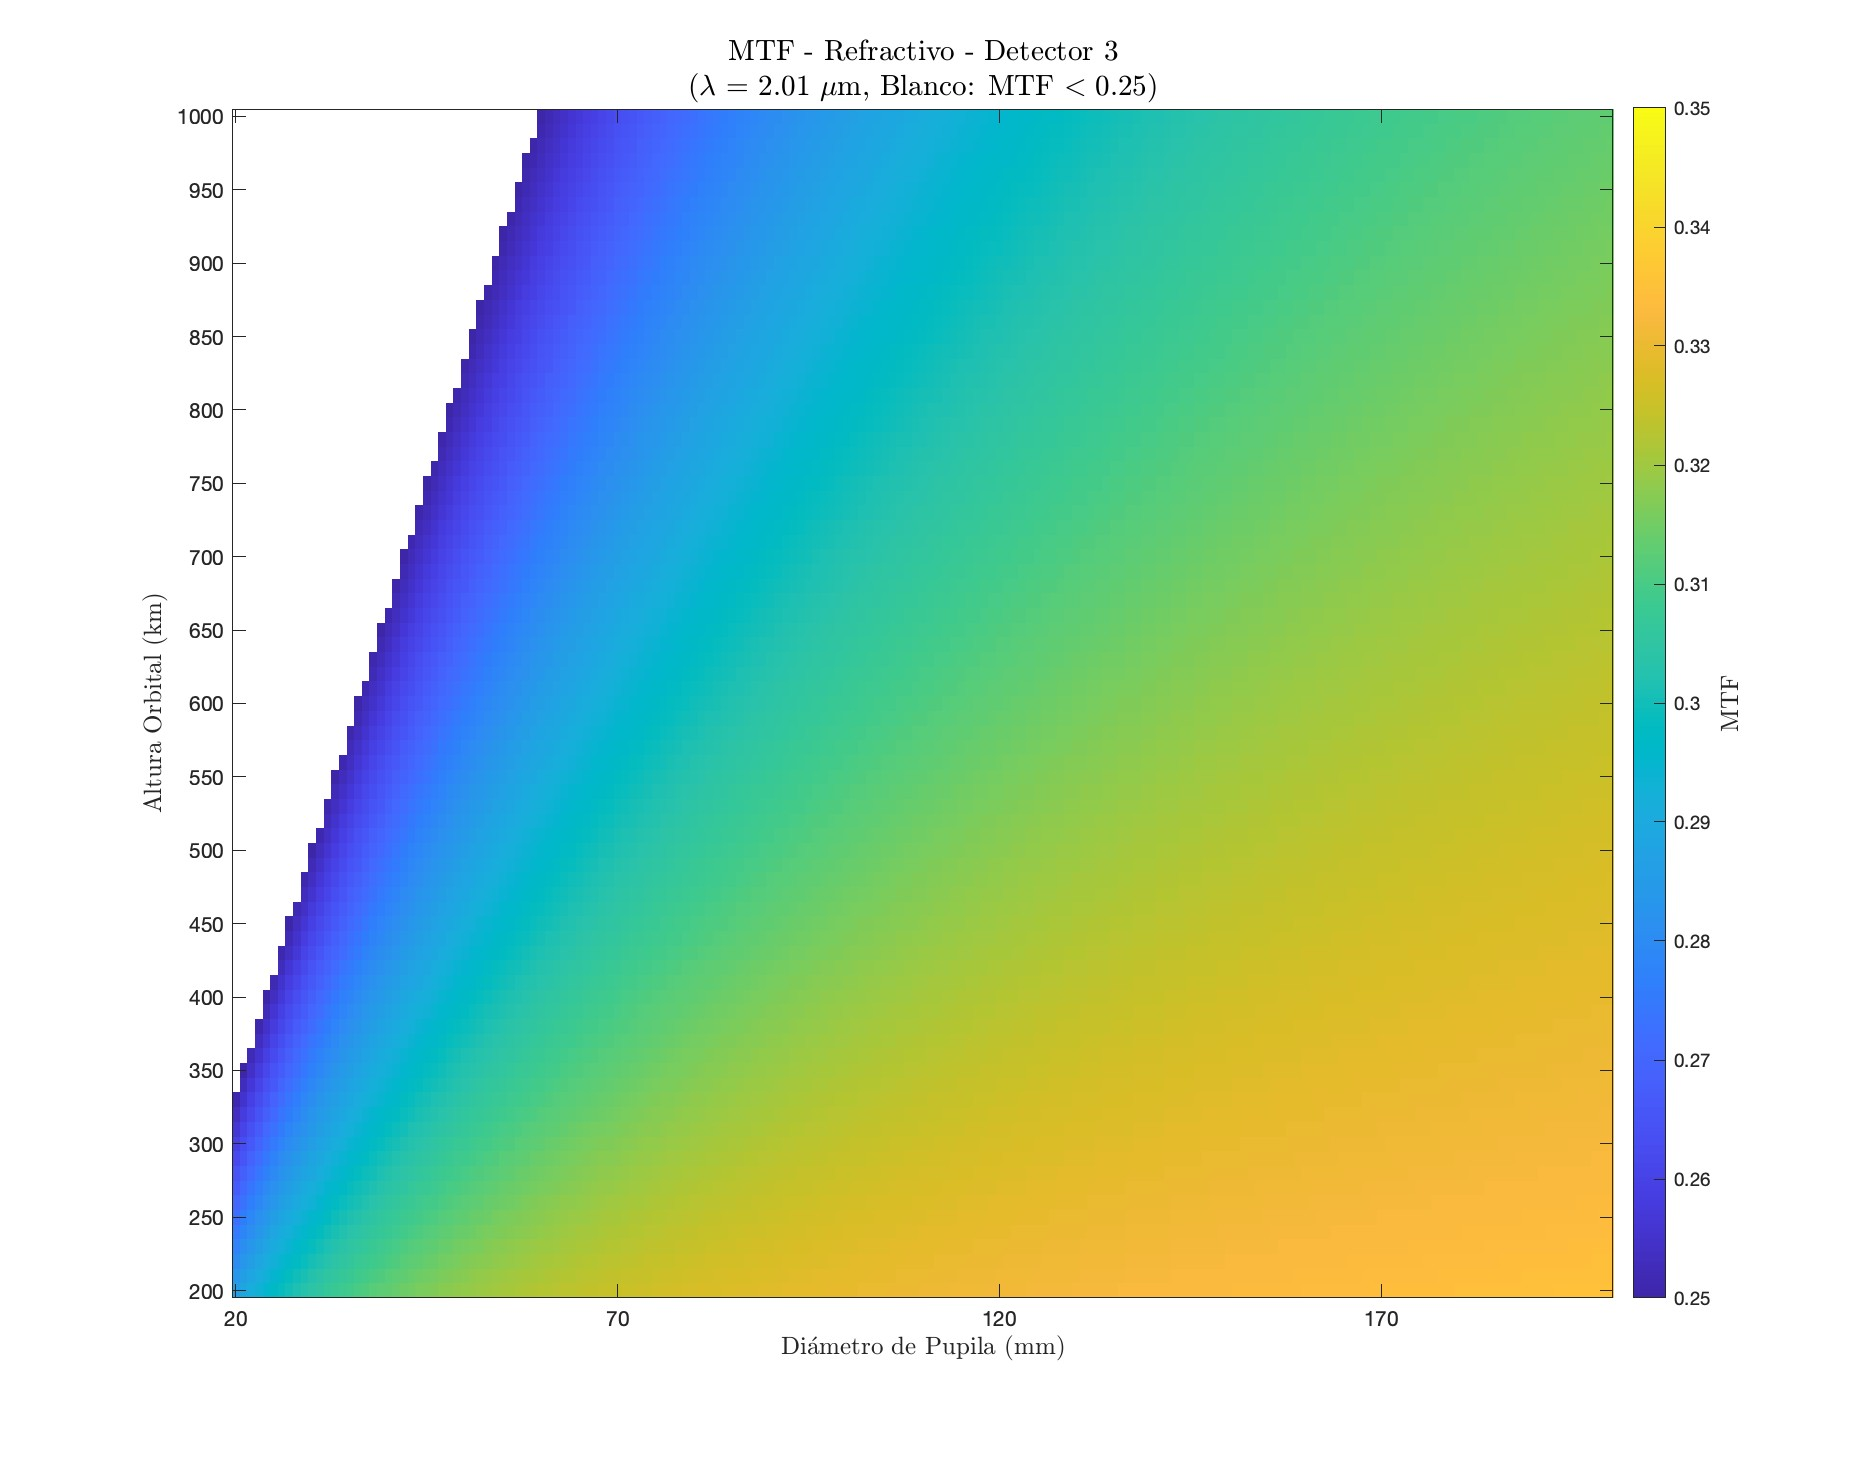
\includegraphics[width=0.48\linewidth]{4.Payload/MTF/MTF_Lambda2_Detector3_Telescopio1_heatmap.jpg} &
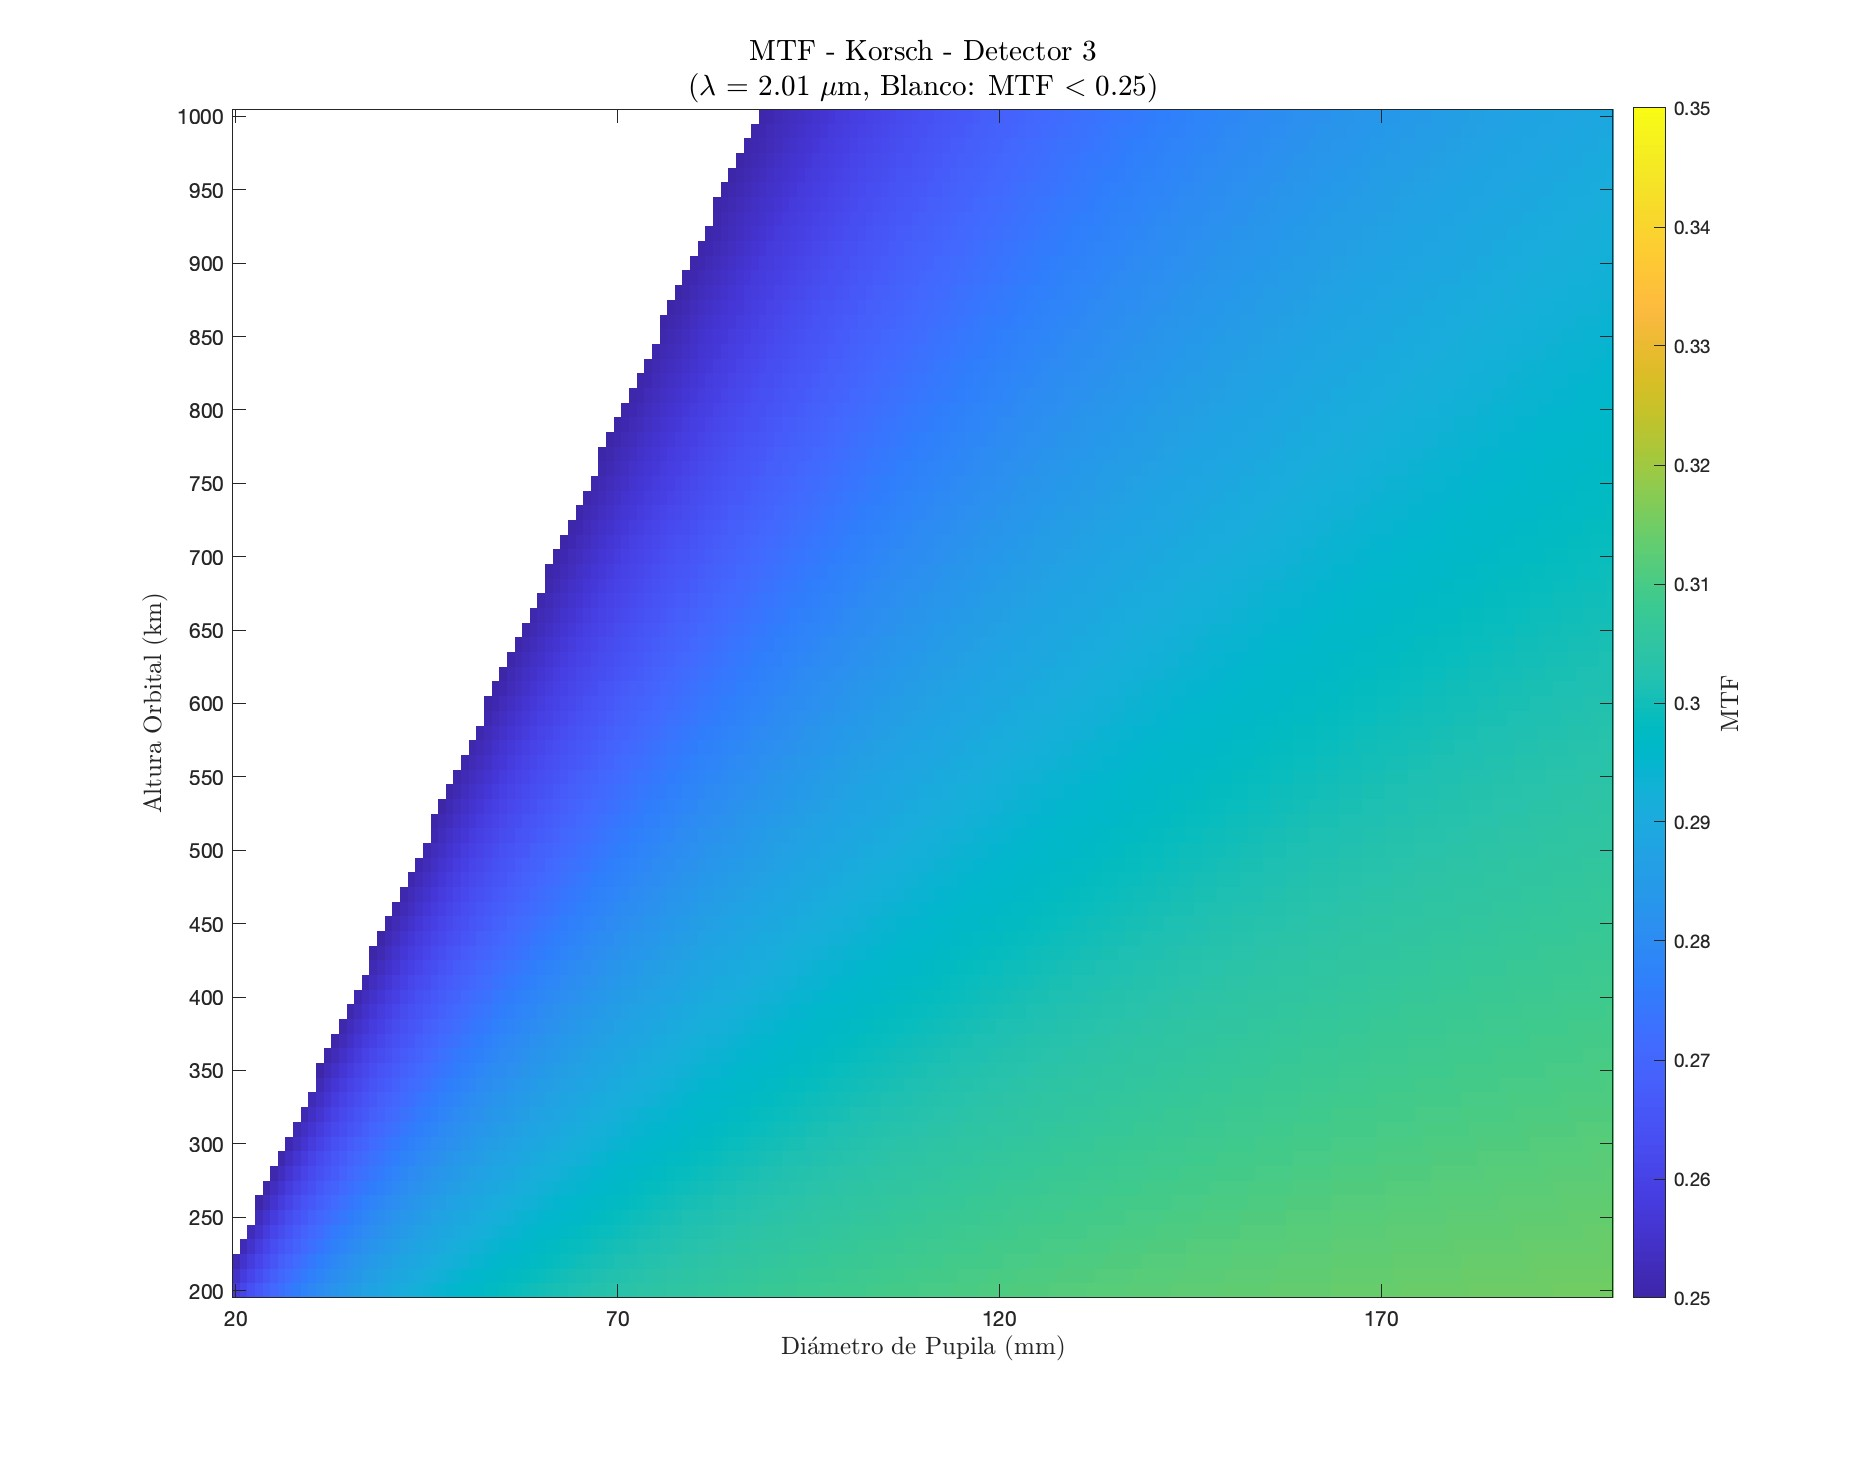
\includegraphics[width=0.48\linewidth]{4.Payload/MTF/MTF_Lambda2_Detector3_Telescopio2_heatmap.jpg} \\
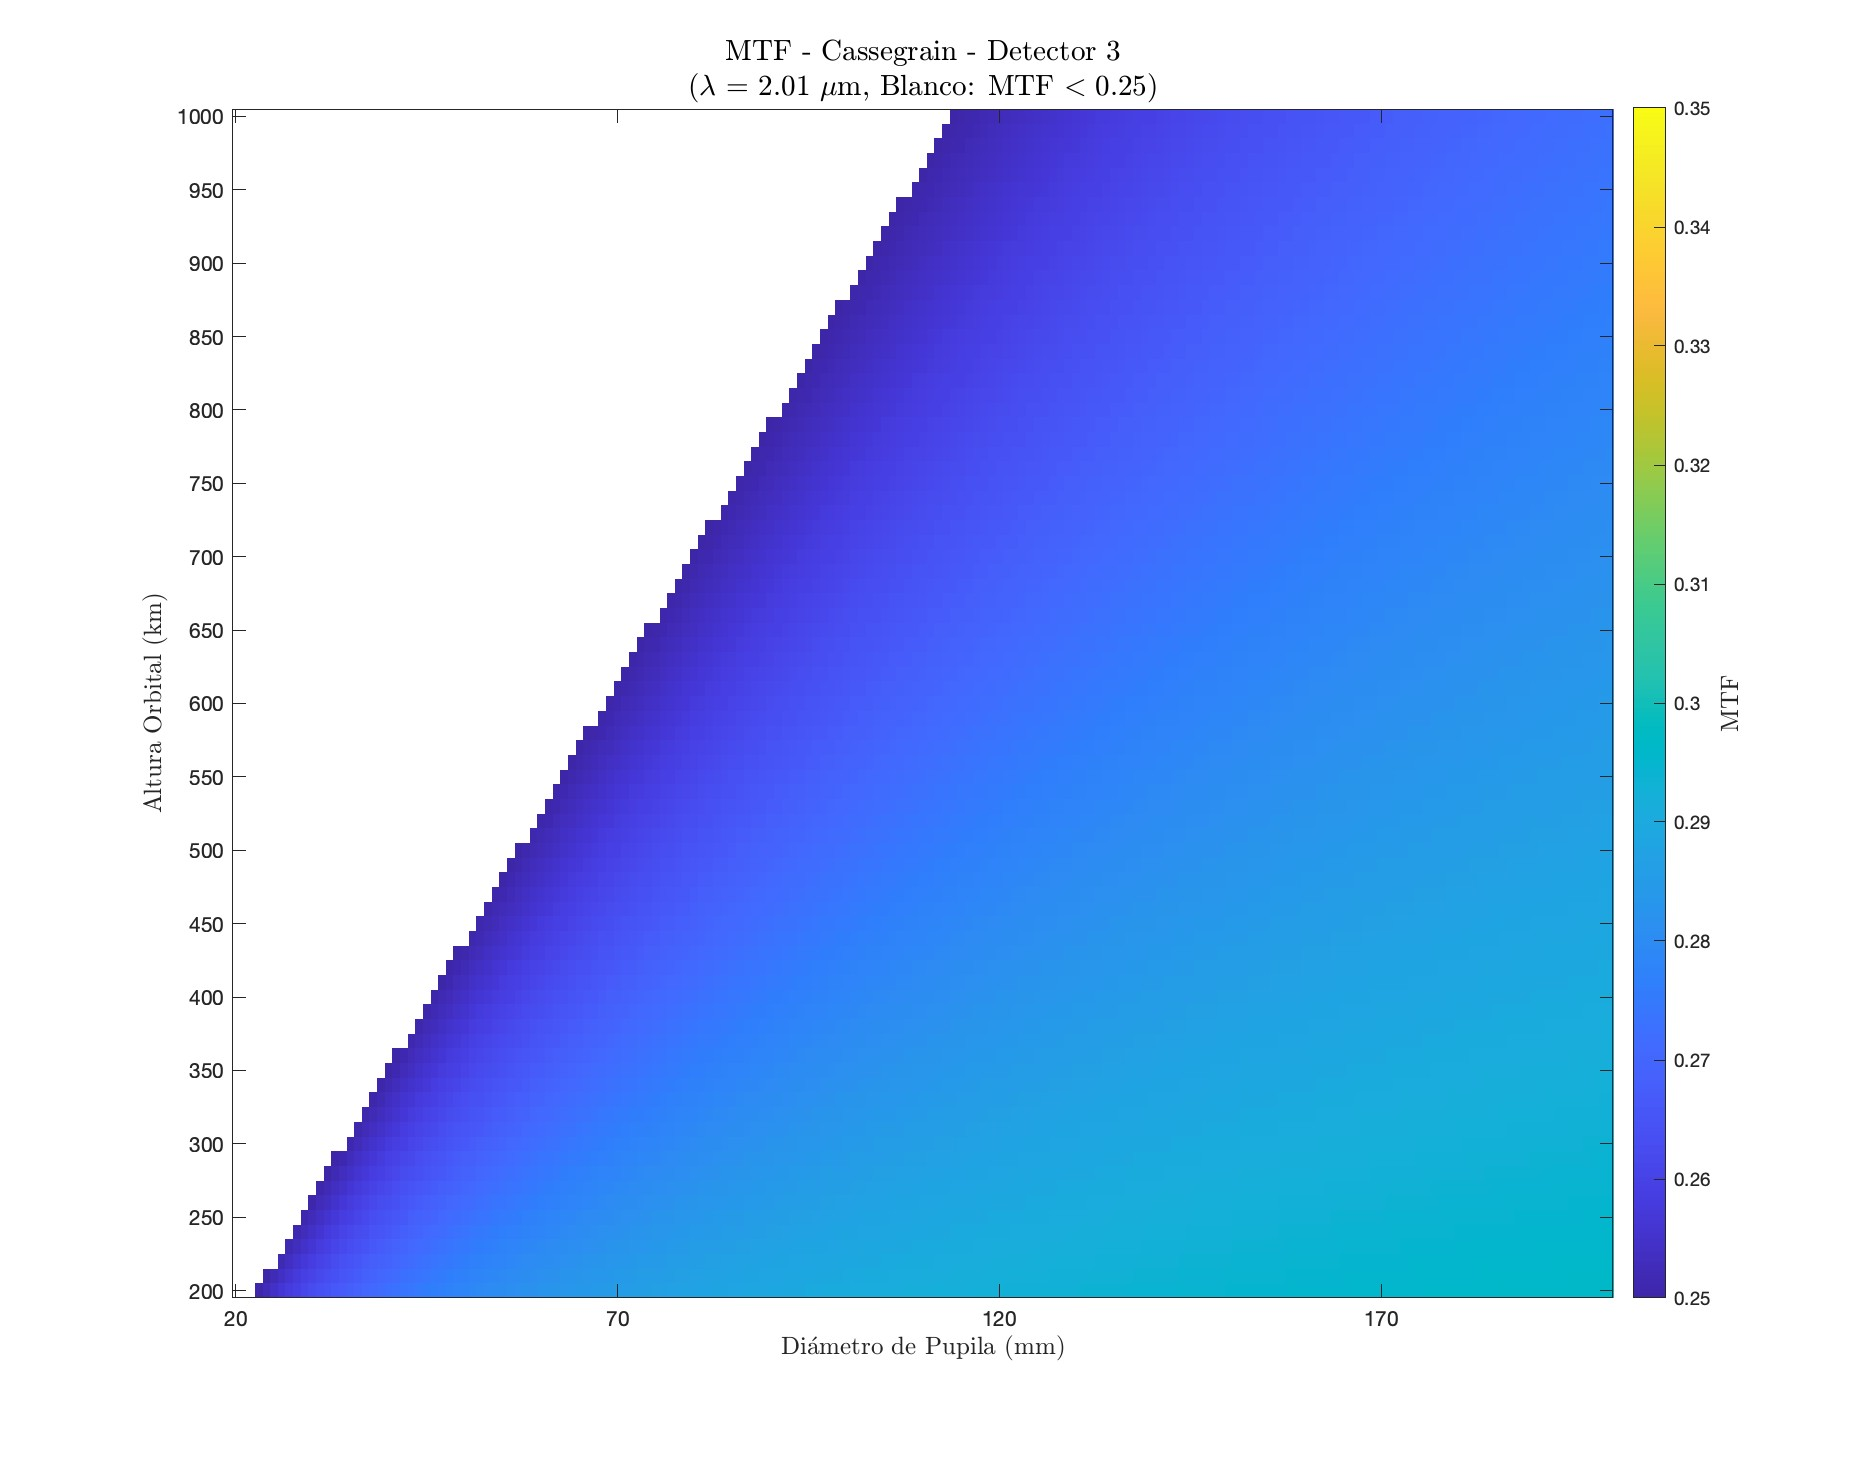
\includegraphics[width=0.48\linewidth]{4.Payload/MTF/MTF_Lambda2_Detector3_Telescopio3_heatmap.jpg} &
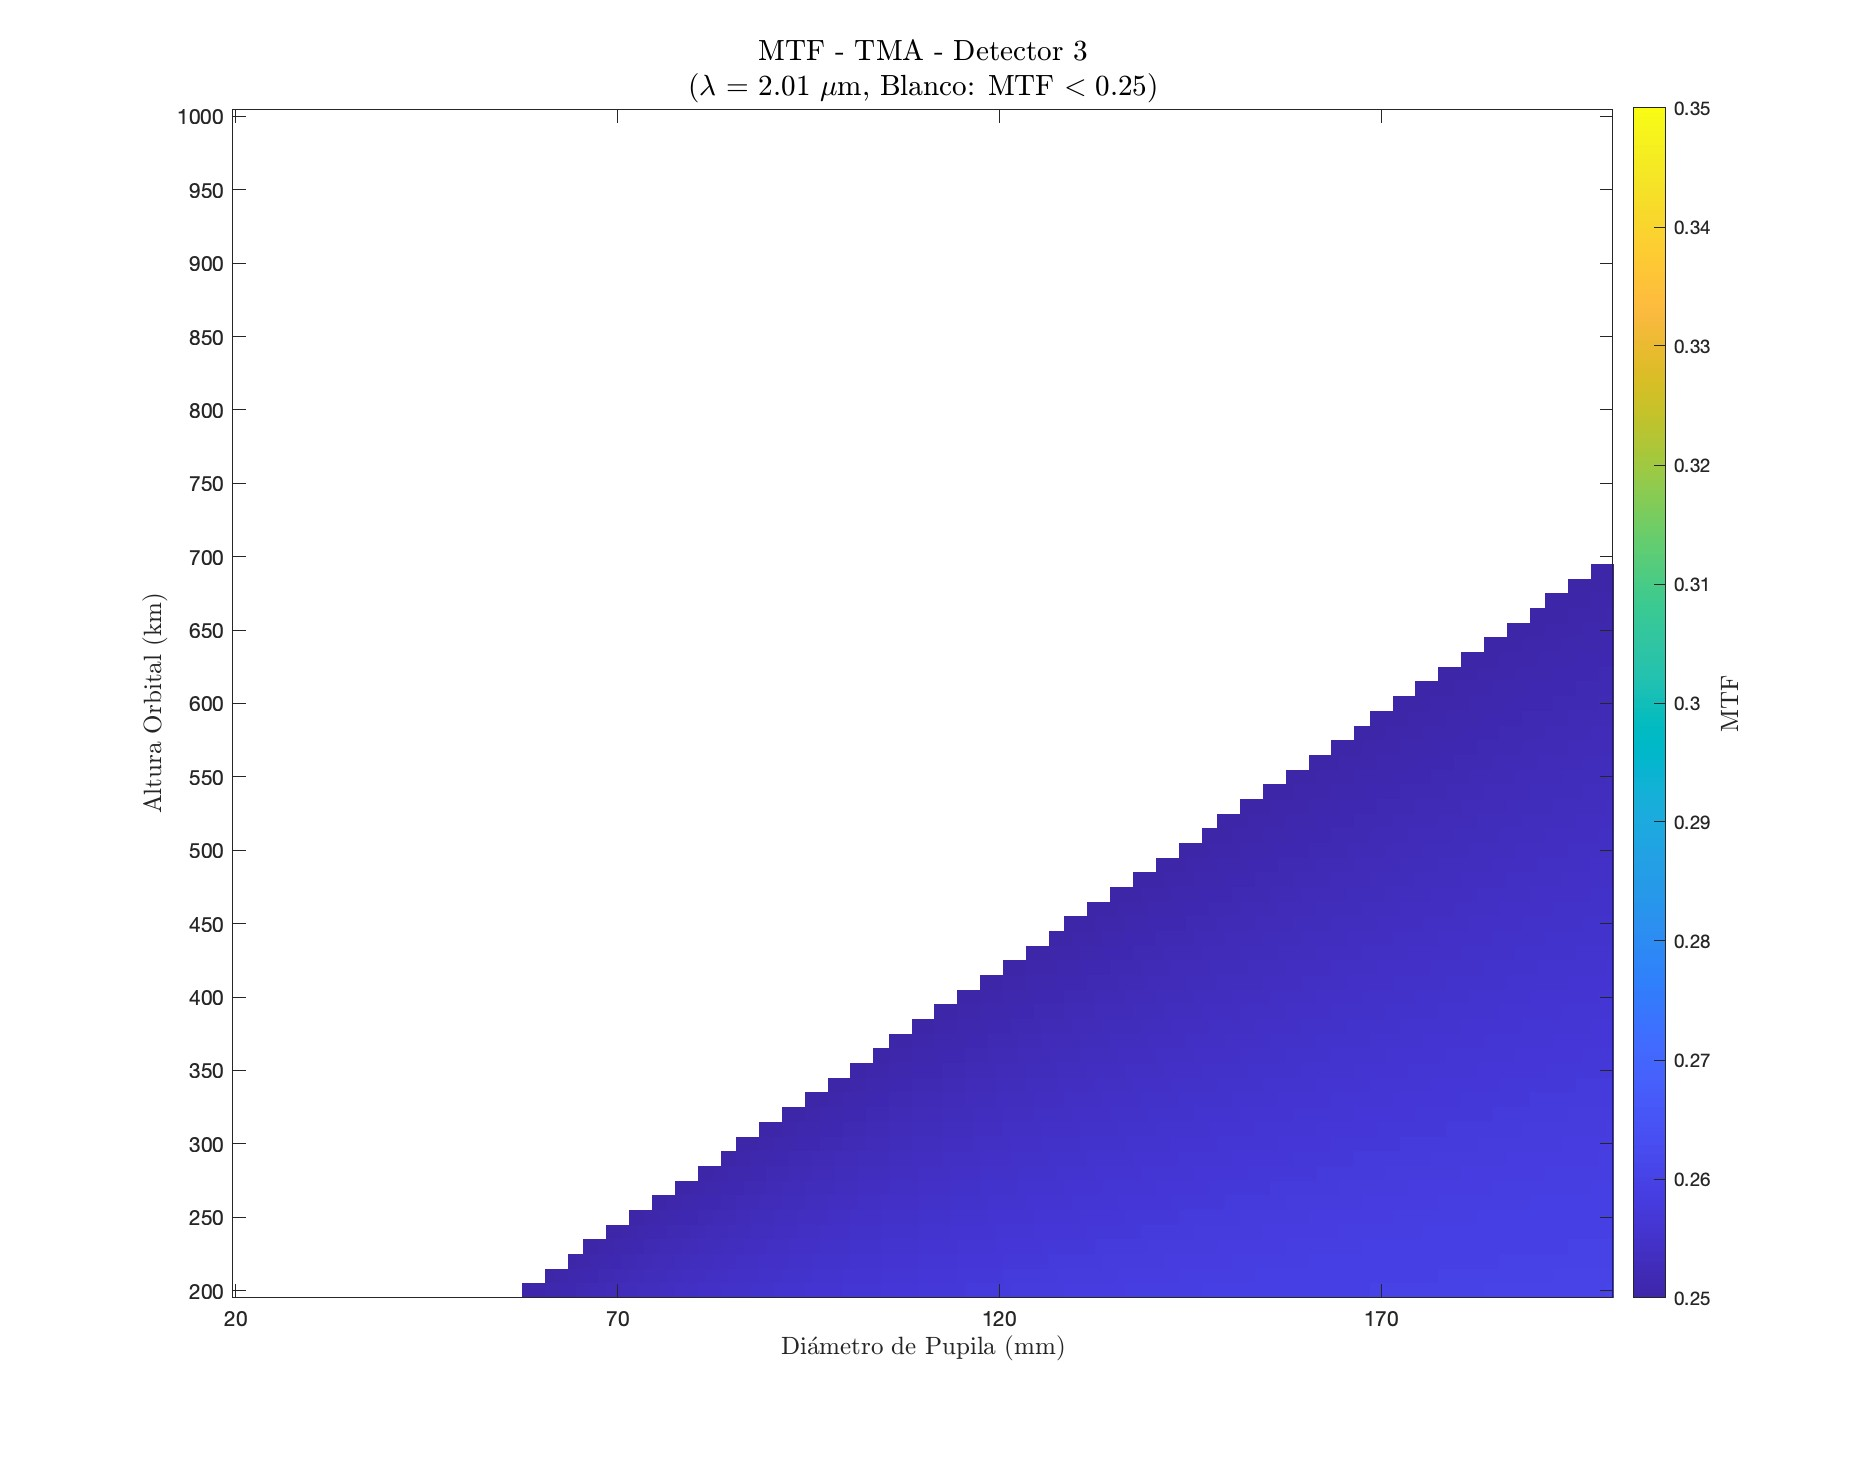
\includegraphics[width=0.48\linewidth]{4.Payload/MTF/MTF_Lambda2_Detector3_Telescopio4_heatmap.jpg} \\
\end{tabular}
\caption{Mapas de calor resultantes del calculo de MTF: Banda 2,01 \textmu m; Detector 3}
\end{figure}
\end{landscape}

Estos gráficos permiten extraer las siguientes consideraciones:

\begin{itemize}
    \item Como se aprecia, es un requisito que impone limitaciones considerables al diseño. No obstante, todavía aloja un espacio de diseño muy amplio, pues la única combinación no viable resulta en el detector 1 combinado con el telescopio TMA.
    \item El rendimiento más bajo, aunque con soluciones viables, es el detector 1, pues su MTF es la menor.
    \item De igual manera, es esperable, debido al alineamiento, que el telescopio con mejor rendimiento sea el refractivo, mientras el más pobre resulte el TMA.
\end{itemize}

\section{Cálculo de la SNR}

El cálculo de la relación señal-ruido (SNR) se ha realizado empleando las ecuaciones de la sección \ref{snr}. Para cada combinación de diámetro de pupila y altura orbital, y considerando los diferentes detectores y tipos de telescopio, se han generado mapas de calor que representan los valores de SNR obtenidos.

En este análisis se han utilizado los parámetro expuestos de detectores (tablas \ref{tab:detectores_comparacion_2}) y de telescopios(tabla \ref{tab:tabla_telescopios}), así como los parámetros iniciales especificados en la tabla \ref{initialsnr}, que incluyen tanto las características instrumentales como los valores de ruido en condiciones de peor caso. Este enfoque permite identificar, para cada configuración, las regiones del espacio de diseño que cumplen con los requisitos mínimos de SNR establecidos para la misión.


\begin{table}[H]
\centering
\caption{Parámetros iniciales y fuentes de ruido para el cálculo de SNR}
\begin{tabular}{l r}
\hline
\multicolumn{2}{c}{\textbf{Parámetros iniciales}} \\
\hline
TDI & 1\tablefootnote{un TDI=1 equivale a no implementado.} \\
Radiancia de referencia & 100 W/m\textsuperscript{2}·sr·\textmu m \\
\hline
\multicolumn{2}{c}{\textbf{Ruidos}\cite{gravrand_development_2017}} \\
\hline
$N_{dark}$ & 50 $e^-$  \\
$N_{read}$ & 100 $e^-$  \\
$N_{preamp}$ & 5 $e^-$  \\
$N_{video}$ & 10 $e^-$  \\
$N_{jitter}$ & 5 $e^-$  \\
$N_{emc}$ & 5 $e^-$  \\
$N_{quant}$ & 2 $e^-$  \\
$N_{nonlin}$ & 2 $e^-$  \\
\hline
\label{initialsnr}
\end{tabular}

\label{tab:parametros_ruidos}
\end{table}

De igual manera que en la computación del MTF total, se añade al \textbf{SNR un margen del 10\%} en calidad de reserva de diseño. En las etapas iniciales, los parámetros contribuyentes experimentan variaciones que pueden degradar el rendimiento del sistema. Este margen de seguridad permite absorber dichas desviaciones y garantizar el cumplimiento de los requisitos establecidos.

De nuevo, solo se presenta la banda más restrictiva. En este caso, será la de menor longitud de onda: la banda $0,76 \mu m$, ya que la longitud de onda es directamente proporcional a la irradiancia, y por ello, al número de electrones que recibe el detector. El resto se encuentran de nuevo en el anexo \ref{sec:annexdata}. A continuación se presentan las gráficas correspondientes, que muestran la variación de la SNR en función del diámetro de pupila y la altura orbital para las distintas opciones de detectores y telescopios evaluados:

%% GRAFICAS SNR

%% Lambda 3

\begin{landscape}
\begin{figure}[p]
\centering
\vspace*{0.3cm}


\vspace{0.3cm}
\setlength{\tabcolsep}{4pt}
\renewcommand{\arraystretch}{0}

\begin{tabular}{cc}
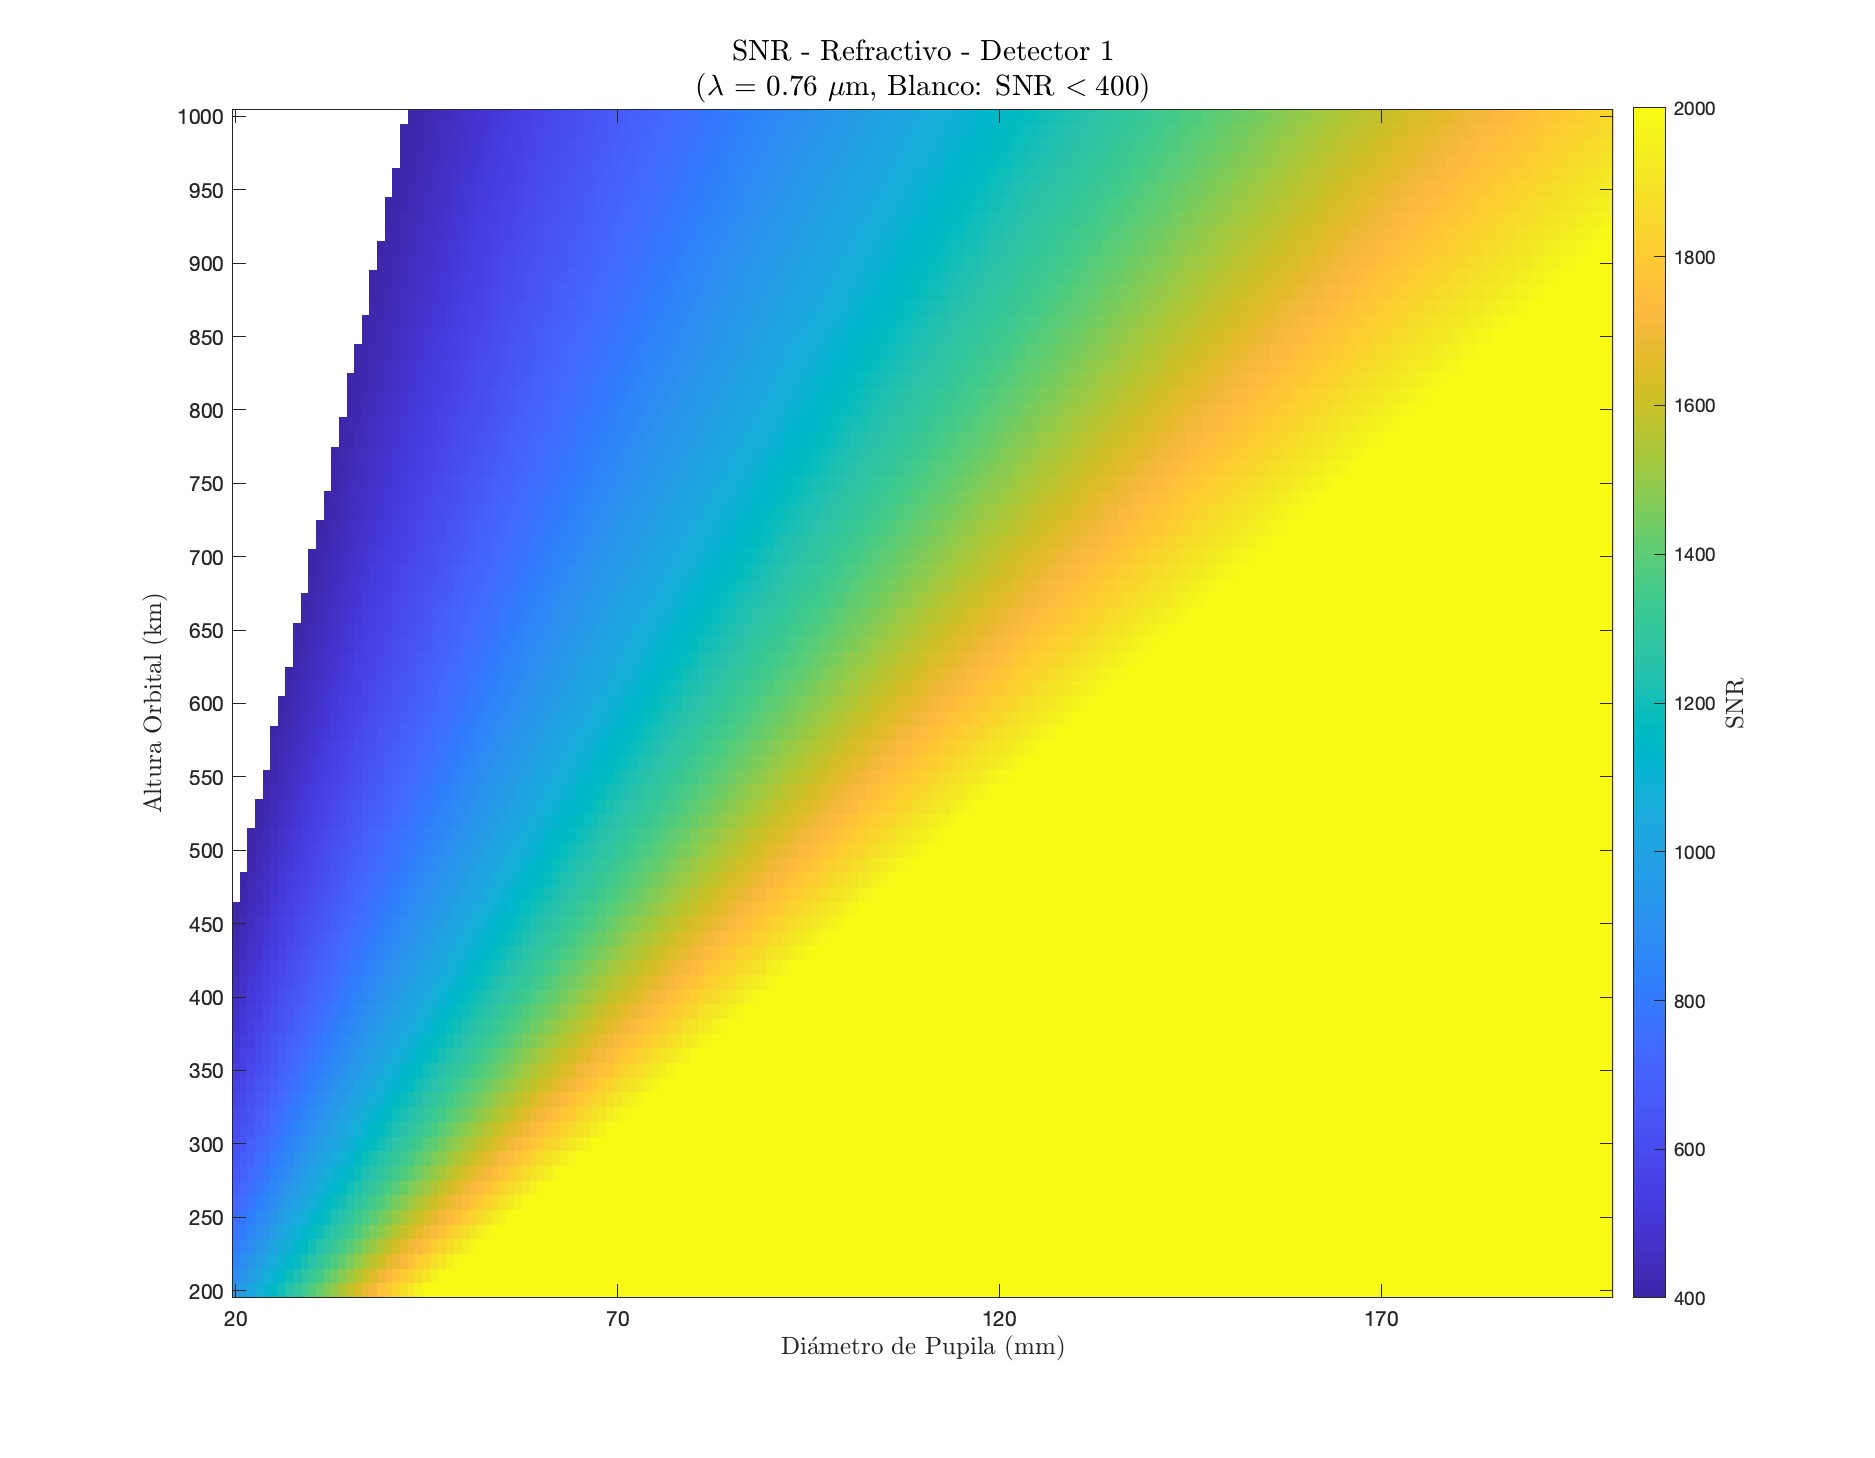
\includegraphics[width=0.48\linewidth]{4.Payload/SNR/SNR_Lambda3_Detector4_Telescopio1_heatmap.jpg} &
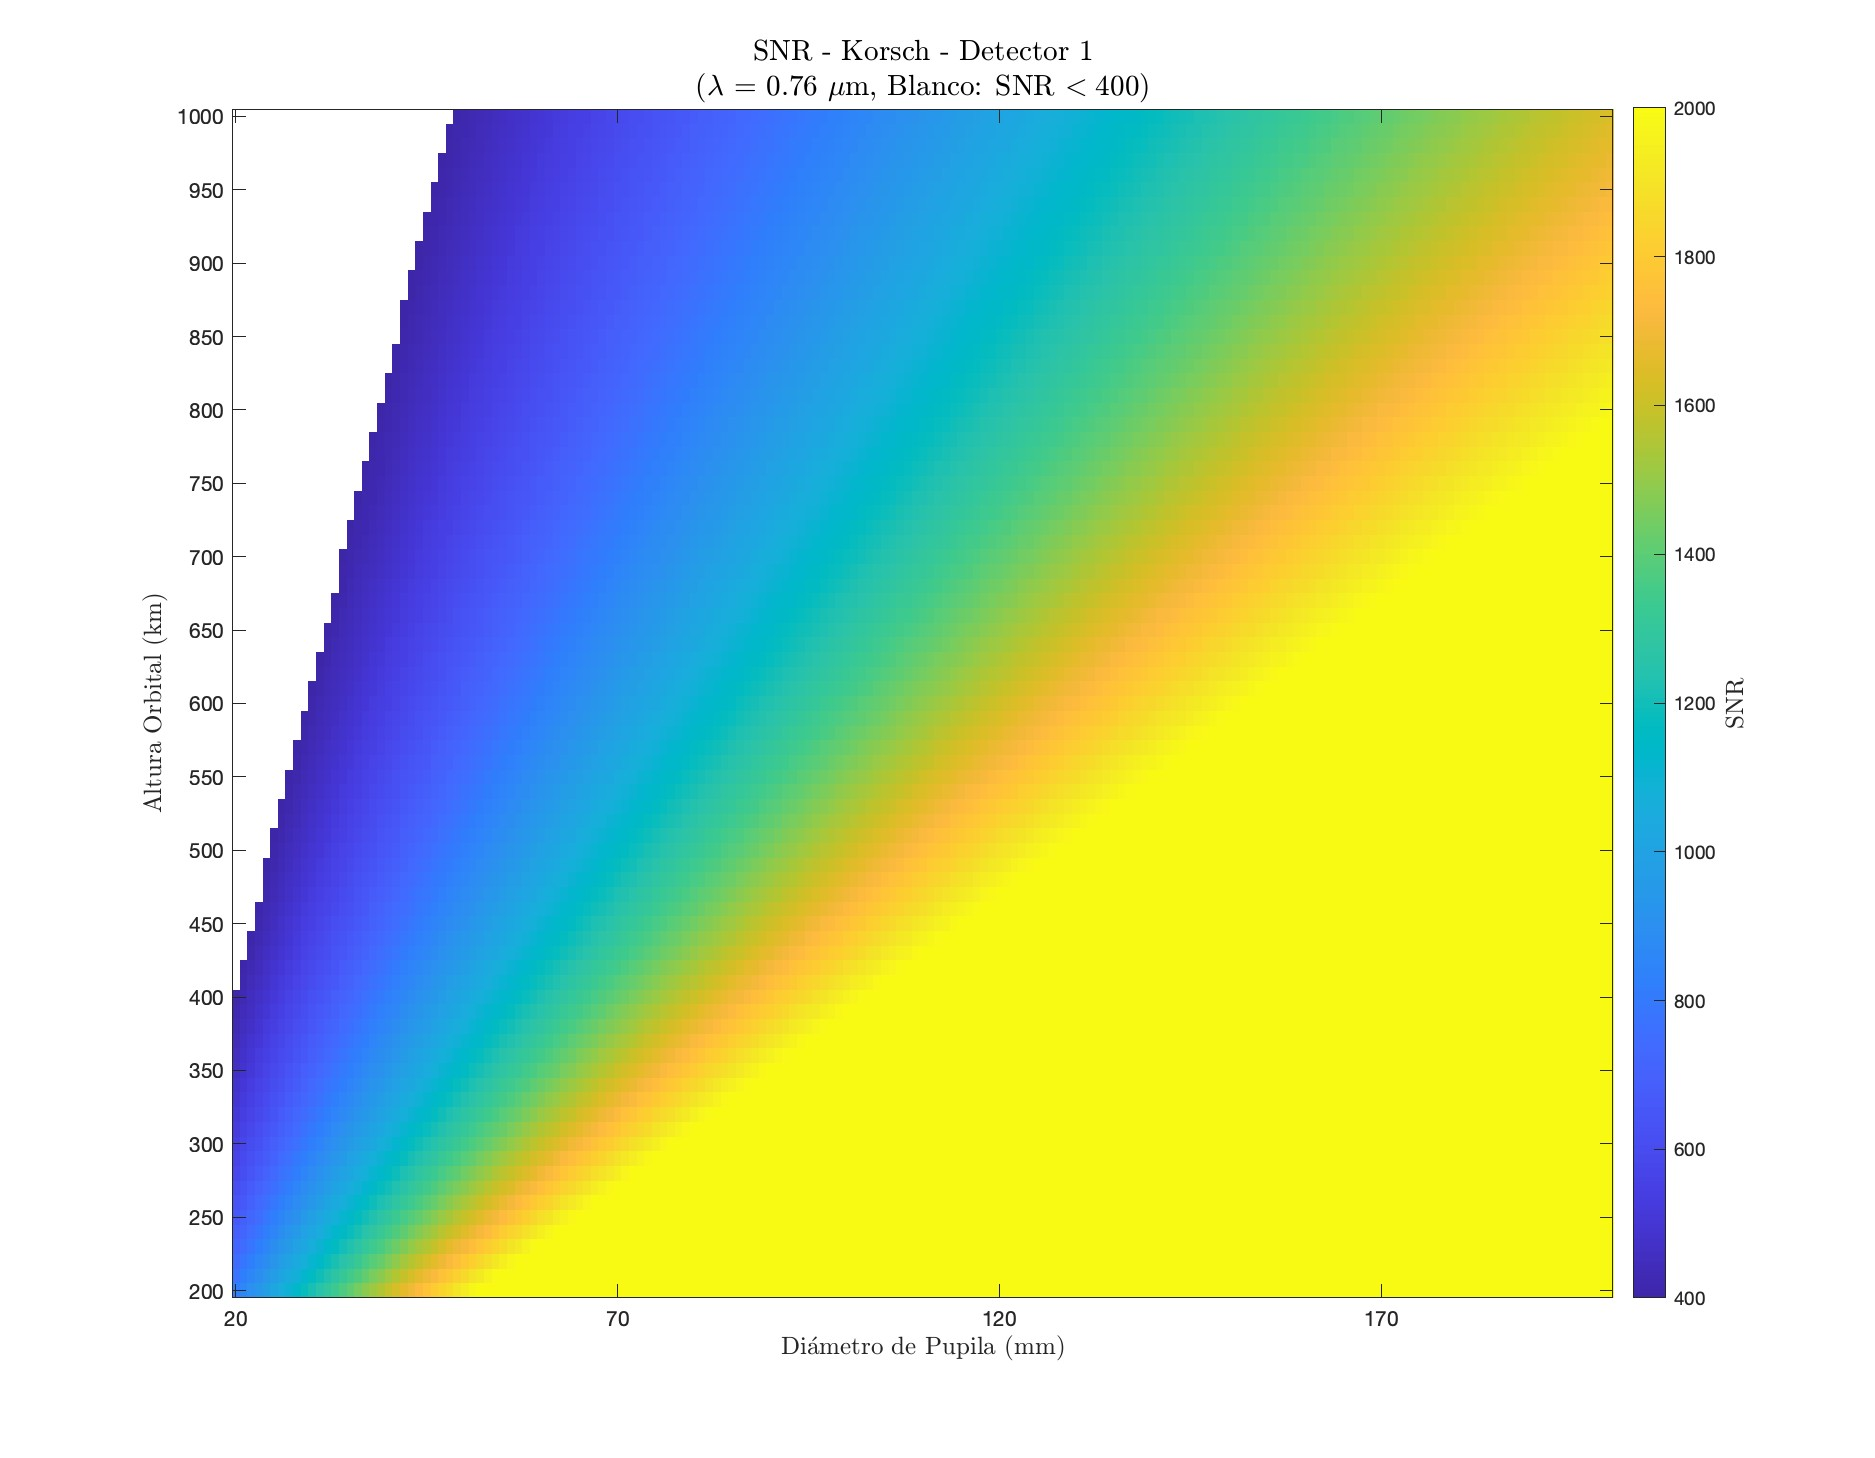
\includegraphics[width=0.48\linewidth]{4.Payload/SNR/SNR_Lambda3_Detector4_Telescopio2_heatmap.jpg} \\
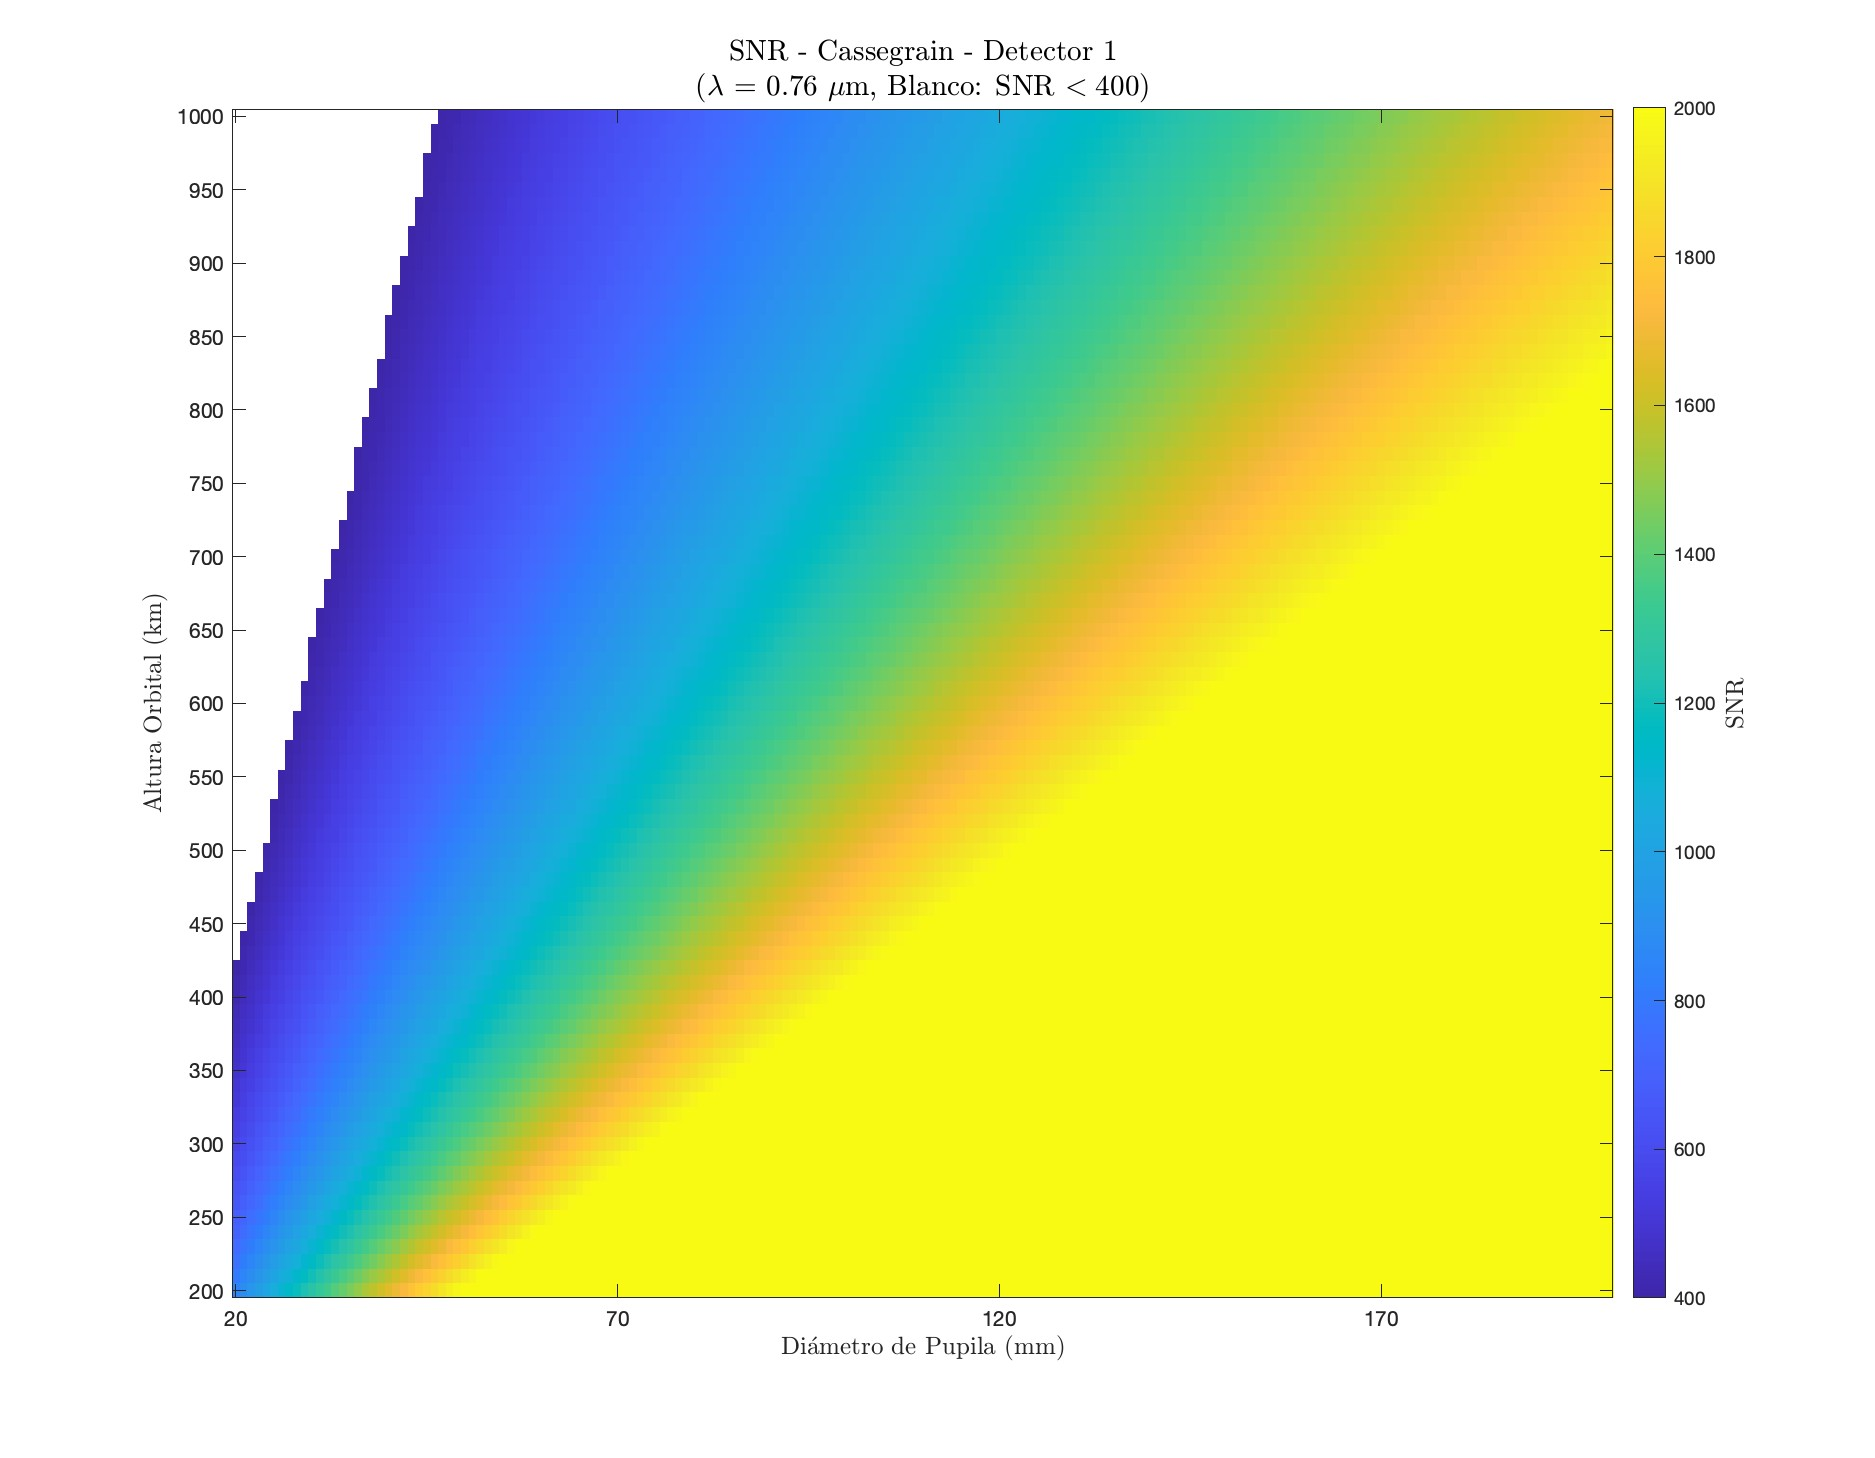
\includegraphics[width=0.48\linewidth]{4.Payload/SNR/SNR_Lambda3_Detector4_Telescopio3_heatmap.jpg} &
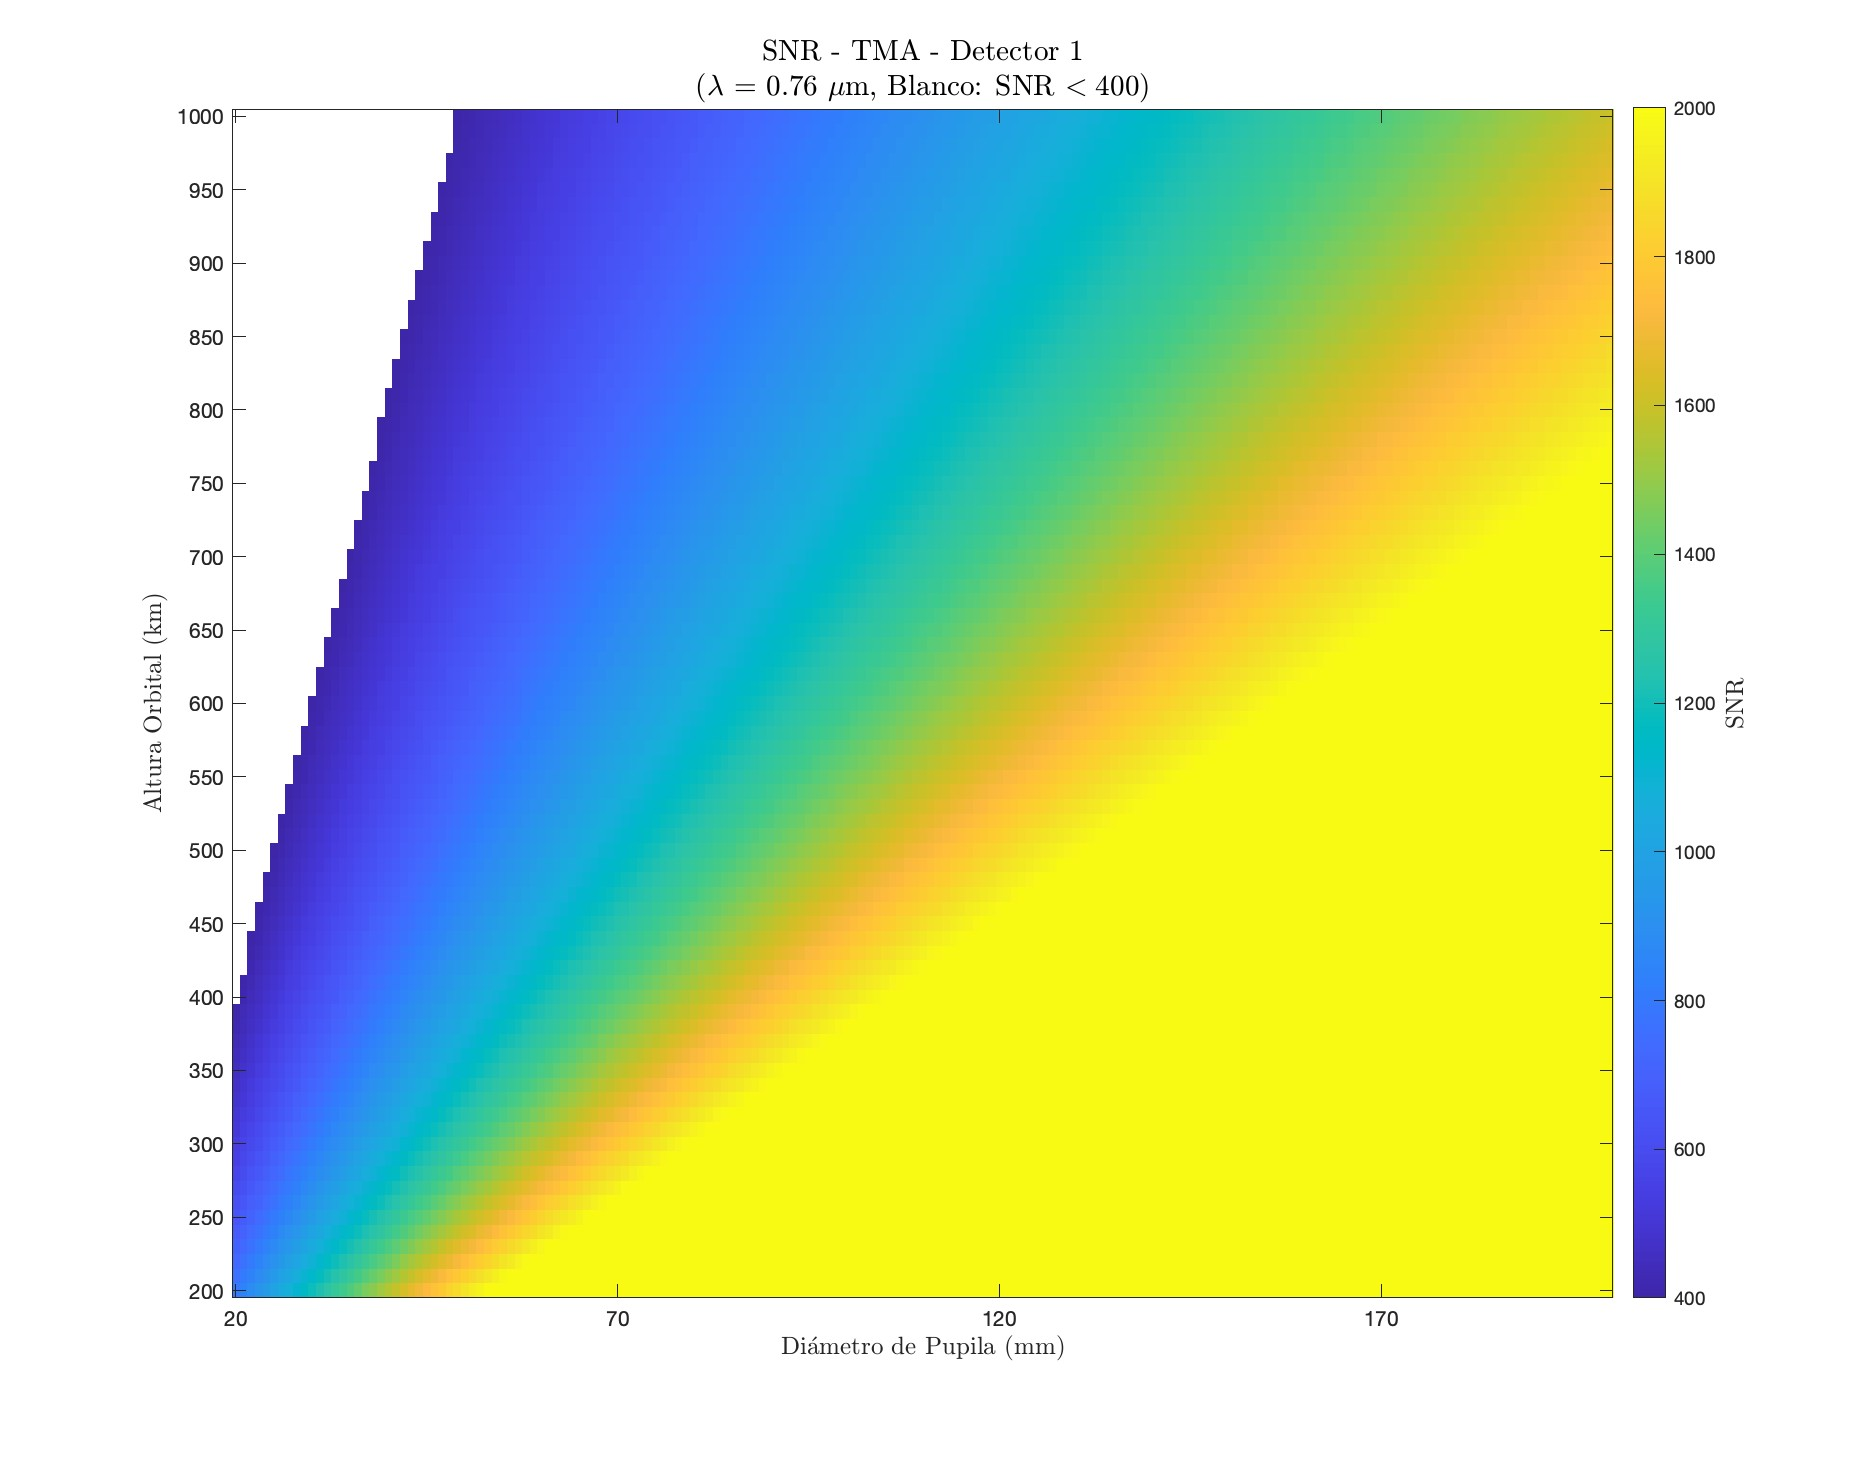
\includegraphics[width=0.48\linewidth]{4.Payload/SNR/SNR_Lambda3_Detector4_Telescopio4_heatmap.jpg} \\
\end{tabular}
\caption{Mapas de calor resultantes del calculo de SNR: Banda 0,76 \textmu m; Detector 1}
\end{figure}
\end{landscape}

% Detector 2
\begin{landscape}
\begin{figure}[p]
\centering
\vspace*{0.3cm}

\vspace{0.3cm}
\setlength{\tabcolsep}{4pt}
\renewcommand{\arraystretch}{0}

\begin{tabular}{cc}
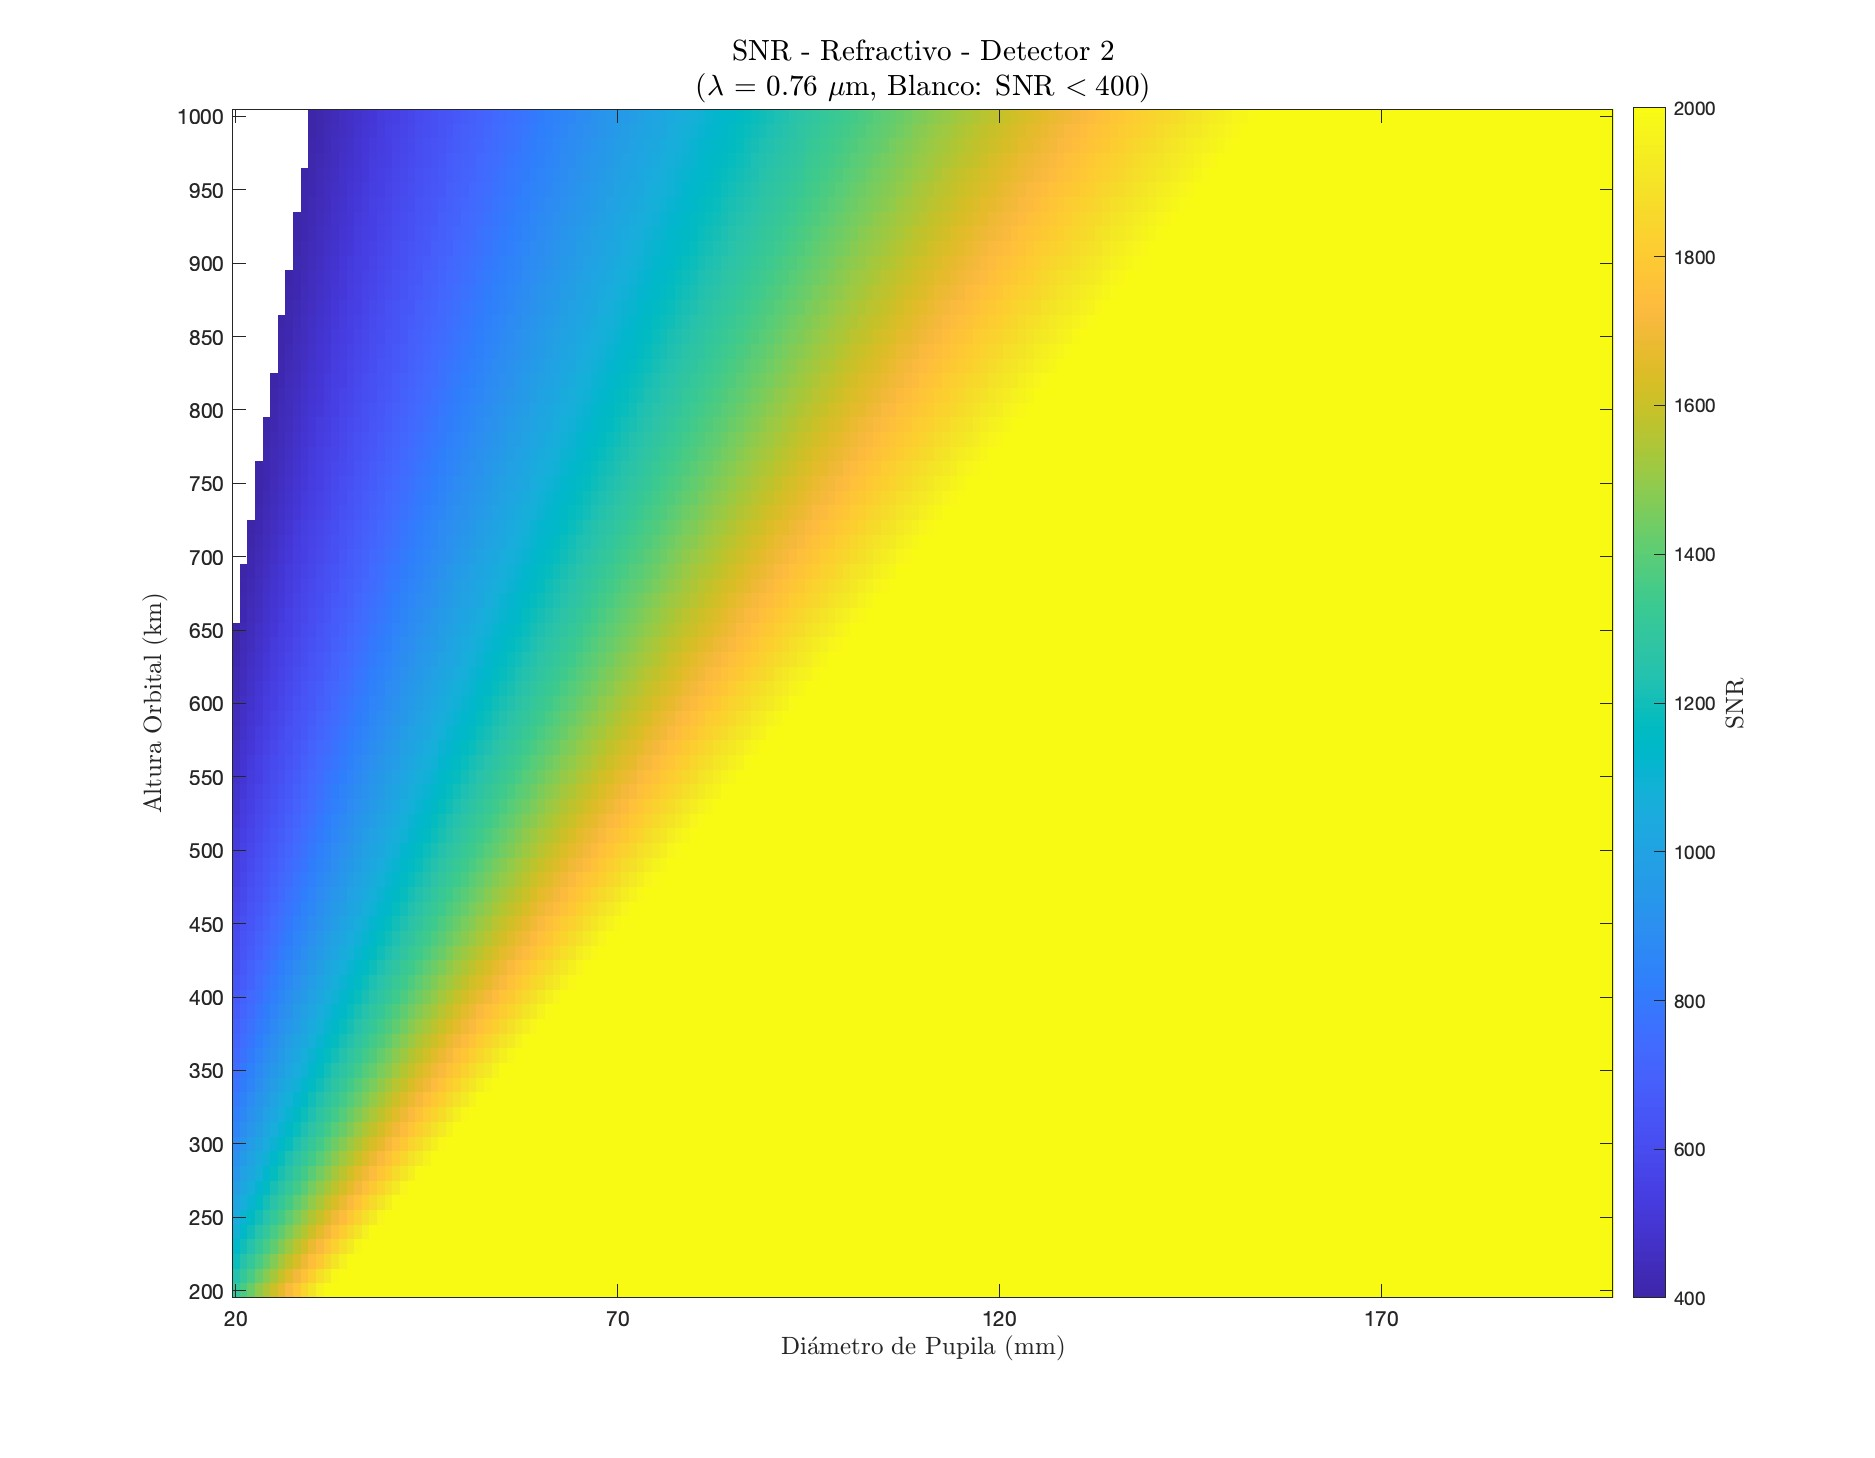
\includegraphics[width=0.48\linewidth]{4.Payload/SNR/SNR_Lambda3_Detector5_Telescopio1_heatmap.jpg} &
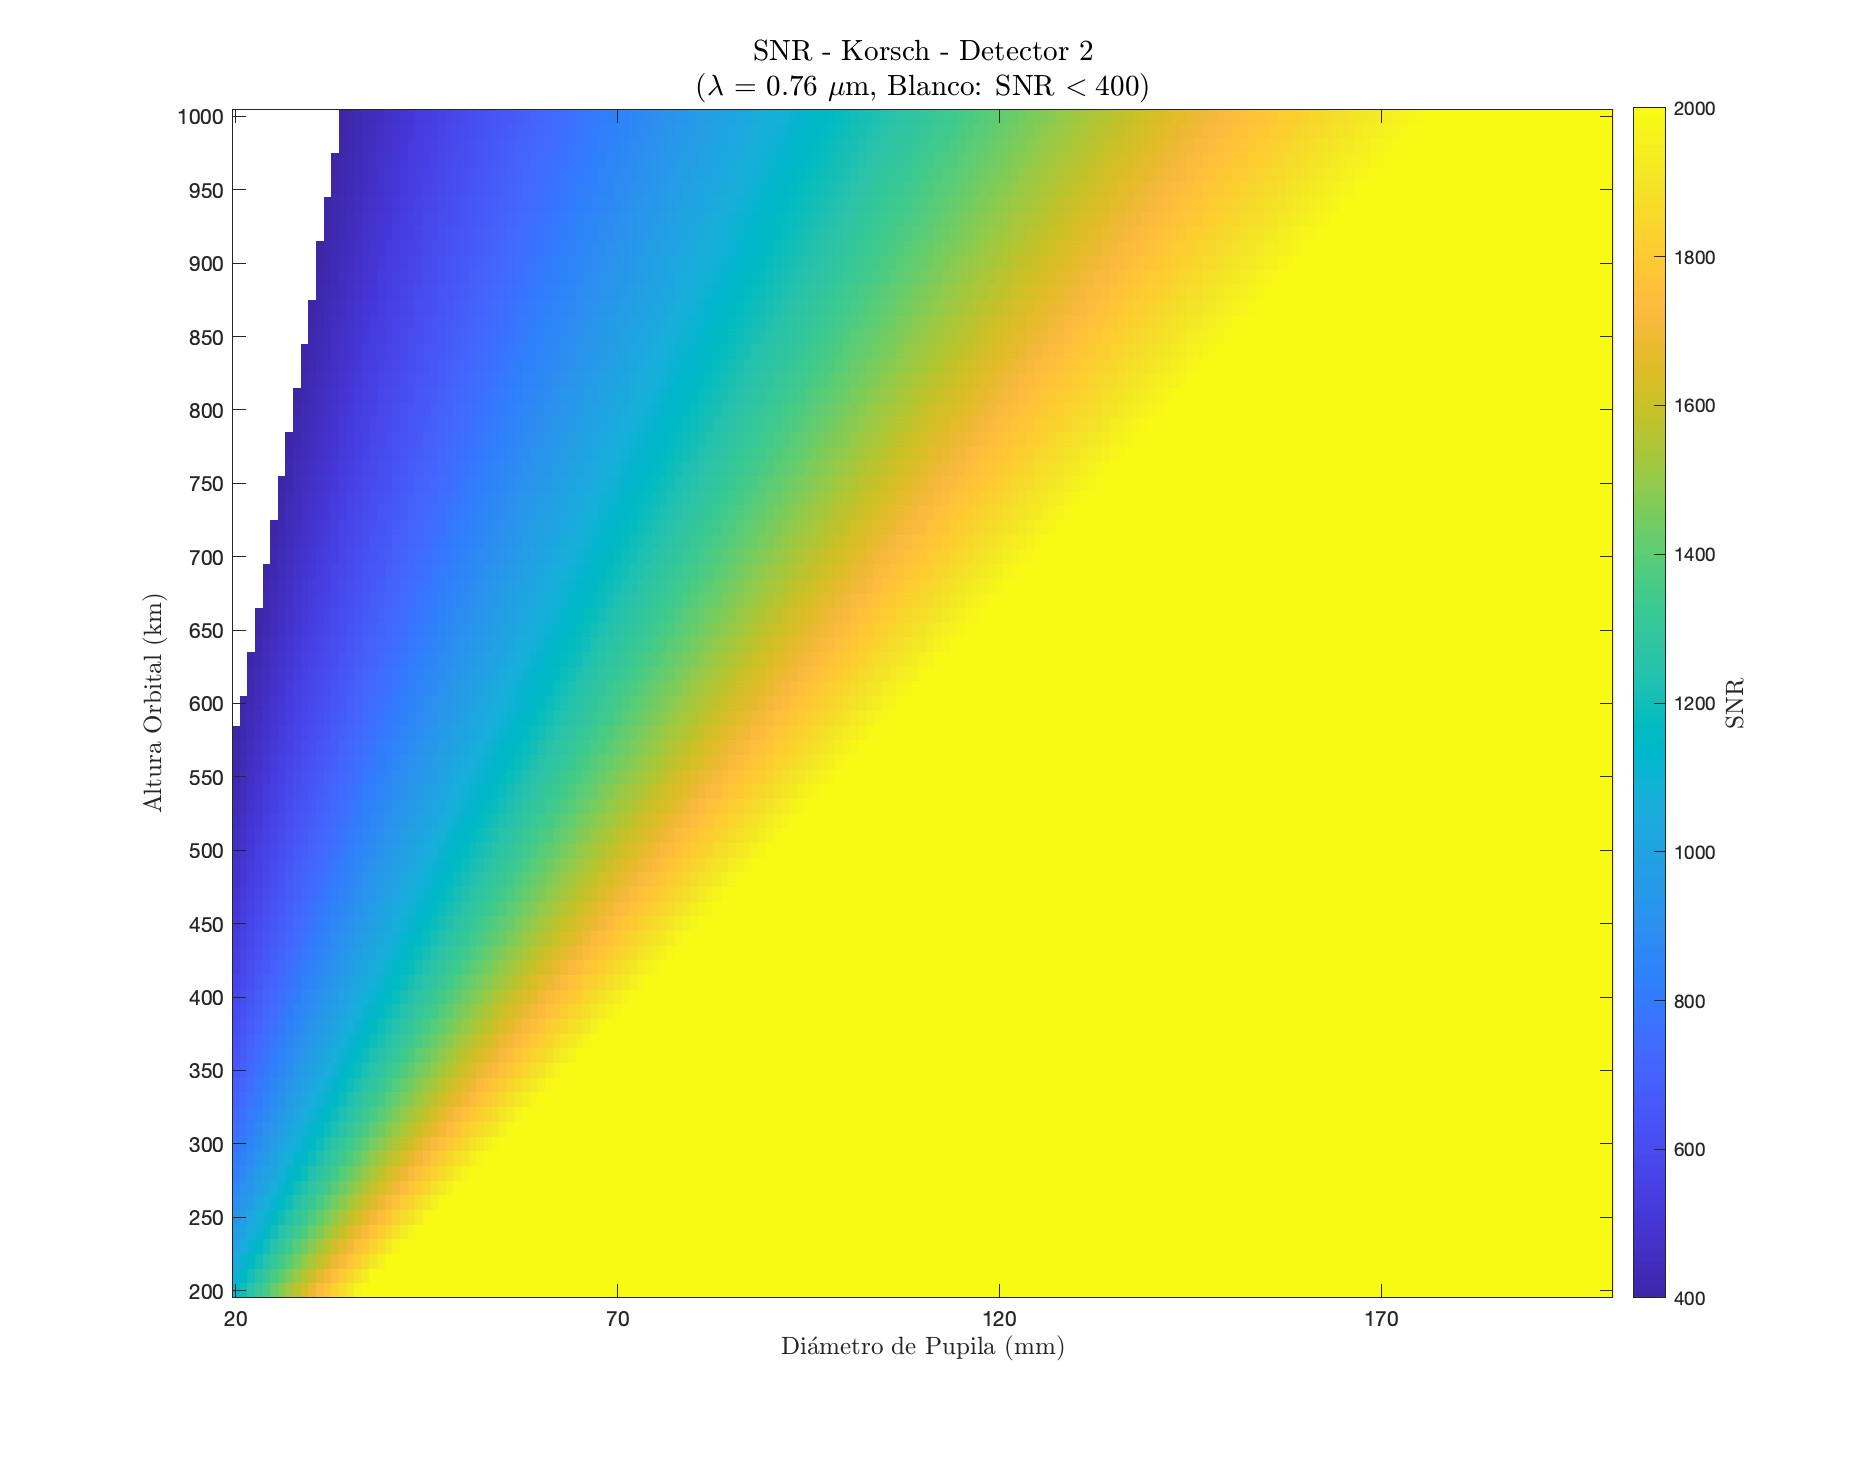
\includegraphics[width=0.48\linewidth]{4.Payload/SNR/SNR_Lambda3_Detector5_Telescopio2_heatmap.jpg} \\
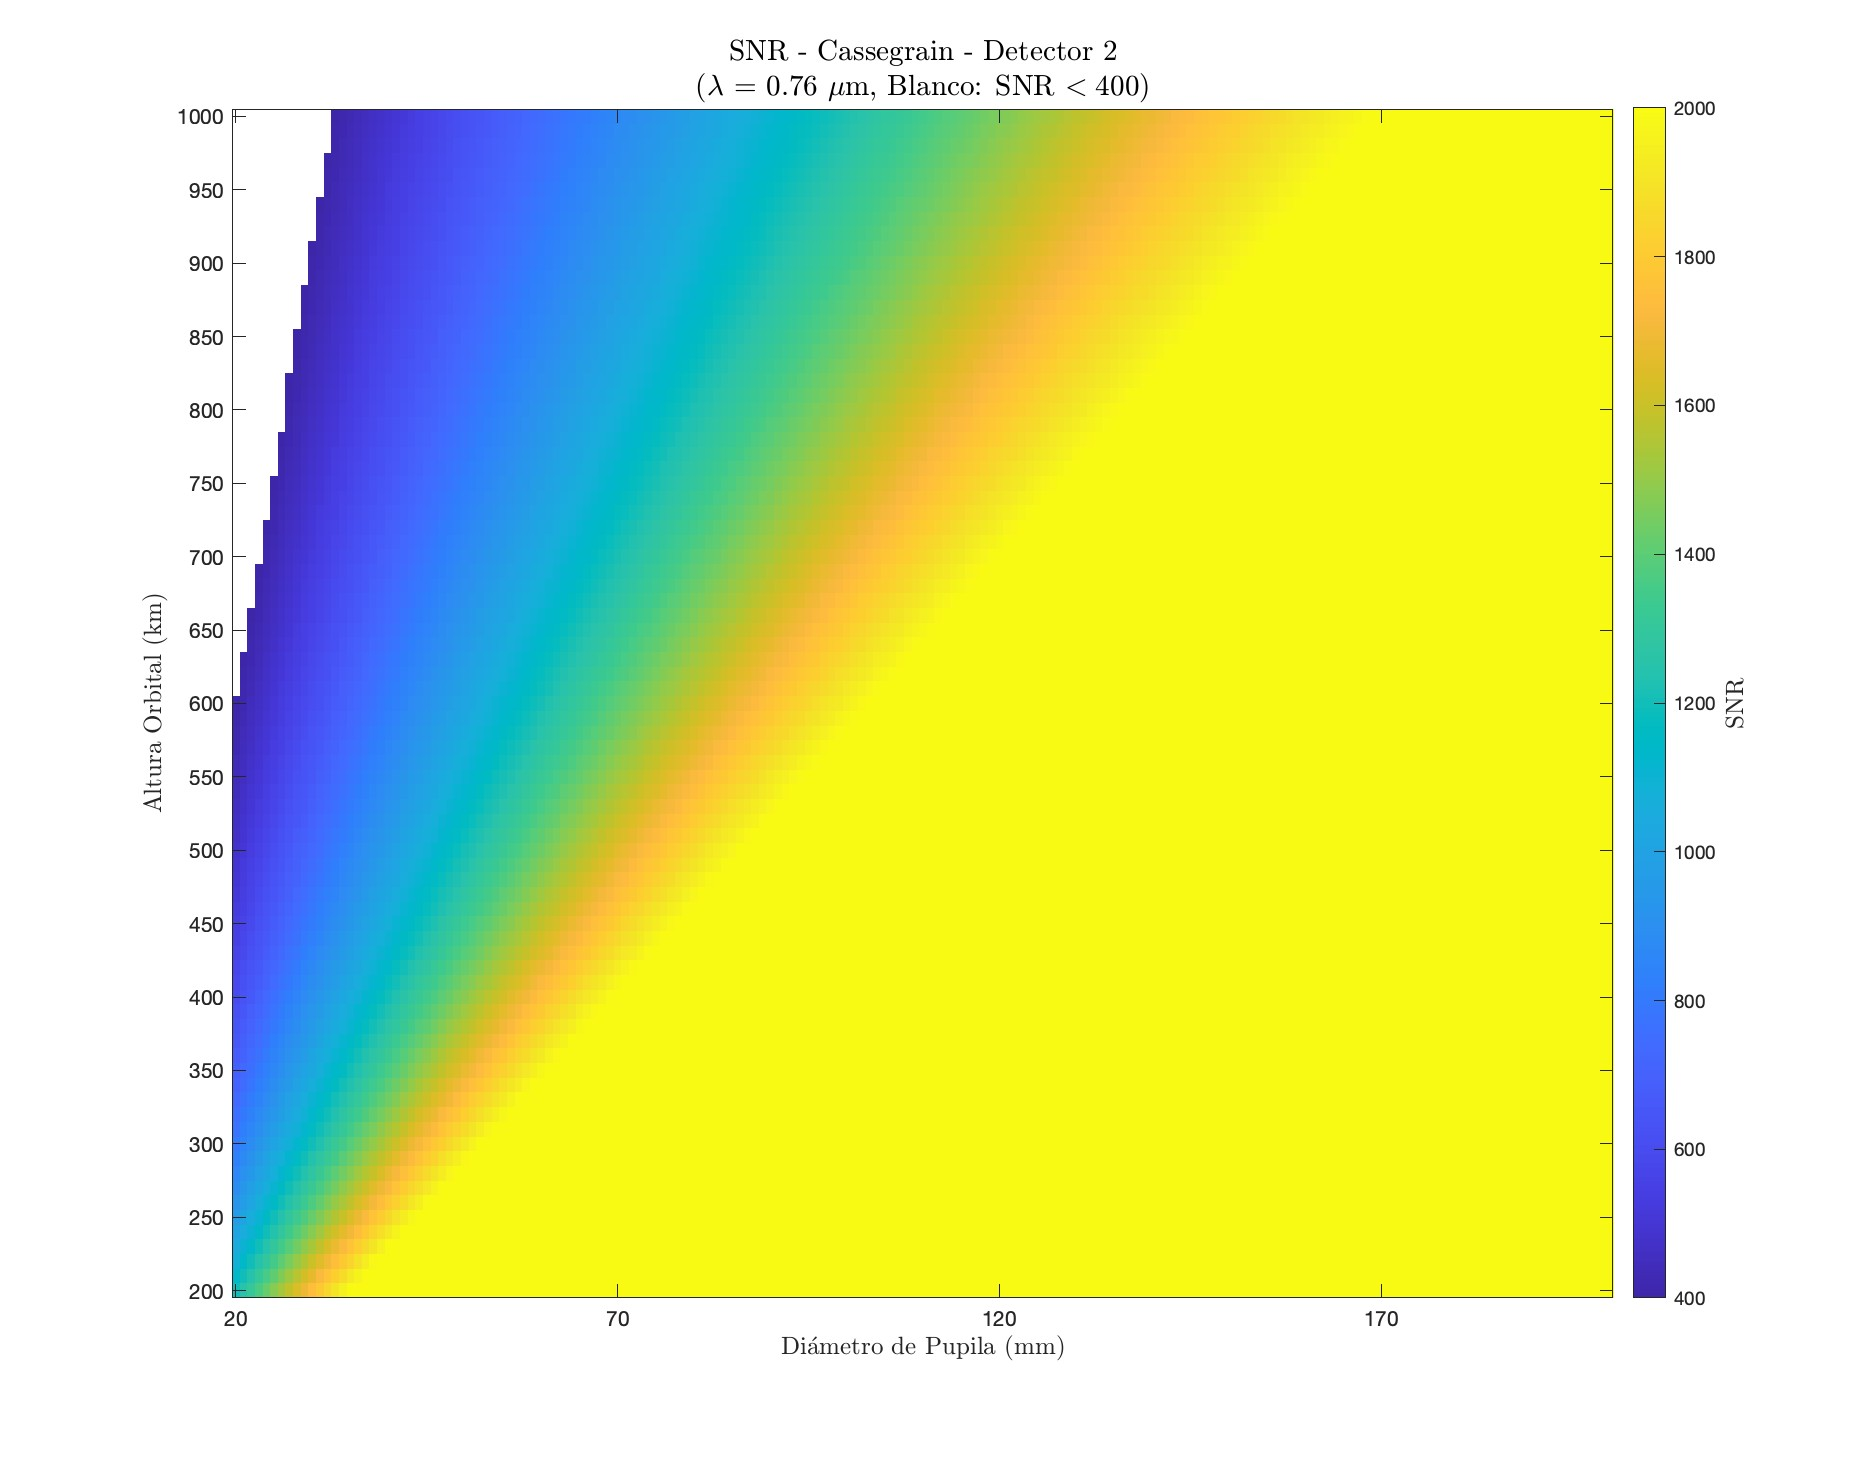
\includegraphics[width=0.48\linewidth]{4.Payload/SNR/SNR_Lambda3_Detector5_Telescopio3_heatmap.jpg} &
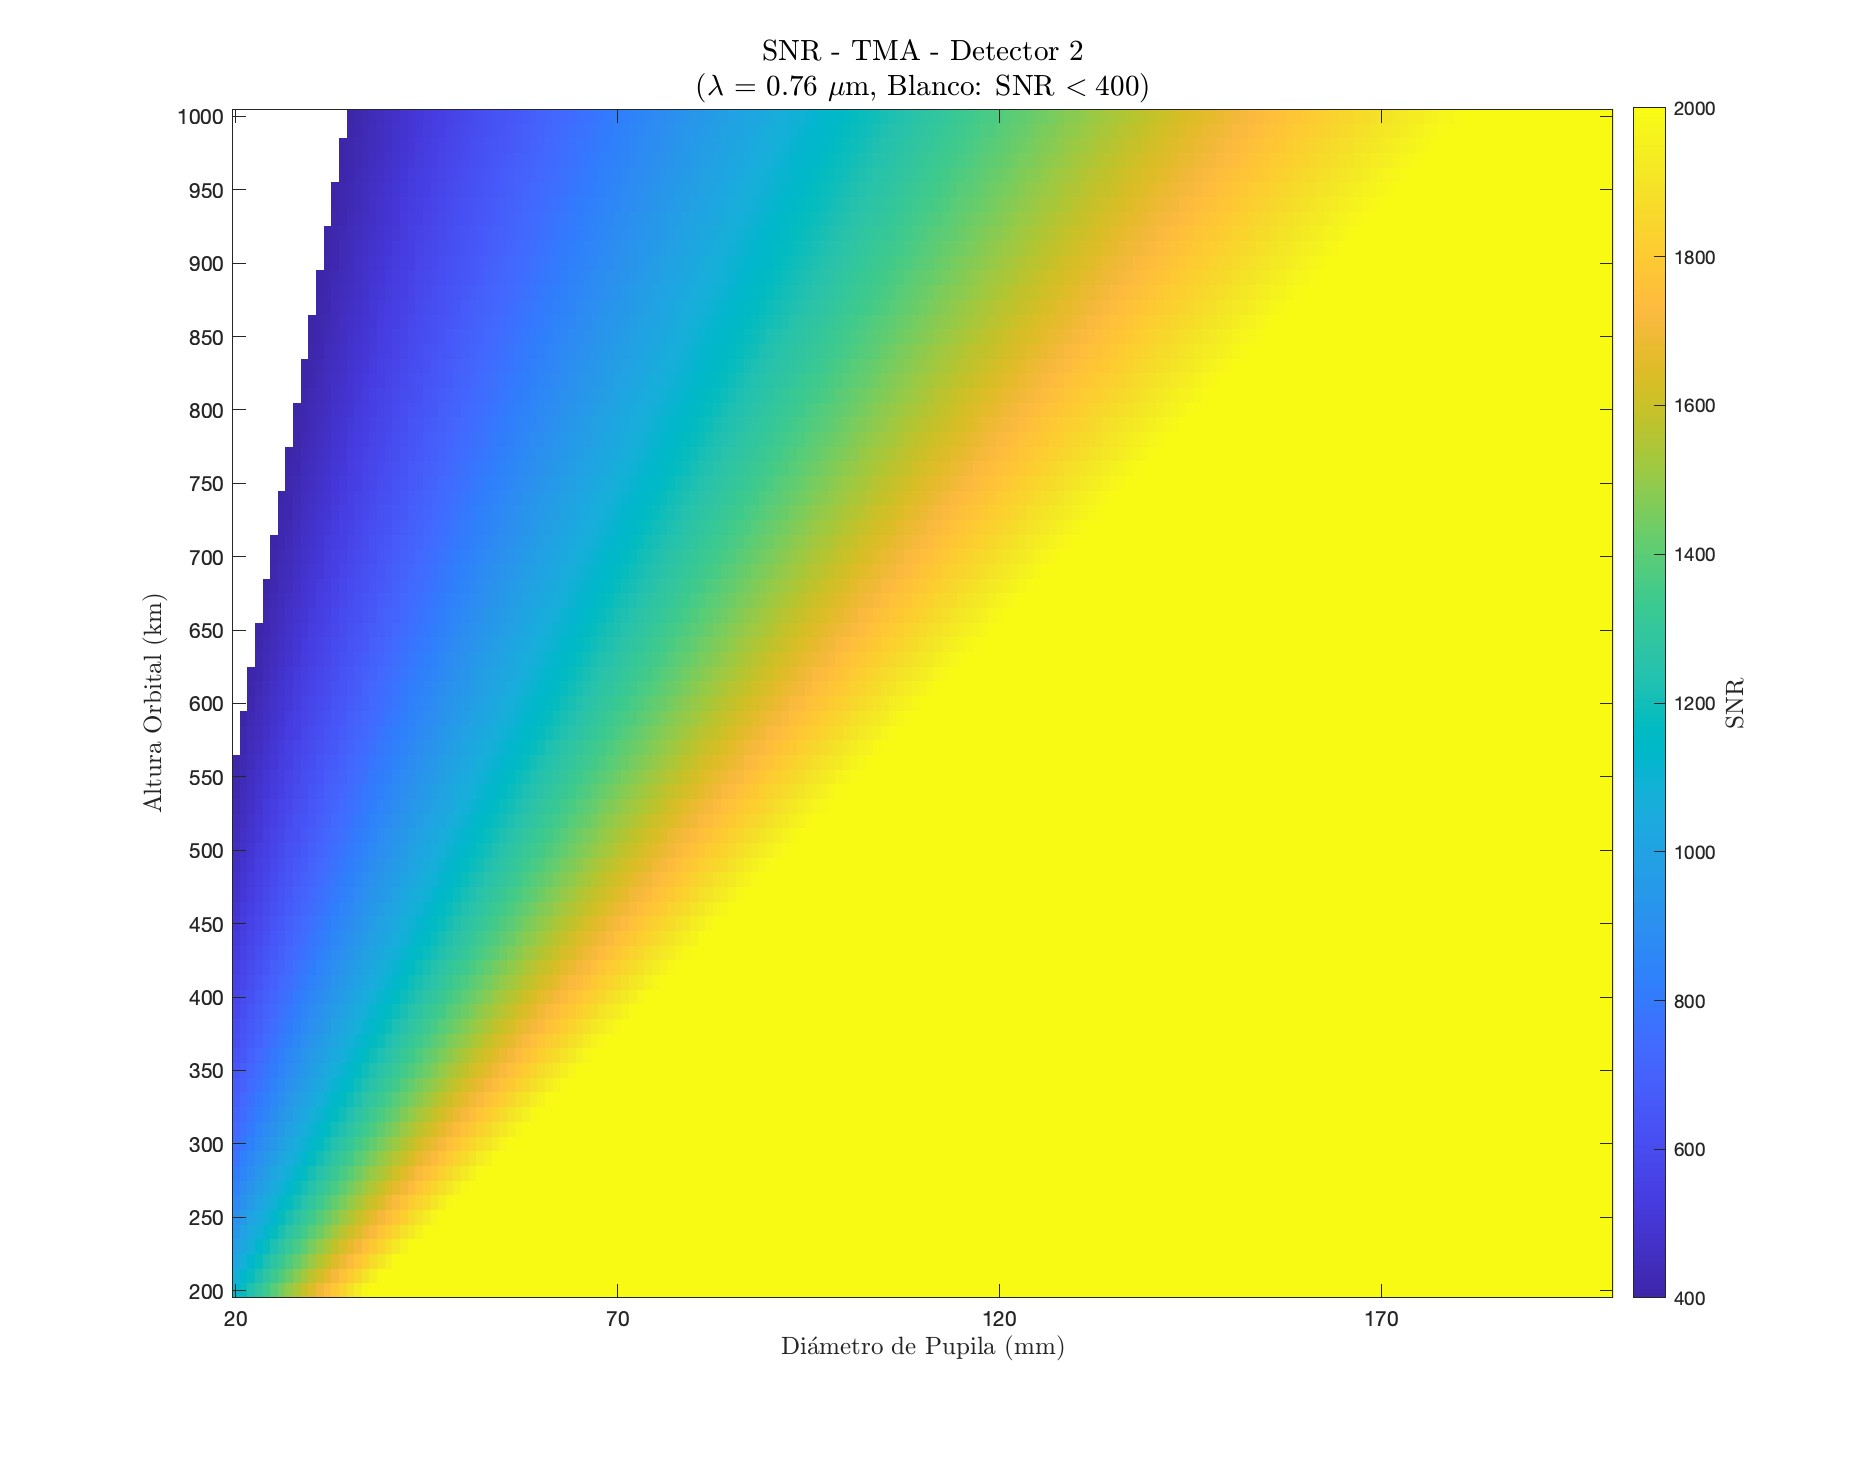
\includegraphics[width=0.48\linewidth]{4.Payload/SNR/SNR_Lambda3_Detector5_Telescopio4_heatmap.jpg} \\
\end{tabular}
\caption{Mapas de calor resultantes del calculo de SNR: Banda 0,76 \textmu m; Detector 2}
\end{figure}
\end{landscape}

% Detector 3
\begin{landscape}
\begin{figure}[p]
\centering
\vspace*{0.3cm}

\vspace{0.3cm}
\setlength{\tabcolsep}{4pt}
\renewcommand{\arraystretch}{0}

\begin{tabular}{cc}
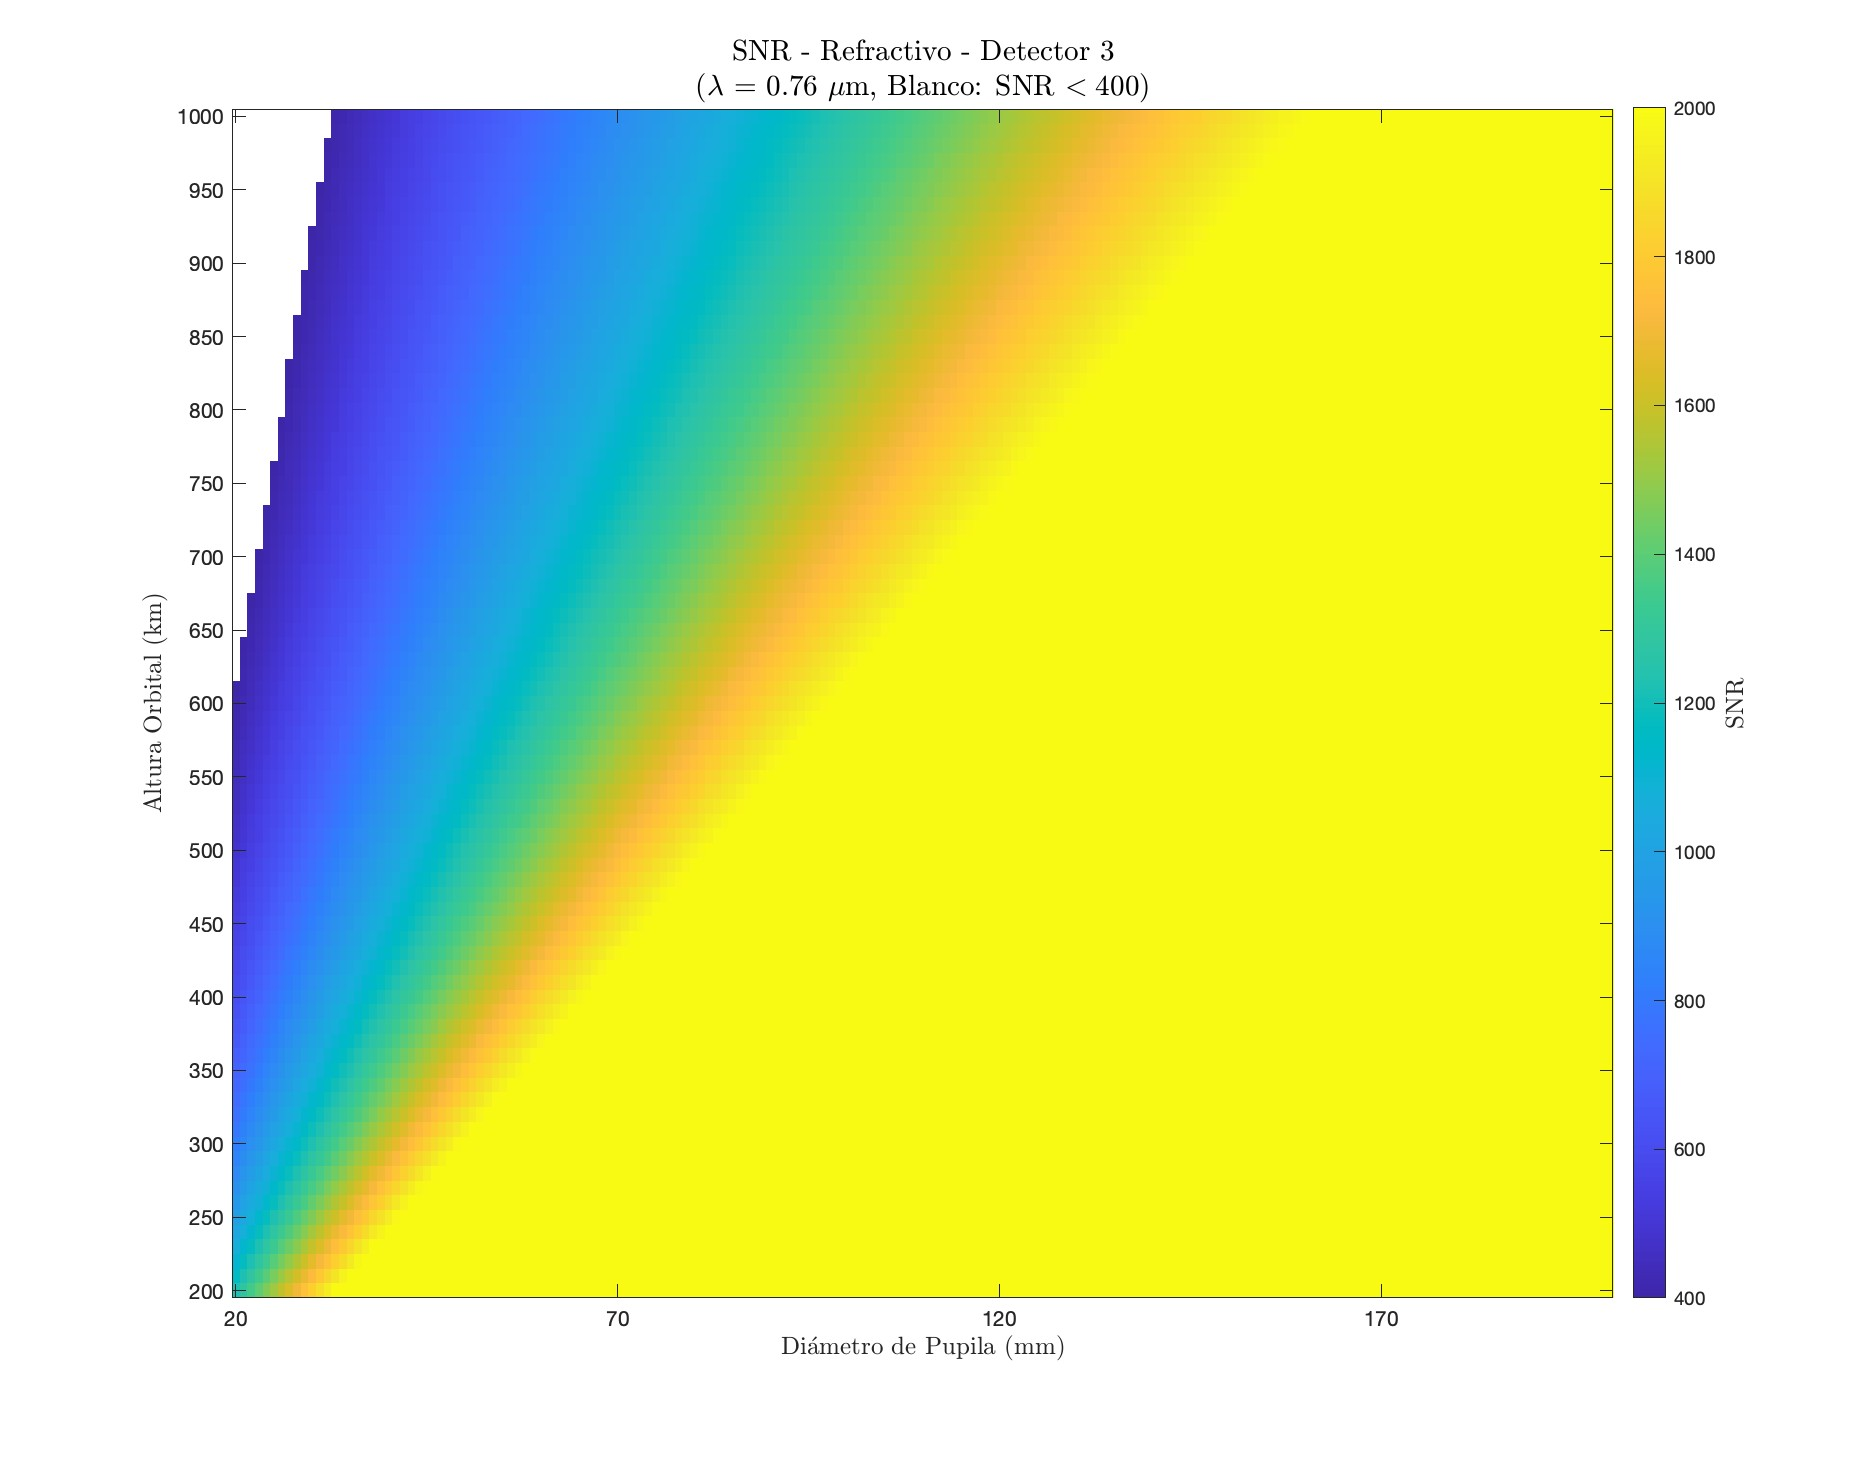
\includegraphics[width=0.48\linewidth]{4.Payload/SNR/SNR_Lambda3_Detector6_Telescopio1_heatmap.jpg} &
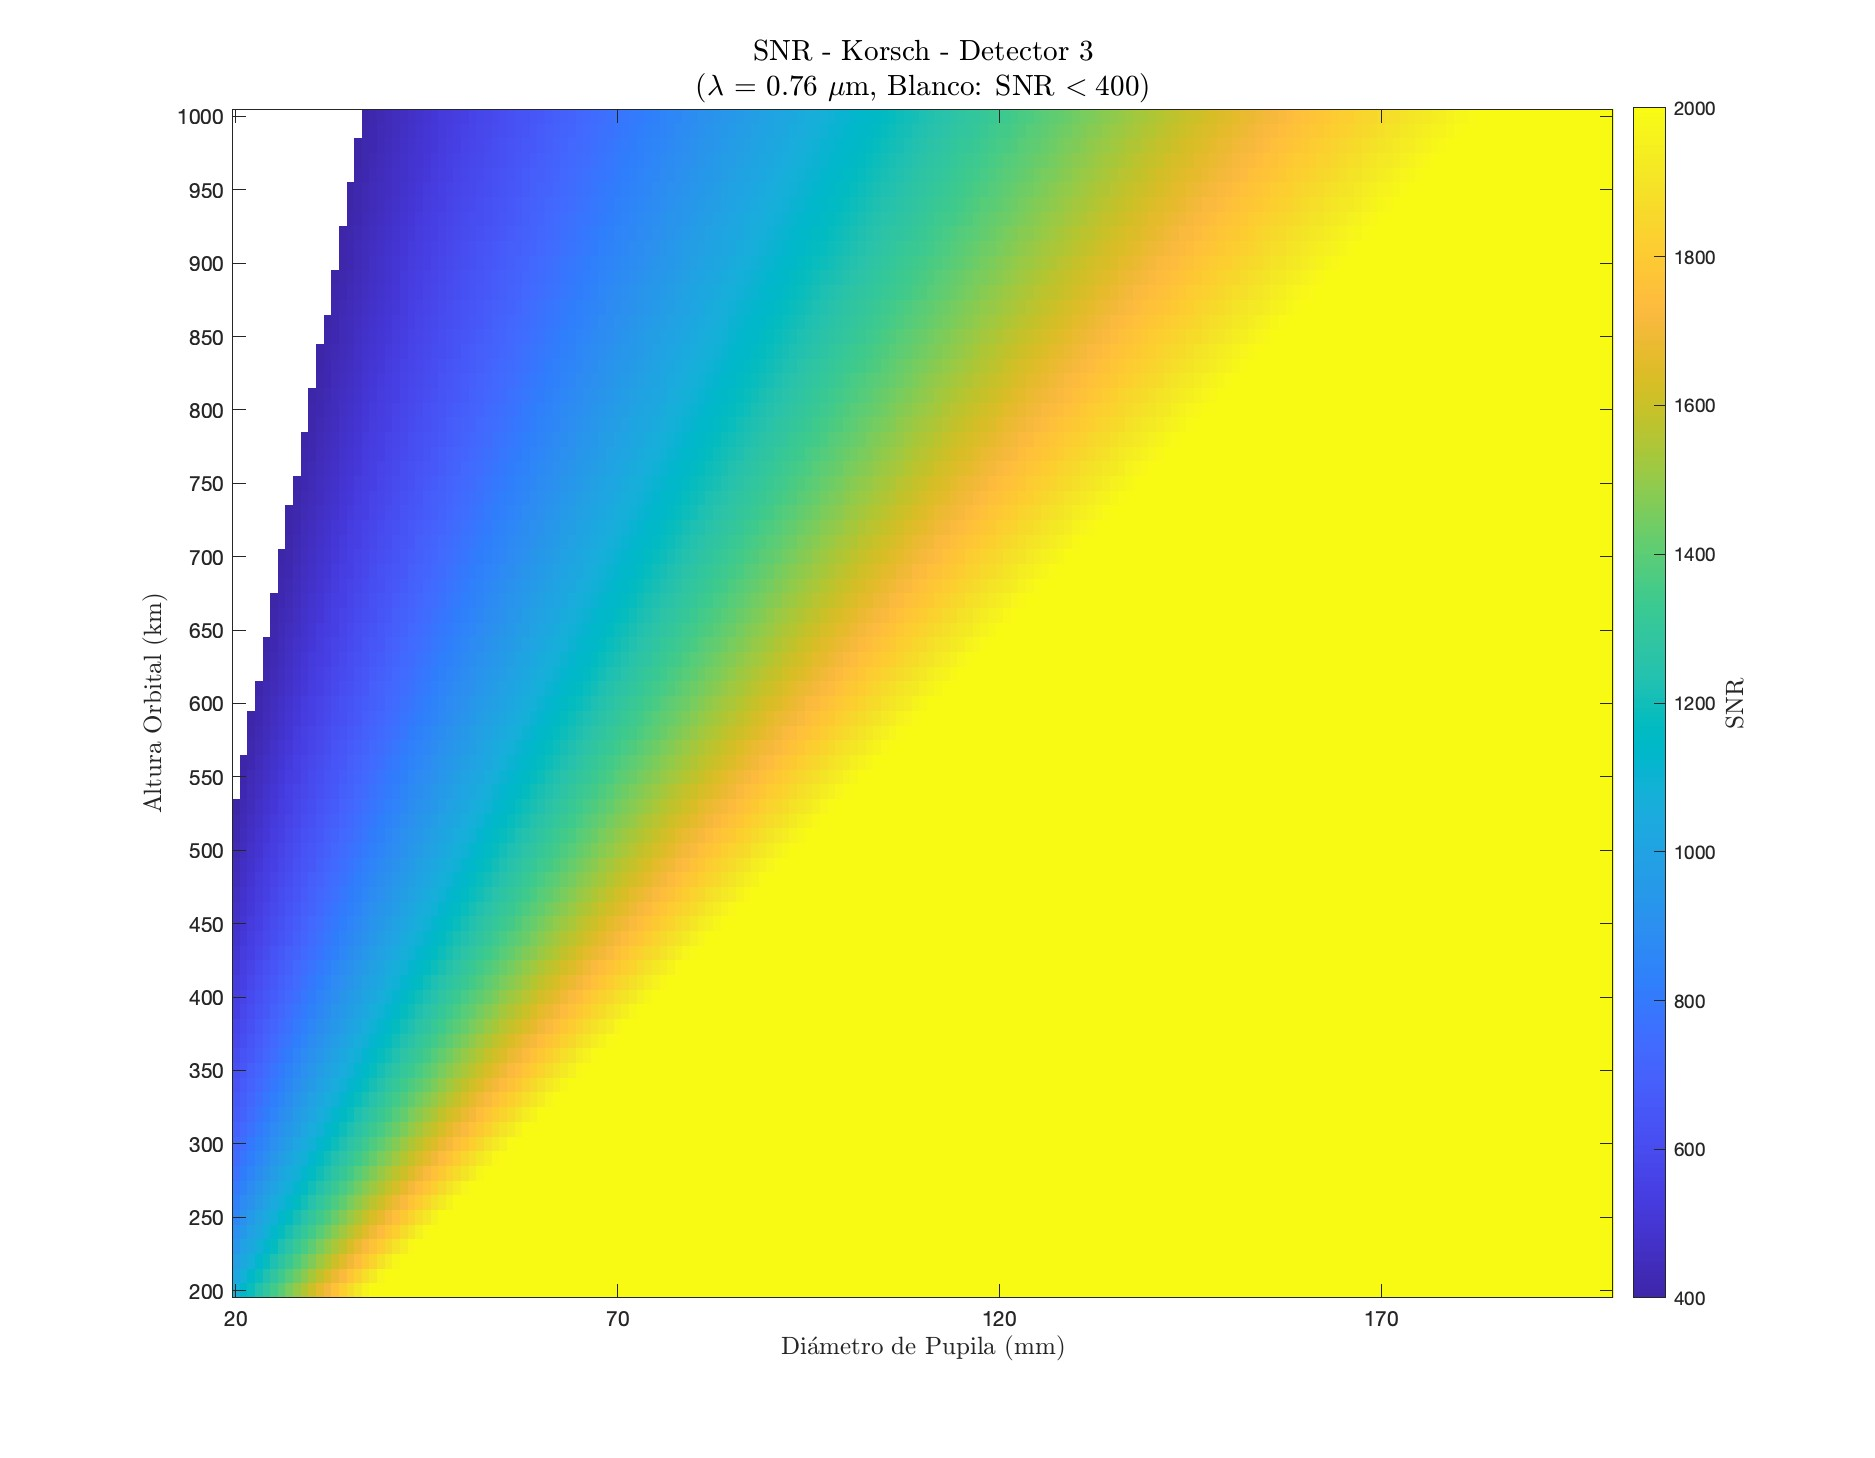
\includegraphics[width=0.48\linewidth]{4.Payload/SNR/SNR_Lambda3_Detector6_Telescopio2_heatmap.jpg} \\
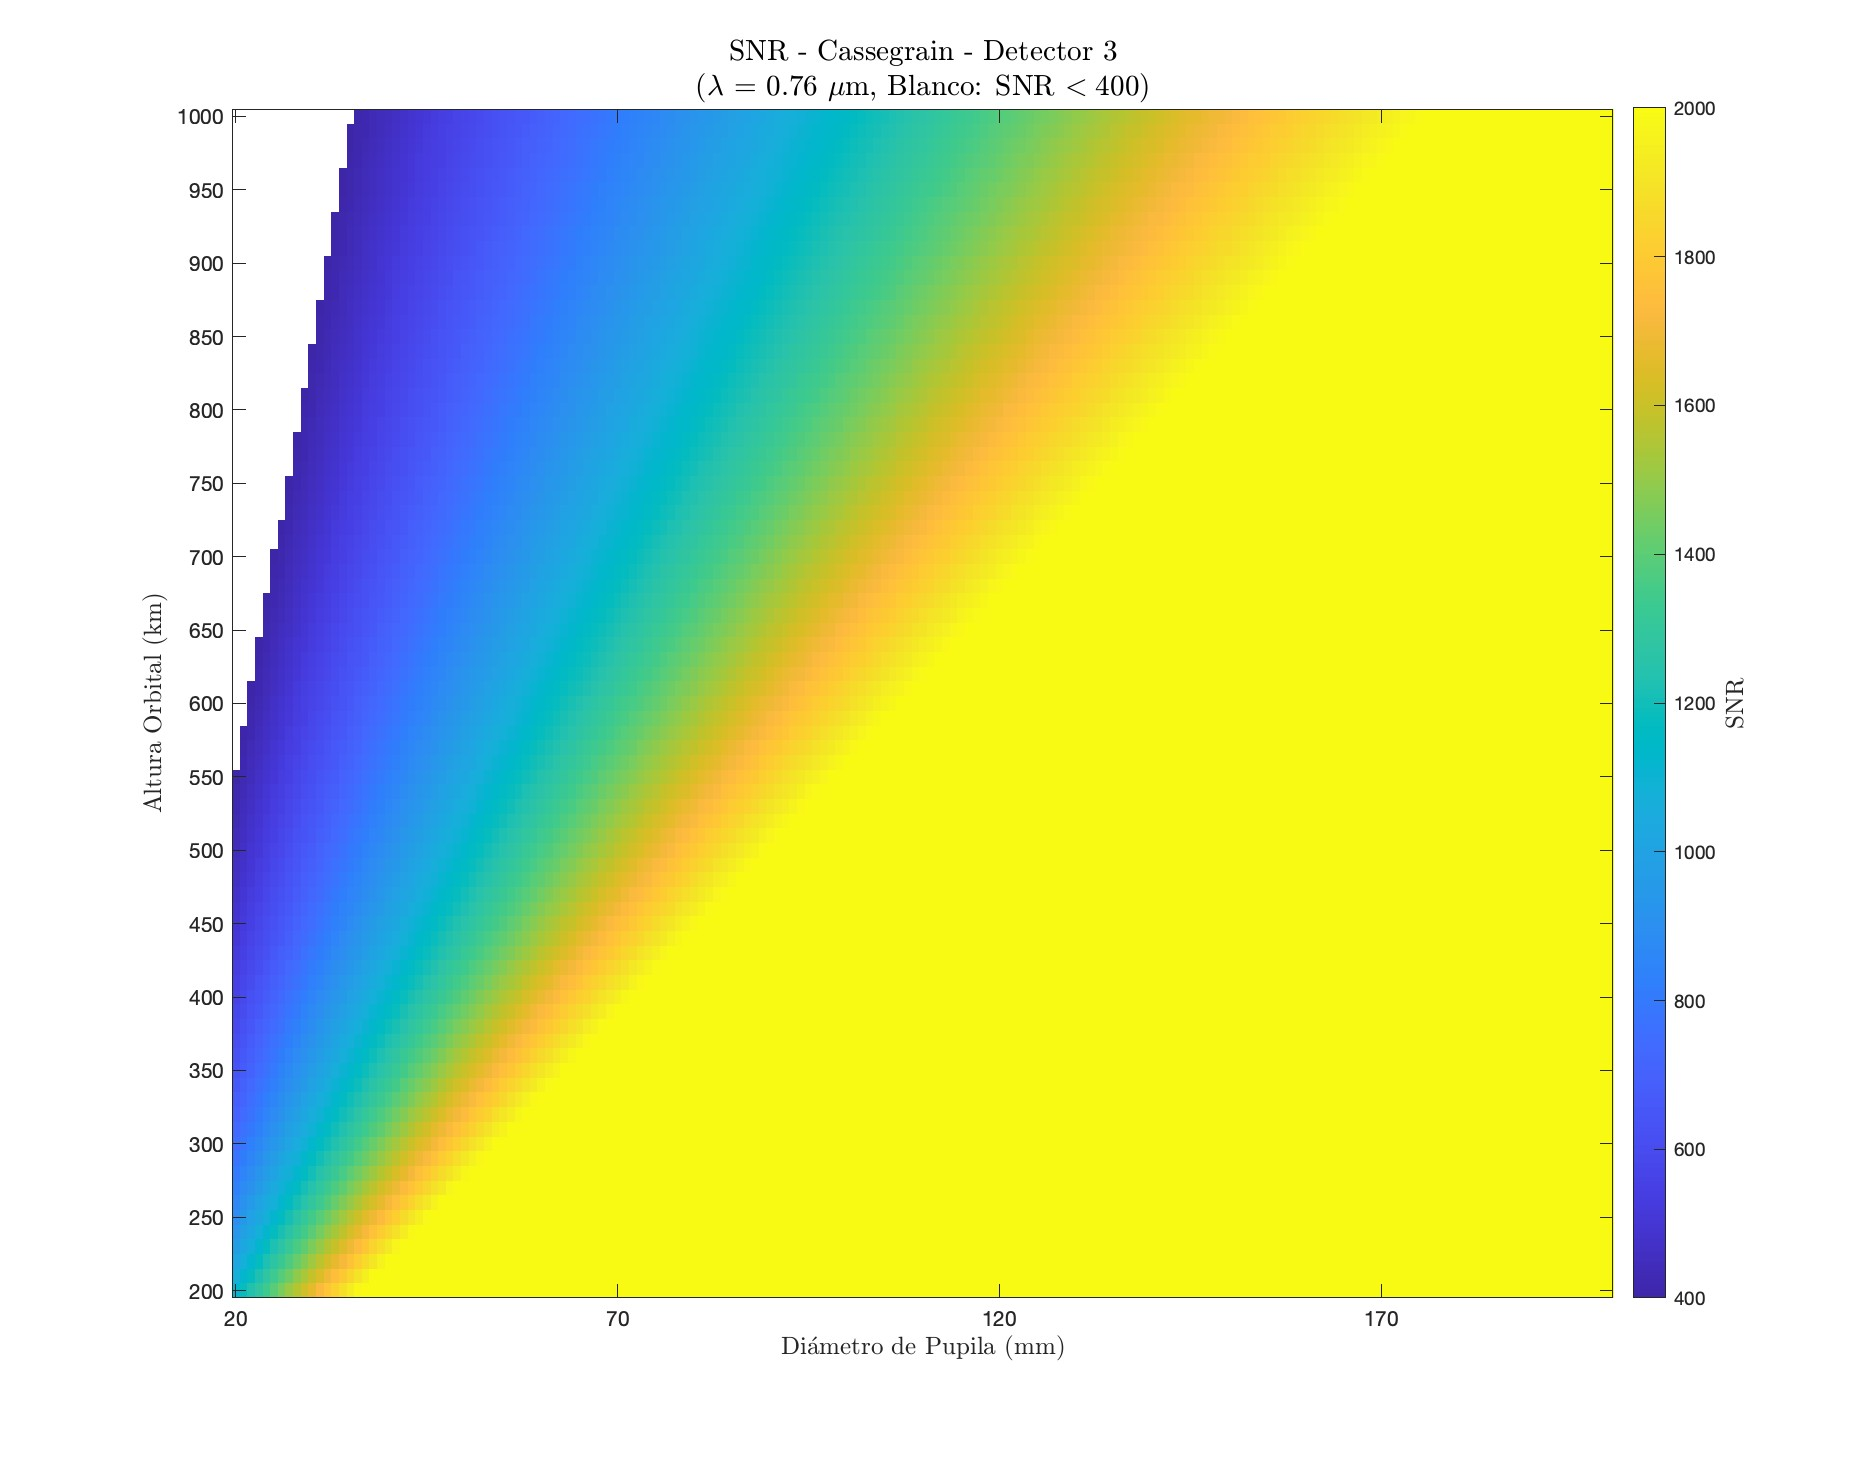
\includegraphics[width=0.48\linewidth]{4.Payload/SNR/SNR_Lambda3_Detector6_Telescopio3_heatmap.jpg} &
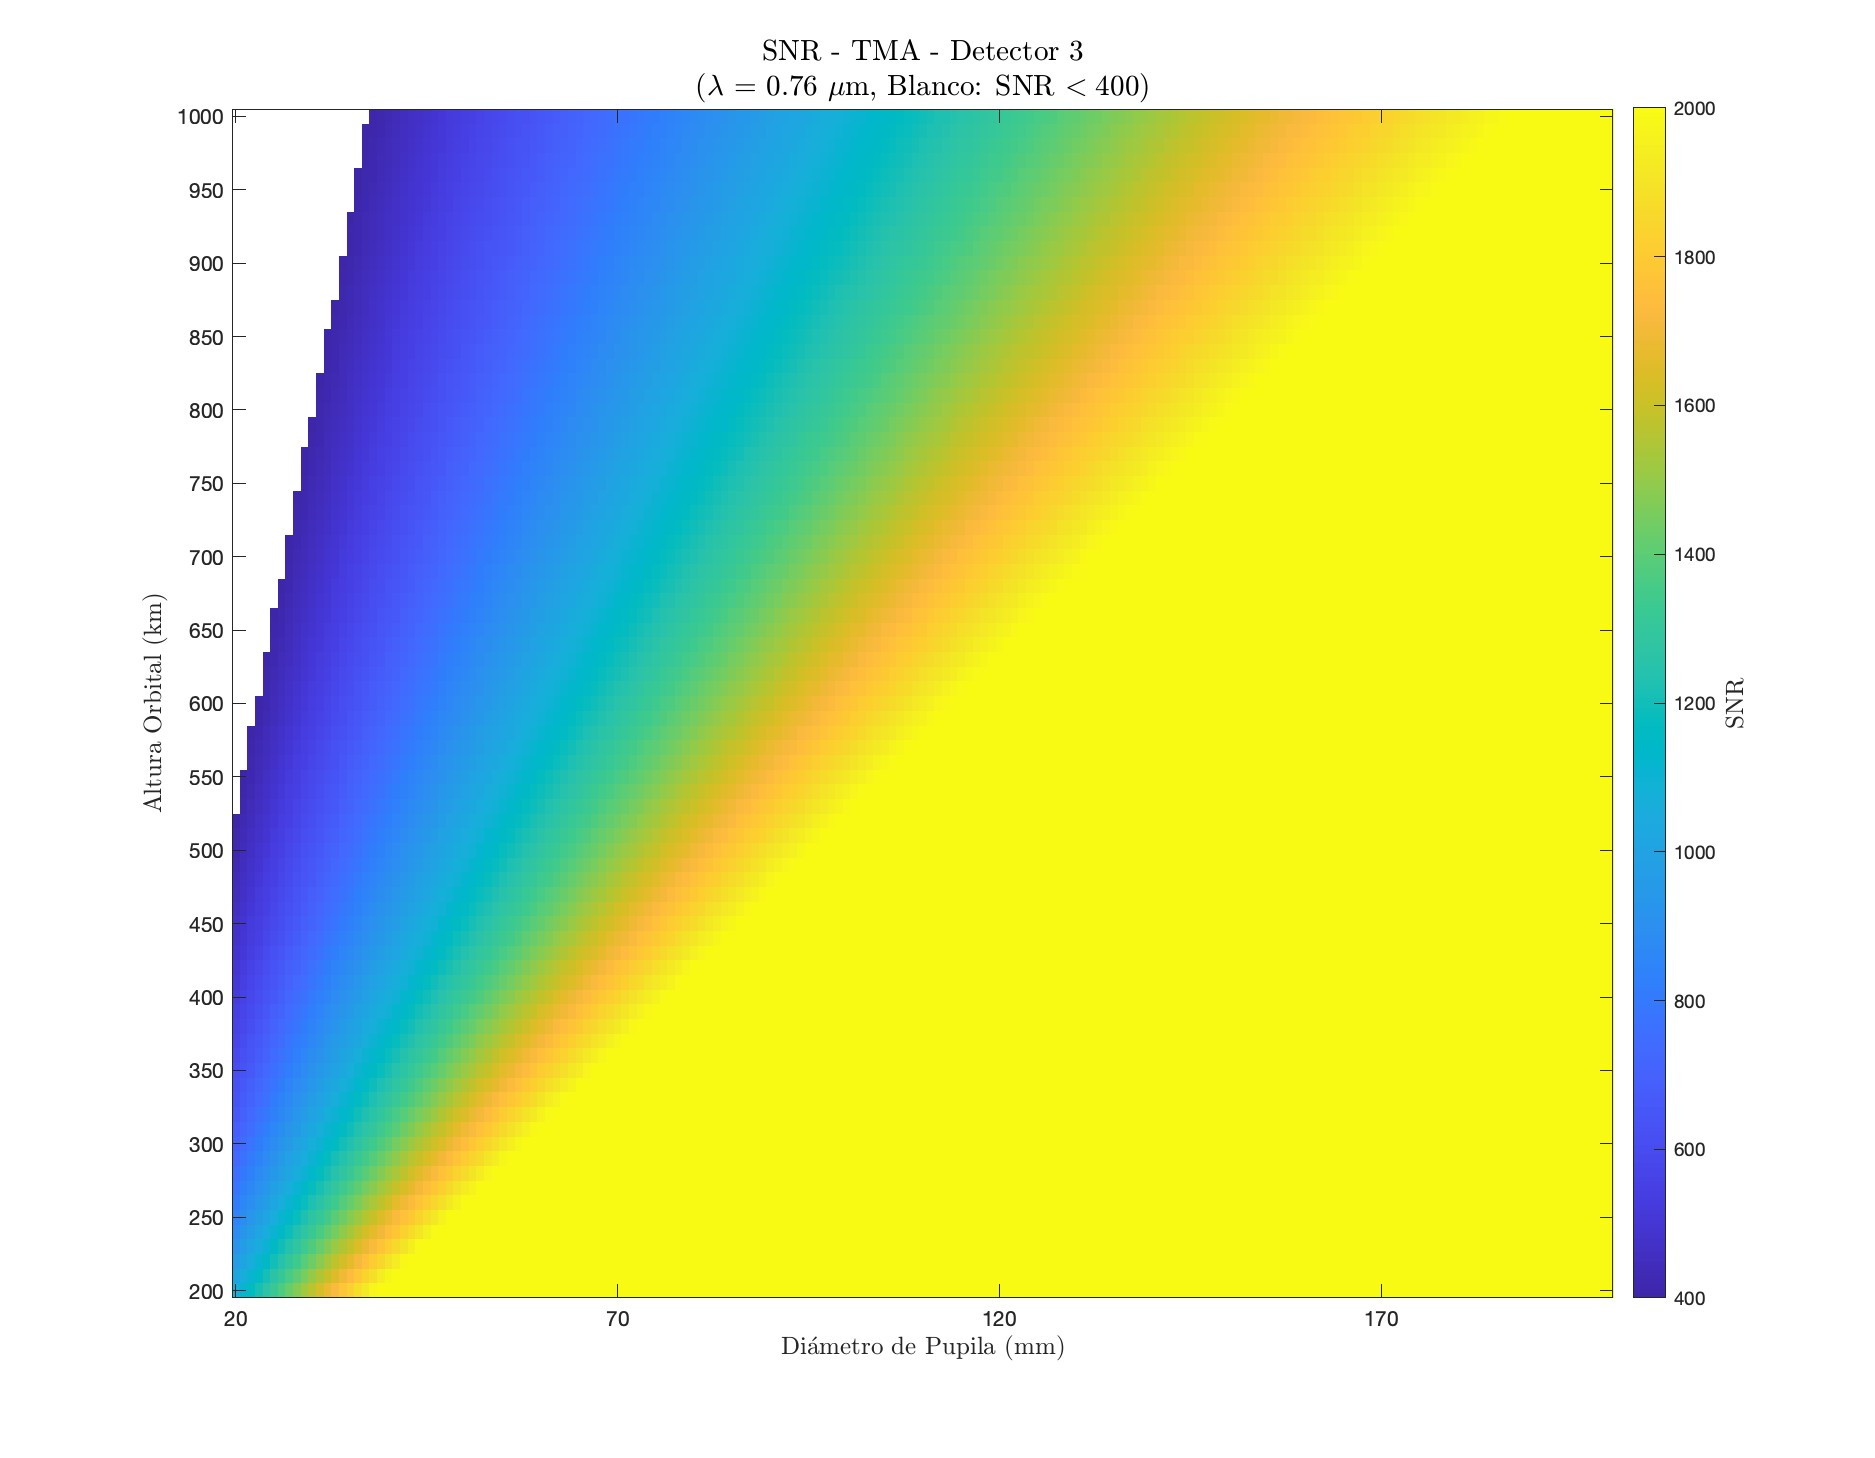
\includegraphics[width=0.48\linewidth]{4.Payload/SNR/SNR_Lambda3_Detector6_Telescopio4_heatmap.jpg} \\
\end{tabular}
\caption{Mapas de calor resultantes del calculo de SNR: Banda 0,76 \textmu m; Detector 3}
\end{figure}
\end{landscape}


De la interpretación de estos gráficos se obtienen las siguientes apreciaciones:

\begin{itemize}
    \item Este es, con diferencia, el requisito de misión menos restrictivo para el trabajo, pues, con los grandes tamaños de pixel y buenas eficiencias cuánticas del detector, junto con longitudes de onda mayores al visible, es sencillo conseguir altos valores de SNR.
    \item Se puede descartar la incorporación de TDI, ya que con una integración simple se captura una relación señal ruido que cumple holgadamente con el requisito de la misión para todos los casos. 
\end{itemize}

\section{Cobertura de la región de interés: Swath, FoV y tiempo de revisita}

Otro de los requerimientos impuestos por el cliente es el obtener un mapa cada 7 días en la región, o lo que es lo mismo, un tiempo de revisita de 7 días o menor. Si se comparan con otras misiones de observación similares, se puede observar que es un tiempo exigente que requiere habitualmente de una constelación por lo que será de los parámetros más limitantes a la hora de encontrar la solución óptima:

%% Ejemplos cobertura
\begin{table}[H]
\caption{Comparativa de tiempos de revisita de misiones satelitales.}
\centering
\begin{tabular}{@{}llll@{}}
\toprule
             & Nº Satélites & \textit{Swath} (km) & Tiempo revisita\tablefootnote{Estos valores son más favorables que los calculados en este trabajo, pues no se consideran los factores limitantes descritos en esta página. Por ello, no serán directamente comparables a los resultados obtenidos, aunque permite hacerse una idea aproximada de la solución} (días) \\ \midrule
Landsat 8 \cite{li2020global}   & 1                & 185                 & 16                     \\
Landsat Next \cite{copernicus2025sentinel} & 3                & 164                 & 6                      \\
Sentinel-2  \cite{neigh2023landsat} & 2                & 290                 & 5                      \\ \bottomrule
\end{tabular}

\label{tab:revisitlandsat}
\end{table}


Además, se tendrán en cuenta 2 factores adicionales para el cálculo:
\begin{itemize}
    \item \textbf{Solapamiento del swath}: Para asegurar la cobertura completa de la región entre pasadas, se establece un \textbf{factor de solapamiento del swath mínimo del 5\%} que compensa posibles desviaciones en la proyección del swath y pérdidas de altura del satélite antes de la reinyección orbital.
    \item \textbf{Cobertura de nubes}: A diferencia de otros sistemas de observación, como el SAR (Radar de Apertura Sintética, o \textit{Synthetic Aperture Radar}, \cite{lou2020sar}), los detectores SWIR pasivos no son capaces de capturar la señal de la superficie terrestre a través de los cúmulos nubosos. Según el enunciado impuesto, \say{\textit{la cobertura de nubes sobre EE. UU. es un día cubierto por cada cinco descubiertos}}, por lo que se considera un \textbf{factor de 1/6 de pasadas del satélite no efectivas}.
\end{itemize}

\begin{figure}[H]
    \centering
    \begin{subfigure}[t]{0.45\textwidth}
        \centering
        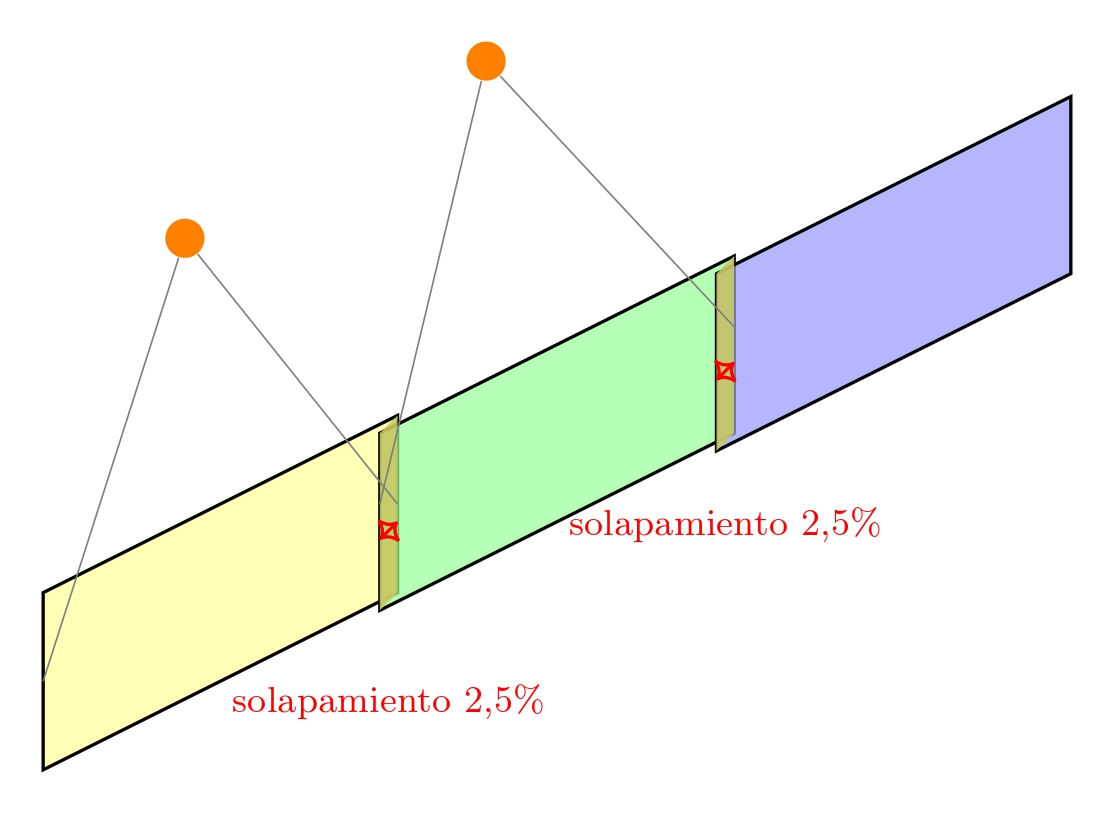
\includegraphics[width=\linewidth]{4.Payload/TFG_Tikz-1.jpg}
        \caption{Solapamiento del swath. \\ Fuente: Elaboración propia}
        \label{fig:img3}
    \end{subfigure}
    \hspace{0.05\textwidth}
    \begin{subfigure}[t]{0.45\textwidth}
        \centering
        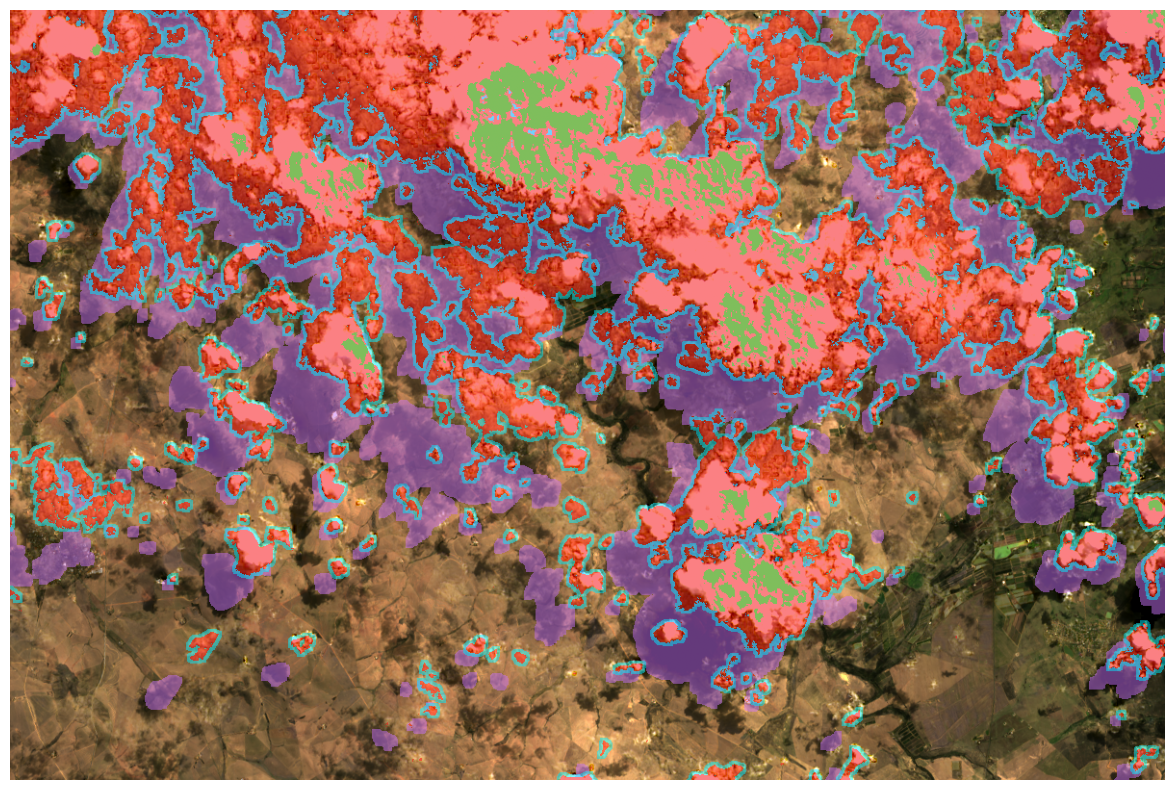
\includegraphics[width=\linewidth]{4.Payload/cloudcov.png}
        \caption{Datos no válidos debido a cobertura de nubes de la misión Landsat, en rojo. \\ Fuente: \cite{osullivan2023removing}}
        \label{fig:img4}
    \end{subfigure}
    \caption{Factores de limitación del swath en el problema de la cobertura}
\end{figure}


Para realizar la computación de la cobertura en la región de interés, se va a utilizar un software \textit{open-source} desarrollado en el paper \textit{A Semi-Analytical Method for Calculating Revisit Time for Satellite Constellations with Discontinuous Coverage} \cite{crisp2018semi}. Para aplicar dicho código al presente trabajo, se ha desarrollado un \textit{wrapper}, es decir, una función que actúa como interfaz de adaptación entre los parámetros específicos del presente estudio y las funciones originales del software mencionado. Con ello, se pueden extraer mapas de calor que expongan, en función de la altura orbital y el \textit{swath}\footnote{Discretizados ambos en pasos de 10 km}, los tiempos de revisita necesarios para la región de interés. Evaluaremos distintas configuraciones:

\begin{itemize}
    \item Configuración (i): 1 único satélite con 1 telescopio embarcado.
    \item Config. (ii): 1 satélite con 2 telescopios embarcados. Los telescopios serán dispuestos según la Figura \ref{fig:img1}, esencialmente duplicando el FoV límite.
    \item Config. (iii): Constelación de 2 satélites ($i:2/1/0$\footnote{Escrito en notación de Walker \cite{walker1991phase}}).
    \item Config. (iv): Constelación de 2 satélites, con 2 telescopios embarcados en cada uno. ($i:2/1/0$).
    \item Config. (v): Constelación de 3 satélites ($i:3/1/0$).
\end{itemize}

En todas las constelaciones, los satélites se dispondrán desfasados en anomalía verdadera de manera que $\Delta \nu = 360º/n $ siendo $n =$ Nº satélites, dentro de la misma órbita (véase Figura \ref{fig:img2}). Esto permite reducir en un factor de $n$ la distancia entre pasadas a medida que rota la Tierra, consiguiendo tiempos de revisita menores, manteniendo así para todos los satélites el mismo valor de LTAN.

\begin{figure}[H]
    \centering
    \begin{subfigure}[t]{0.45\textwidth}
        \centering
        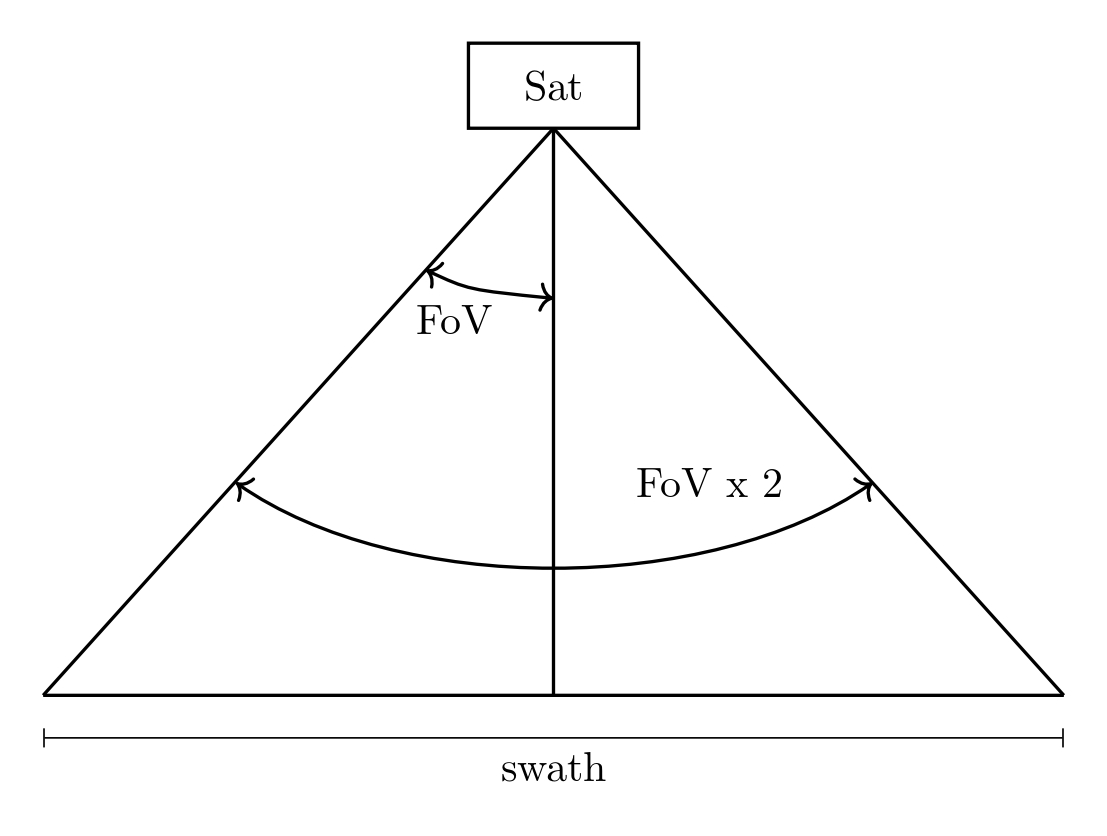
\includegraphics[width=\linewidth]{4.Payload/TFG_Tikz-2.jpg}
        \caption{Disposición de dos telescopios embarcados en un satélite. \\ Fuente: Elaboración propia}
        \label{fig:img1}
    \end{subfigure}
    \hspace{0.05\textwidth}
    \begin{subfigure}[t]{0.45\textwidth}
        \centering
        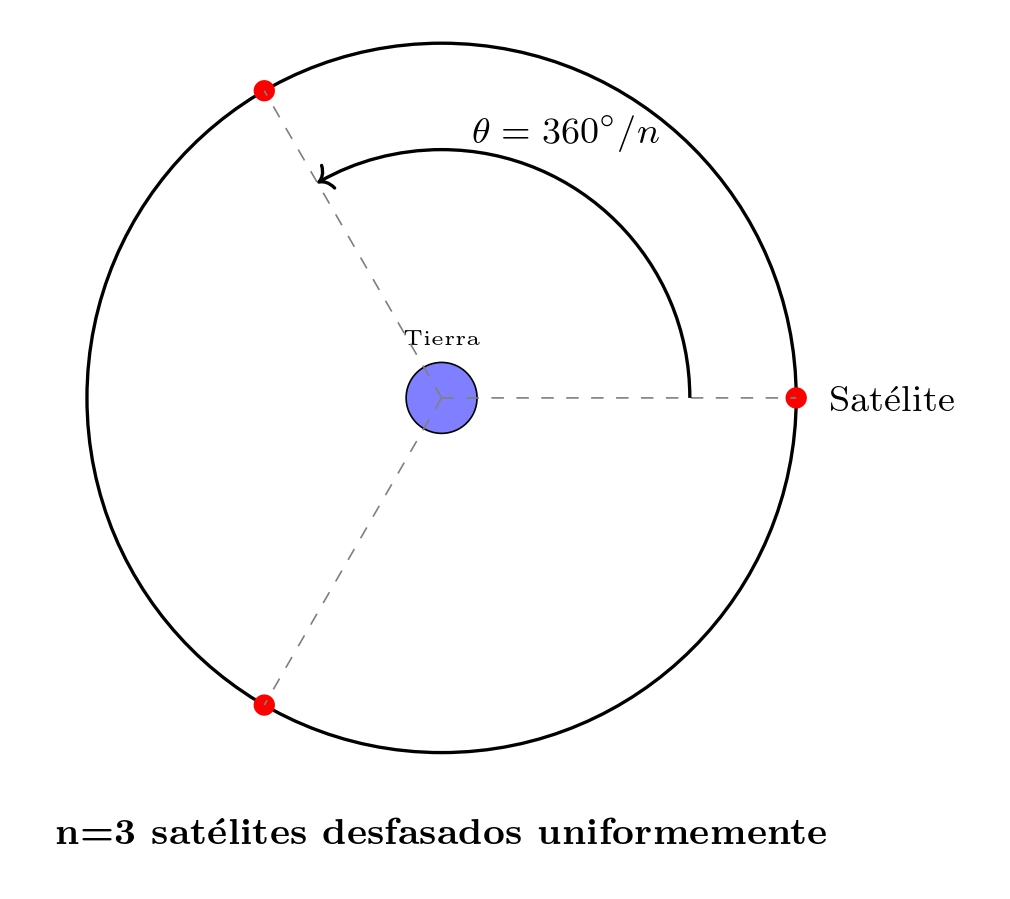
\includegraphics[width=\linewidth]{4.Payload/TFG_Tikz-3.jpg}
        \caption{Desfase de la constelación de satélites en anomalía verdadera. \\ Fuente: Elaboración propia.}
        \label{fig:img2}
    \end{subfigure}
    \caption{Esquemas de las configuraciones evaluadas en el problema de la cobertura.}
    \label{fig:configs}
\end{figure}

Se consideran dos limitaciones al \textit{swath}:
\begin{itemize}
    \item El FoV de cada telescopio, definido en la tabla \ref{tab:tabla_telescopios}, que limita el swath en función de la altura, mediante la relación \ref{fov}
    \item El array del detector, mediante la ecuación \ref{swath}. Para ampliarlo y dar más flexibilidad a esta restricción, se considera el uso de hasta 3 detectores en linea.
\end{itemize}

Además, solo se considerará el territorio EE. UU. continental, con una \textbf{latitud inferior límite de 25º N}. Ya que el interés del cliente reside en el mapeo de las principales ciudades, se pueden excluir, por simplicidad de cálculo, otros territorios del país como Hawaii, Puerto Rico y otros territorios de ultramar. Con ello, se procede a realizar la computación y exponer los resultados en las siguientes páginas:

%% Graficas 2 SAT 2TEL
\begin{landscape}
\begin{figure}[p]
\centering
\vspace*{0.3cm}
\setlength{\tabcolsep}{4pt}
\renewcommand{\arraystretch}{0}
\begin{tabular}{cc}
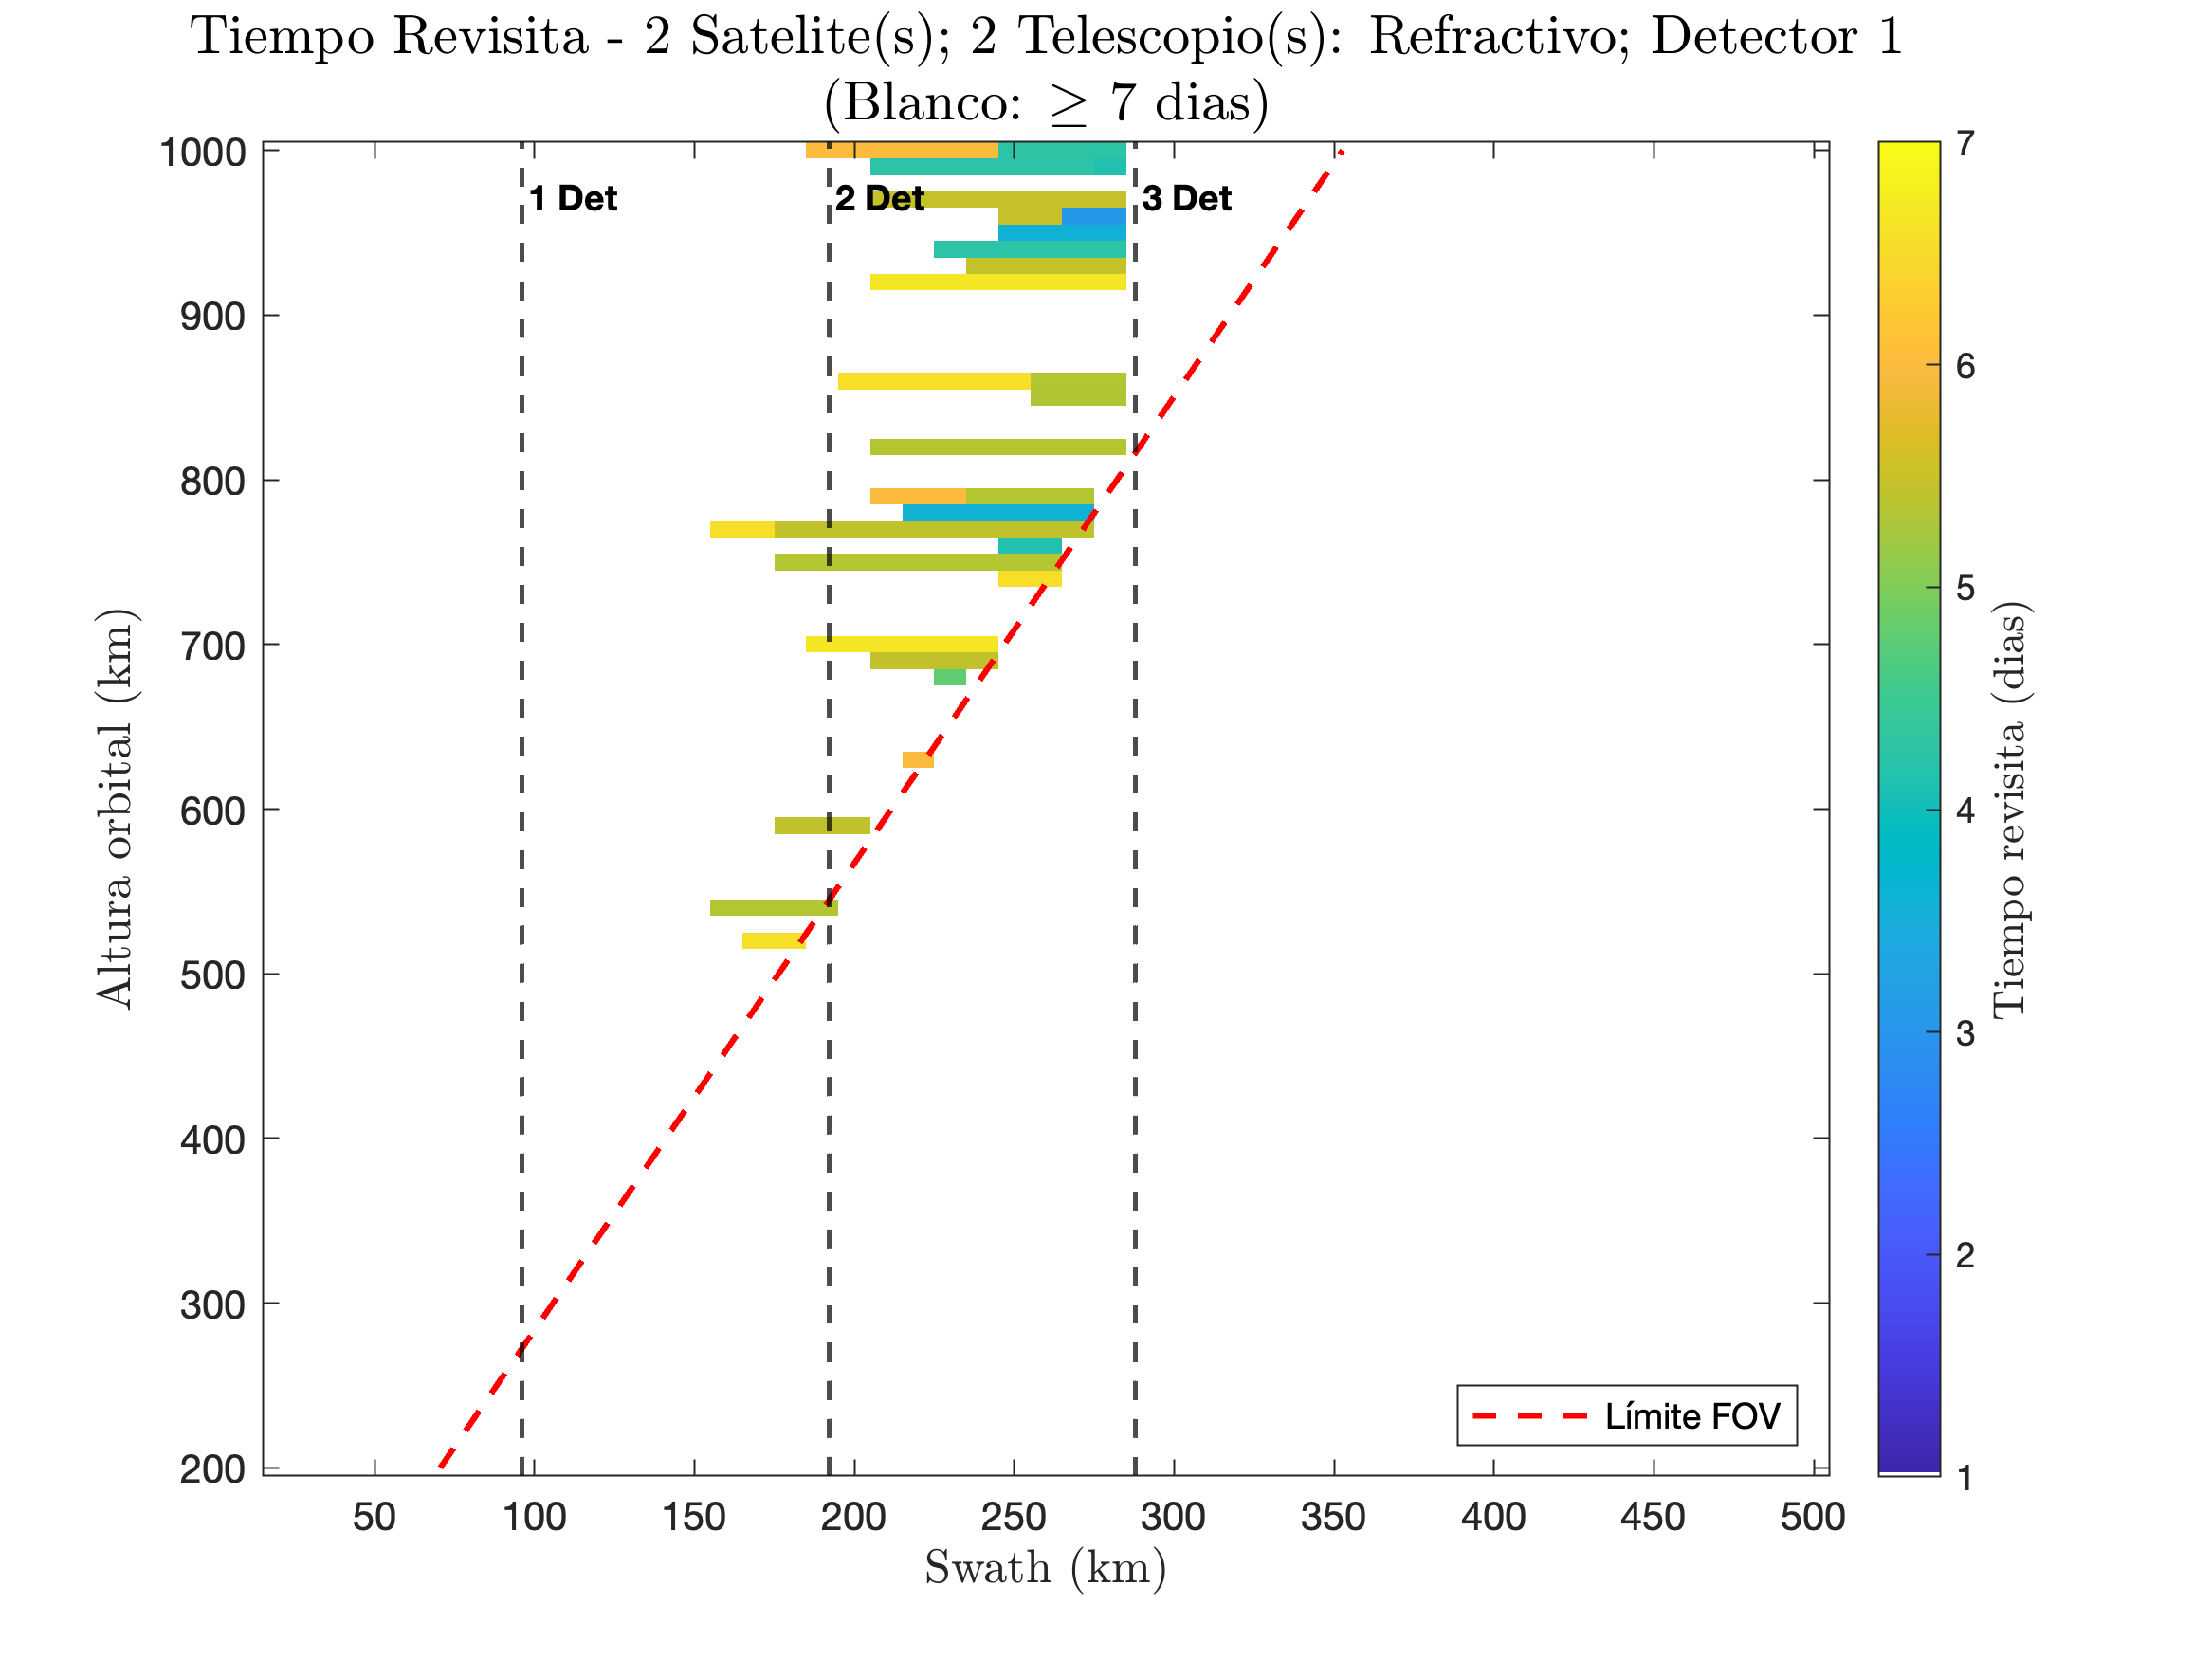
\includegraphics[width=0.48\linewidth]{4.Payload/Coverage/heatmap_2 Satelite(s); 2 Telescopio(s): Refractivo; Detector 1.jpg} &
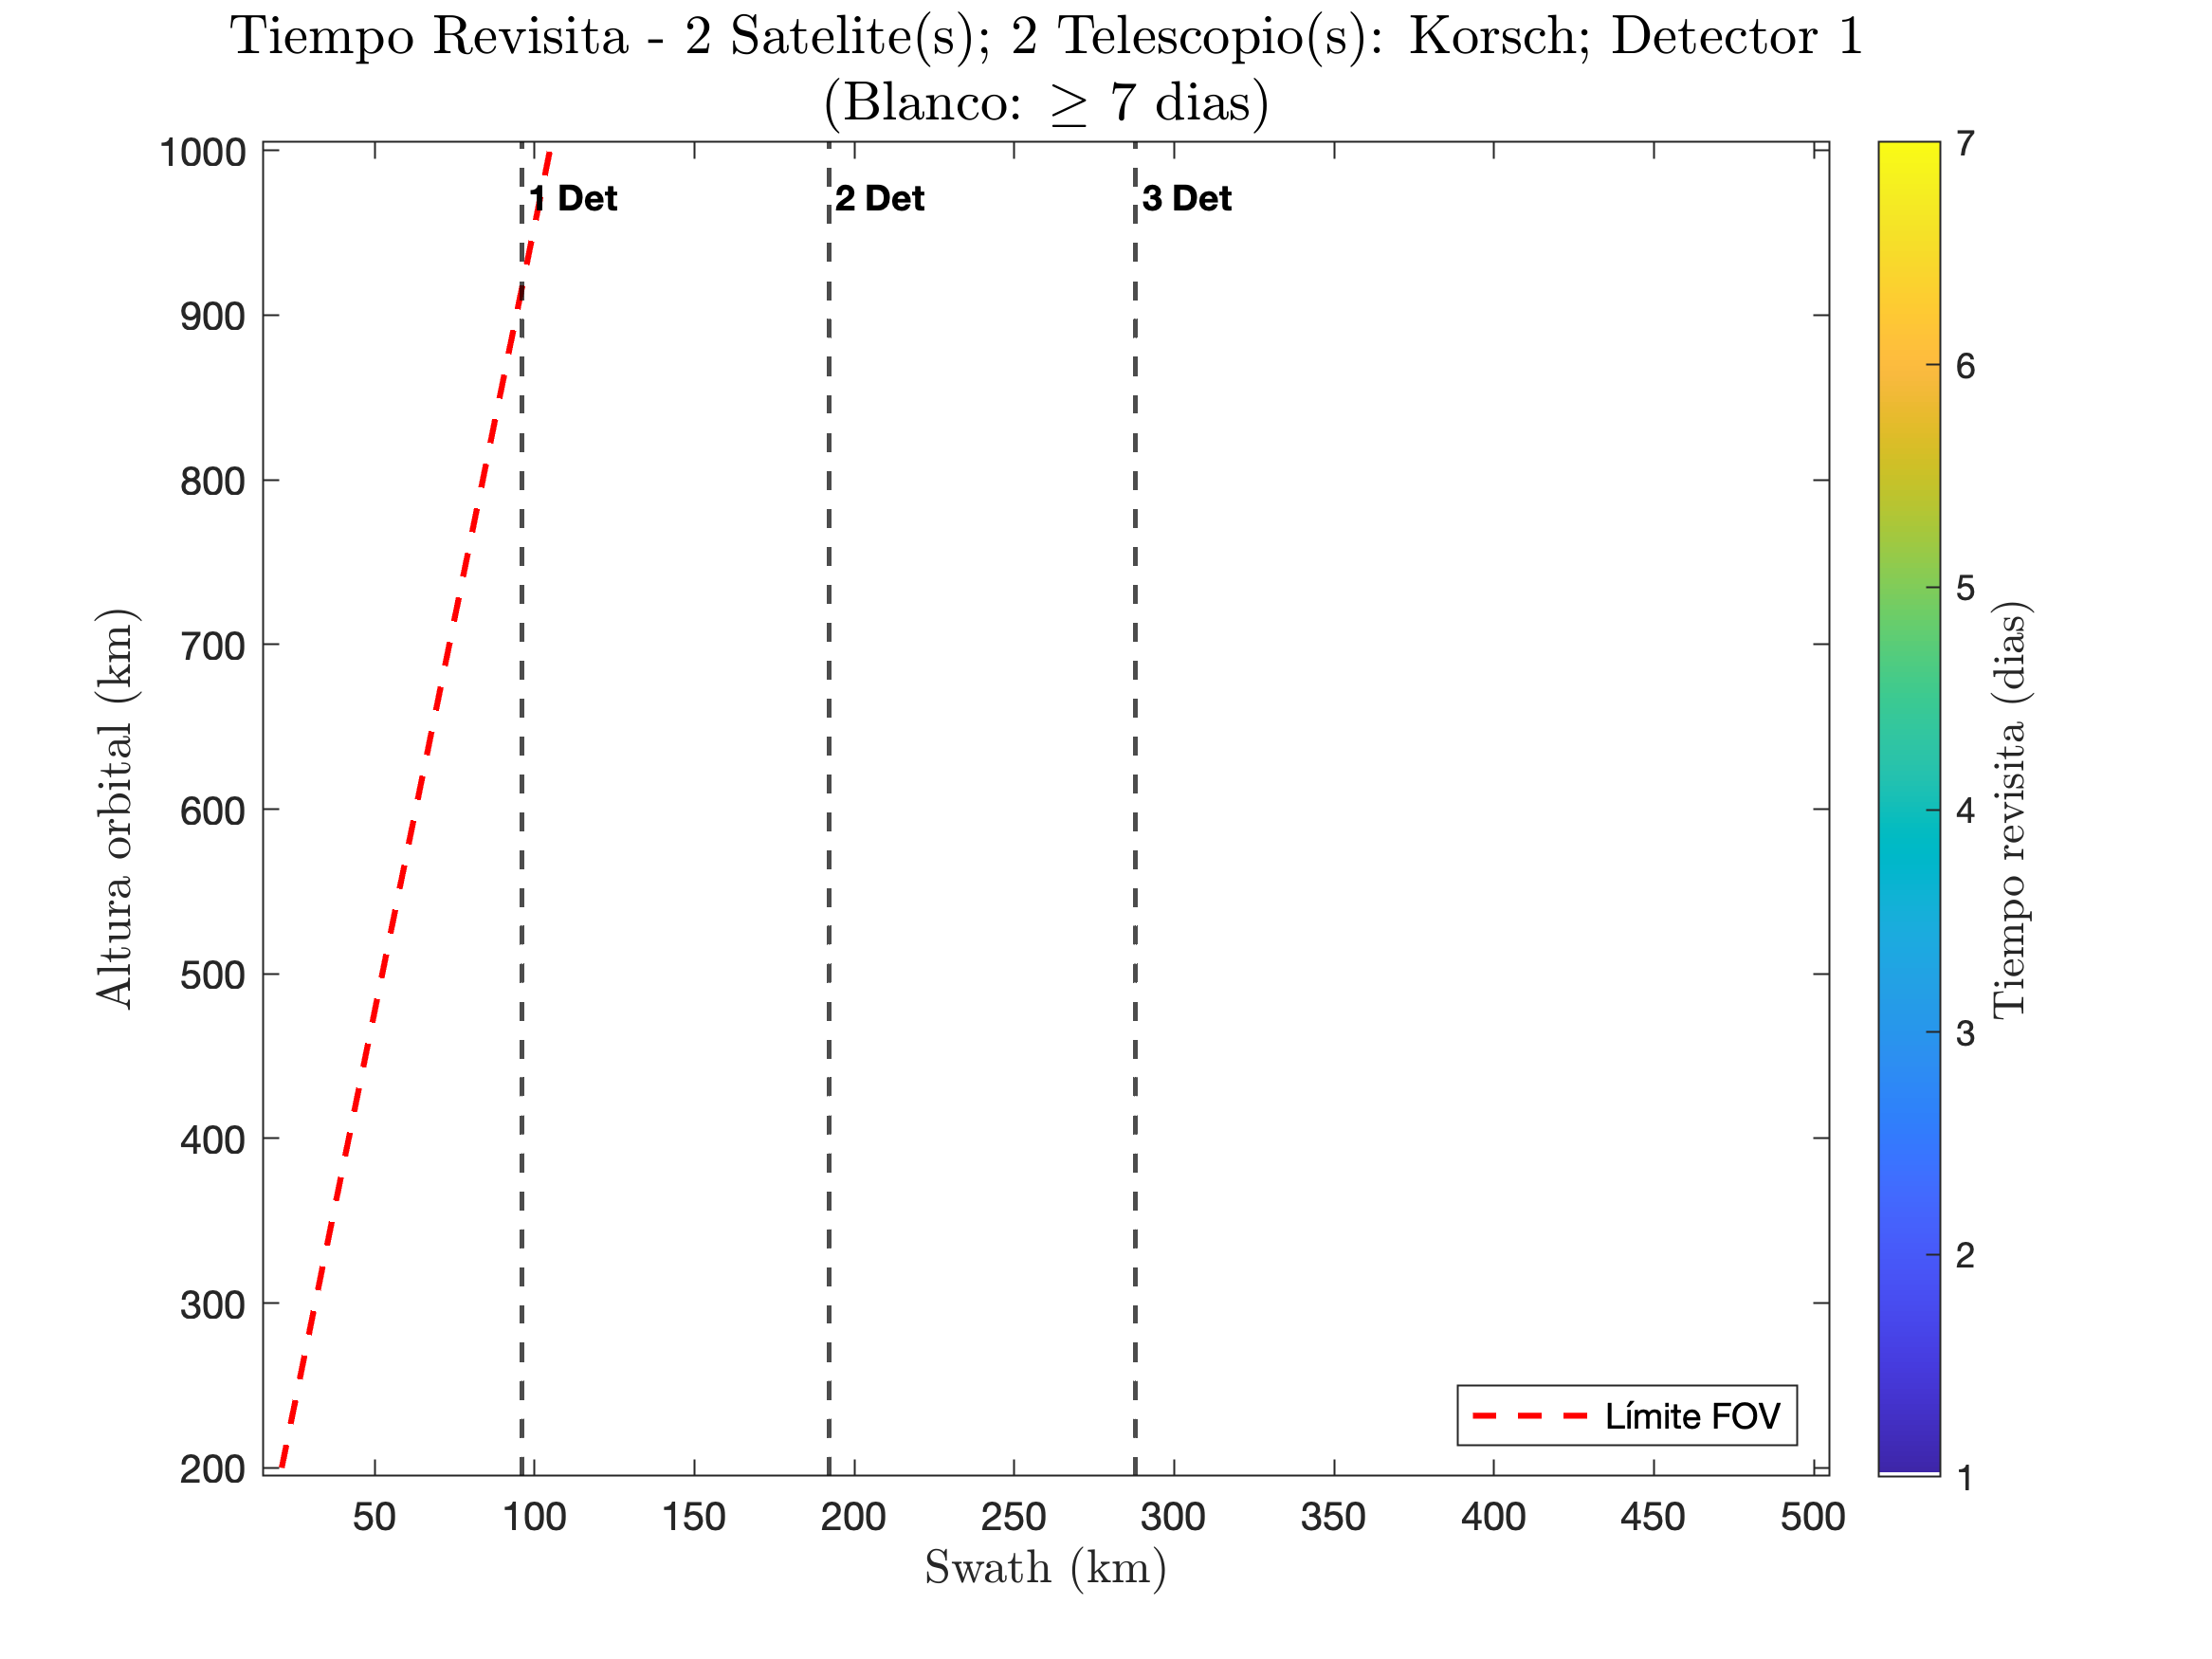
\includegraphics[width=0.48\linewidth]{4.Payload/Coverage/heatmap_2 Satelite(s); 2 Telescopio(s): Korsch; Detector 1.jpg} \\
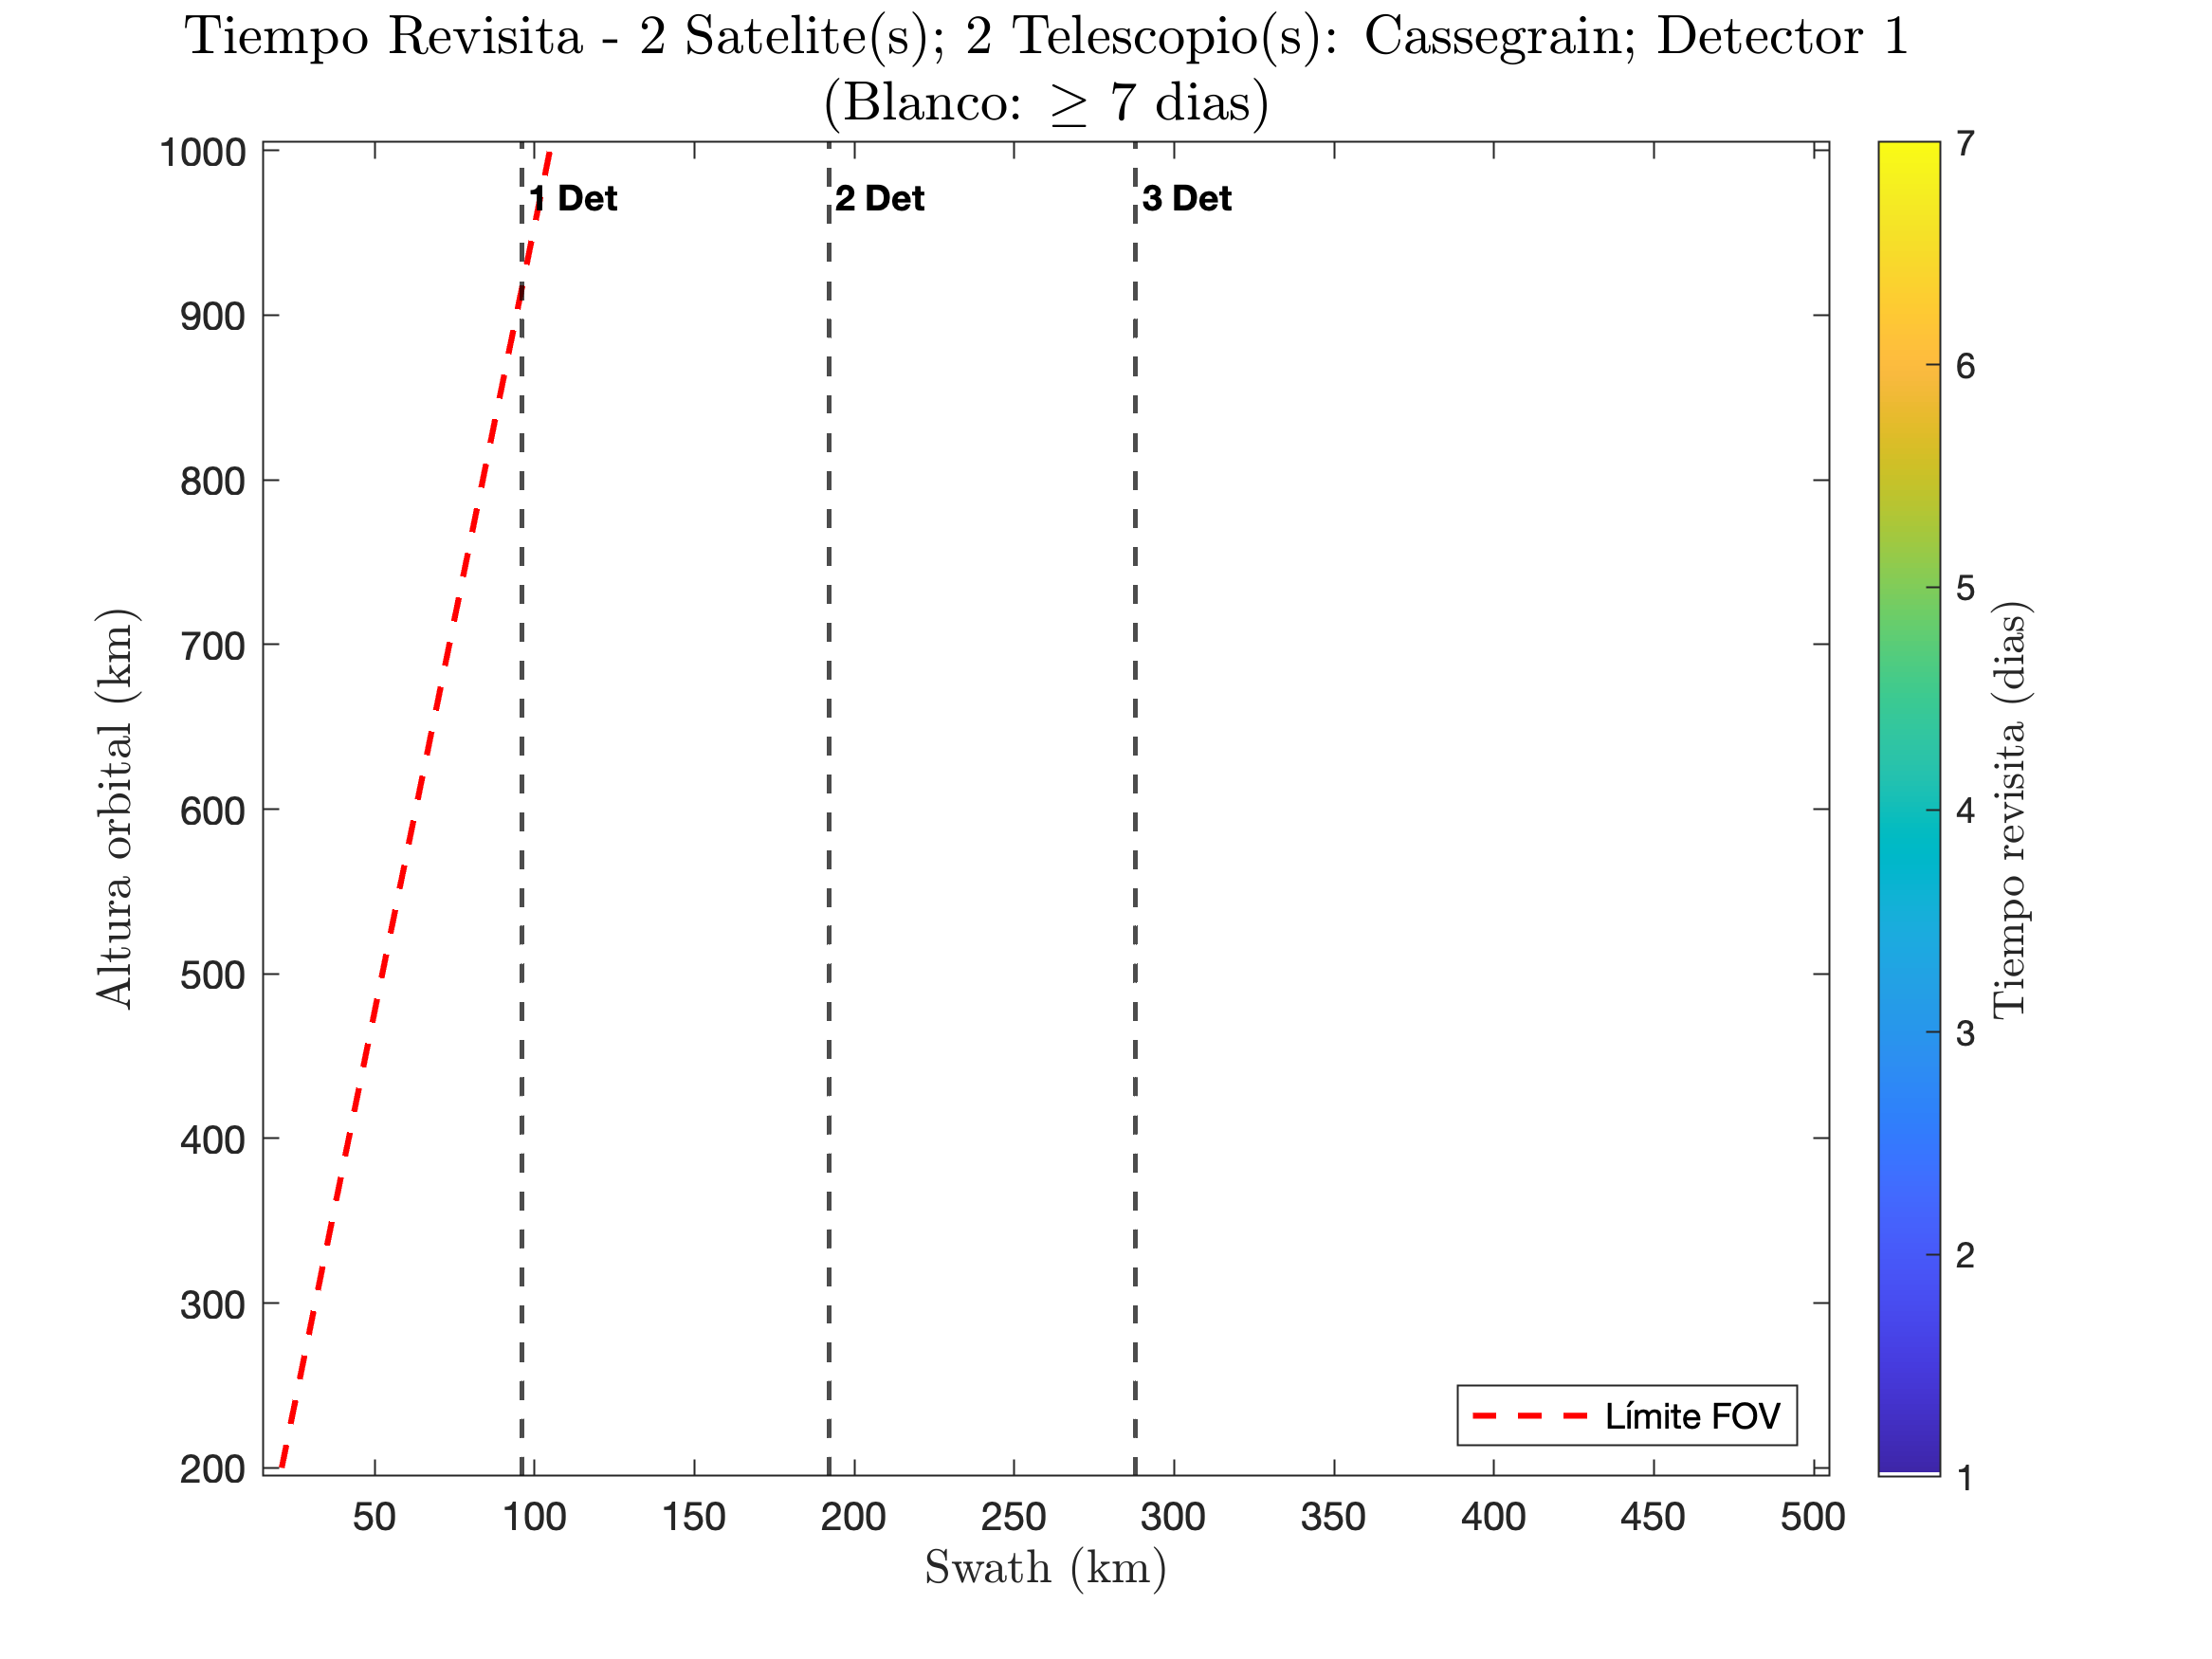
\includegraphics[width=0.48\linewidth]{4.Payload/Coverage/heatmap_2 Satelite(s); 2 Telescopio(s): Cassegrain; Detector 1.jpg} &
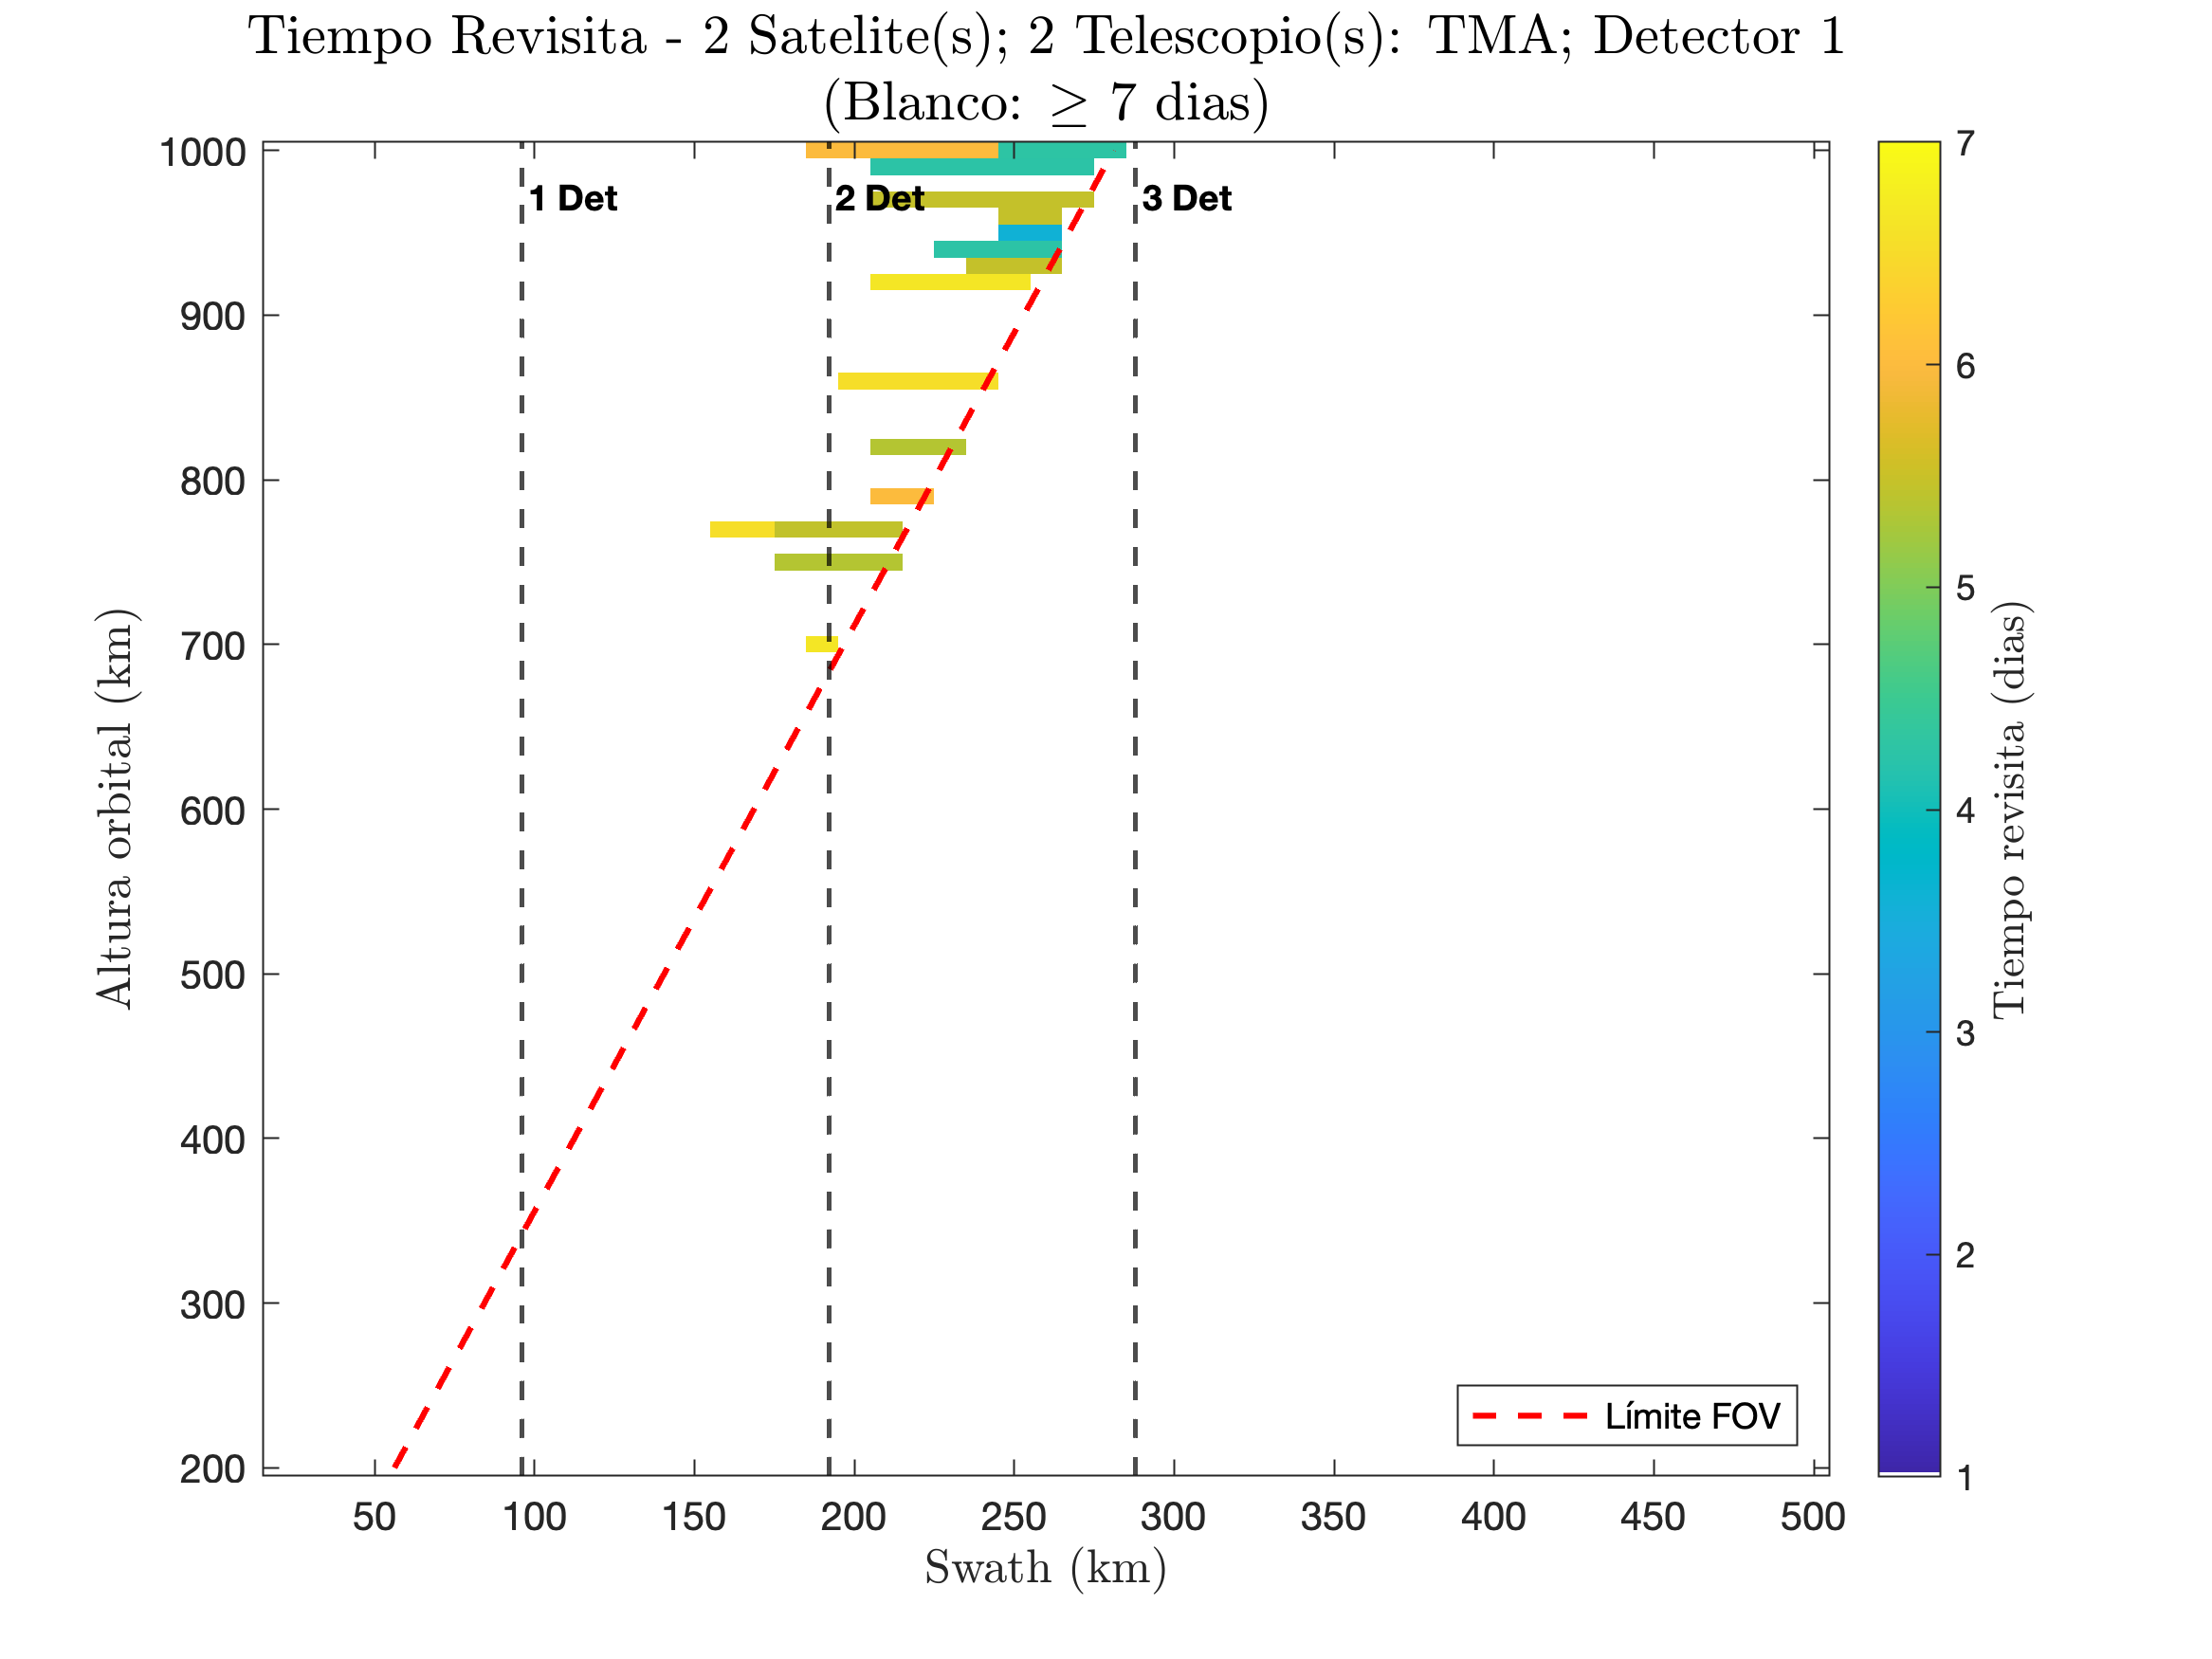
\includegraphics[width=0.48\linewidth]{4.Payload/Coverage/heatmap_2 Satelite(s); 2 Telescopio(s): TMA; Detector 1.jpg} \\
\end{tabular}
\caption{Mapas de calor resultantes del cálculo de cobertura para el Detector 1, con 2 satélites y 2 telescopios.}
\end{figure}
\end{landscape}

\begin{landscape}
\begin{figure}[p]
\centering
\vspace*{0.3cm}
\setlength{\tabcolsep}{4pt}
\renewcommand{\arraystretch}{0}
\begin{tabular}{cc}
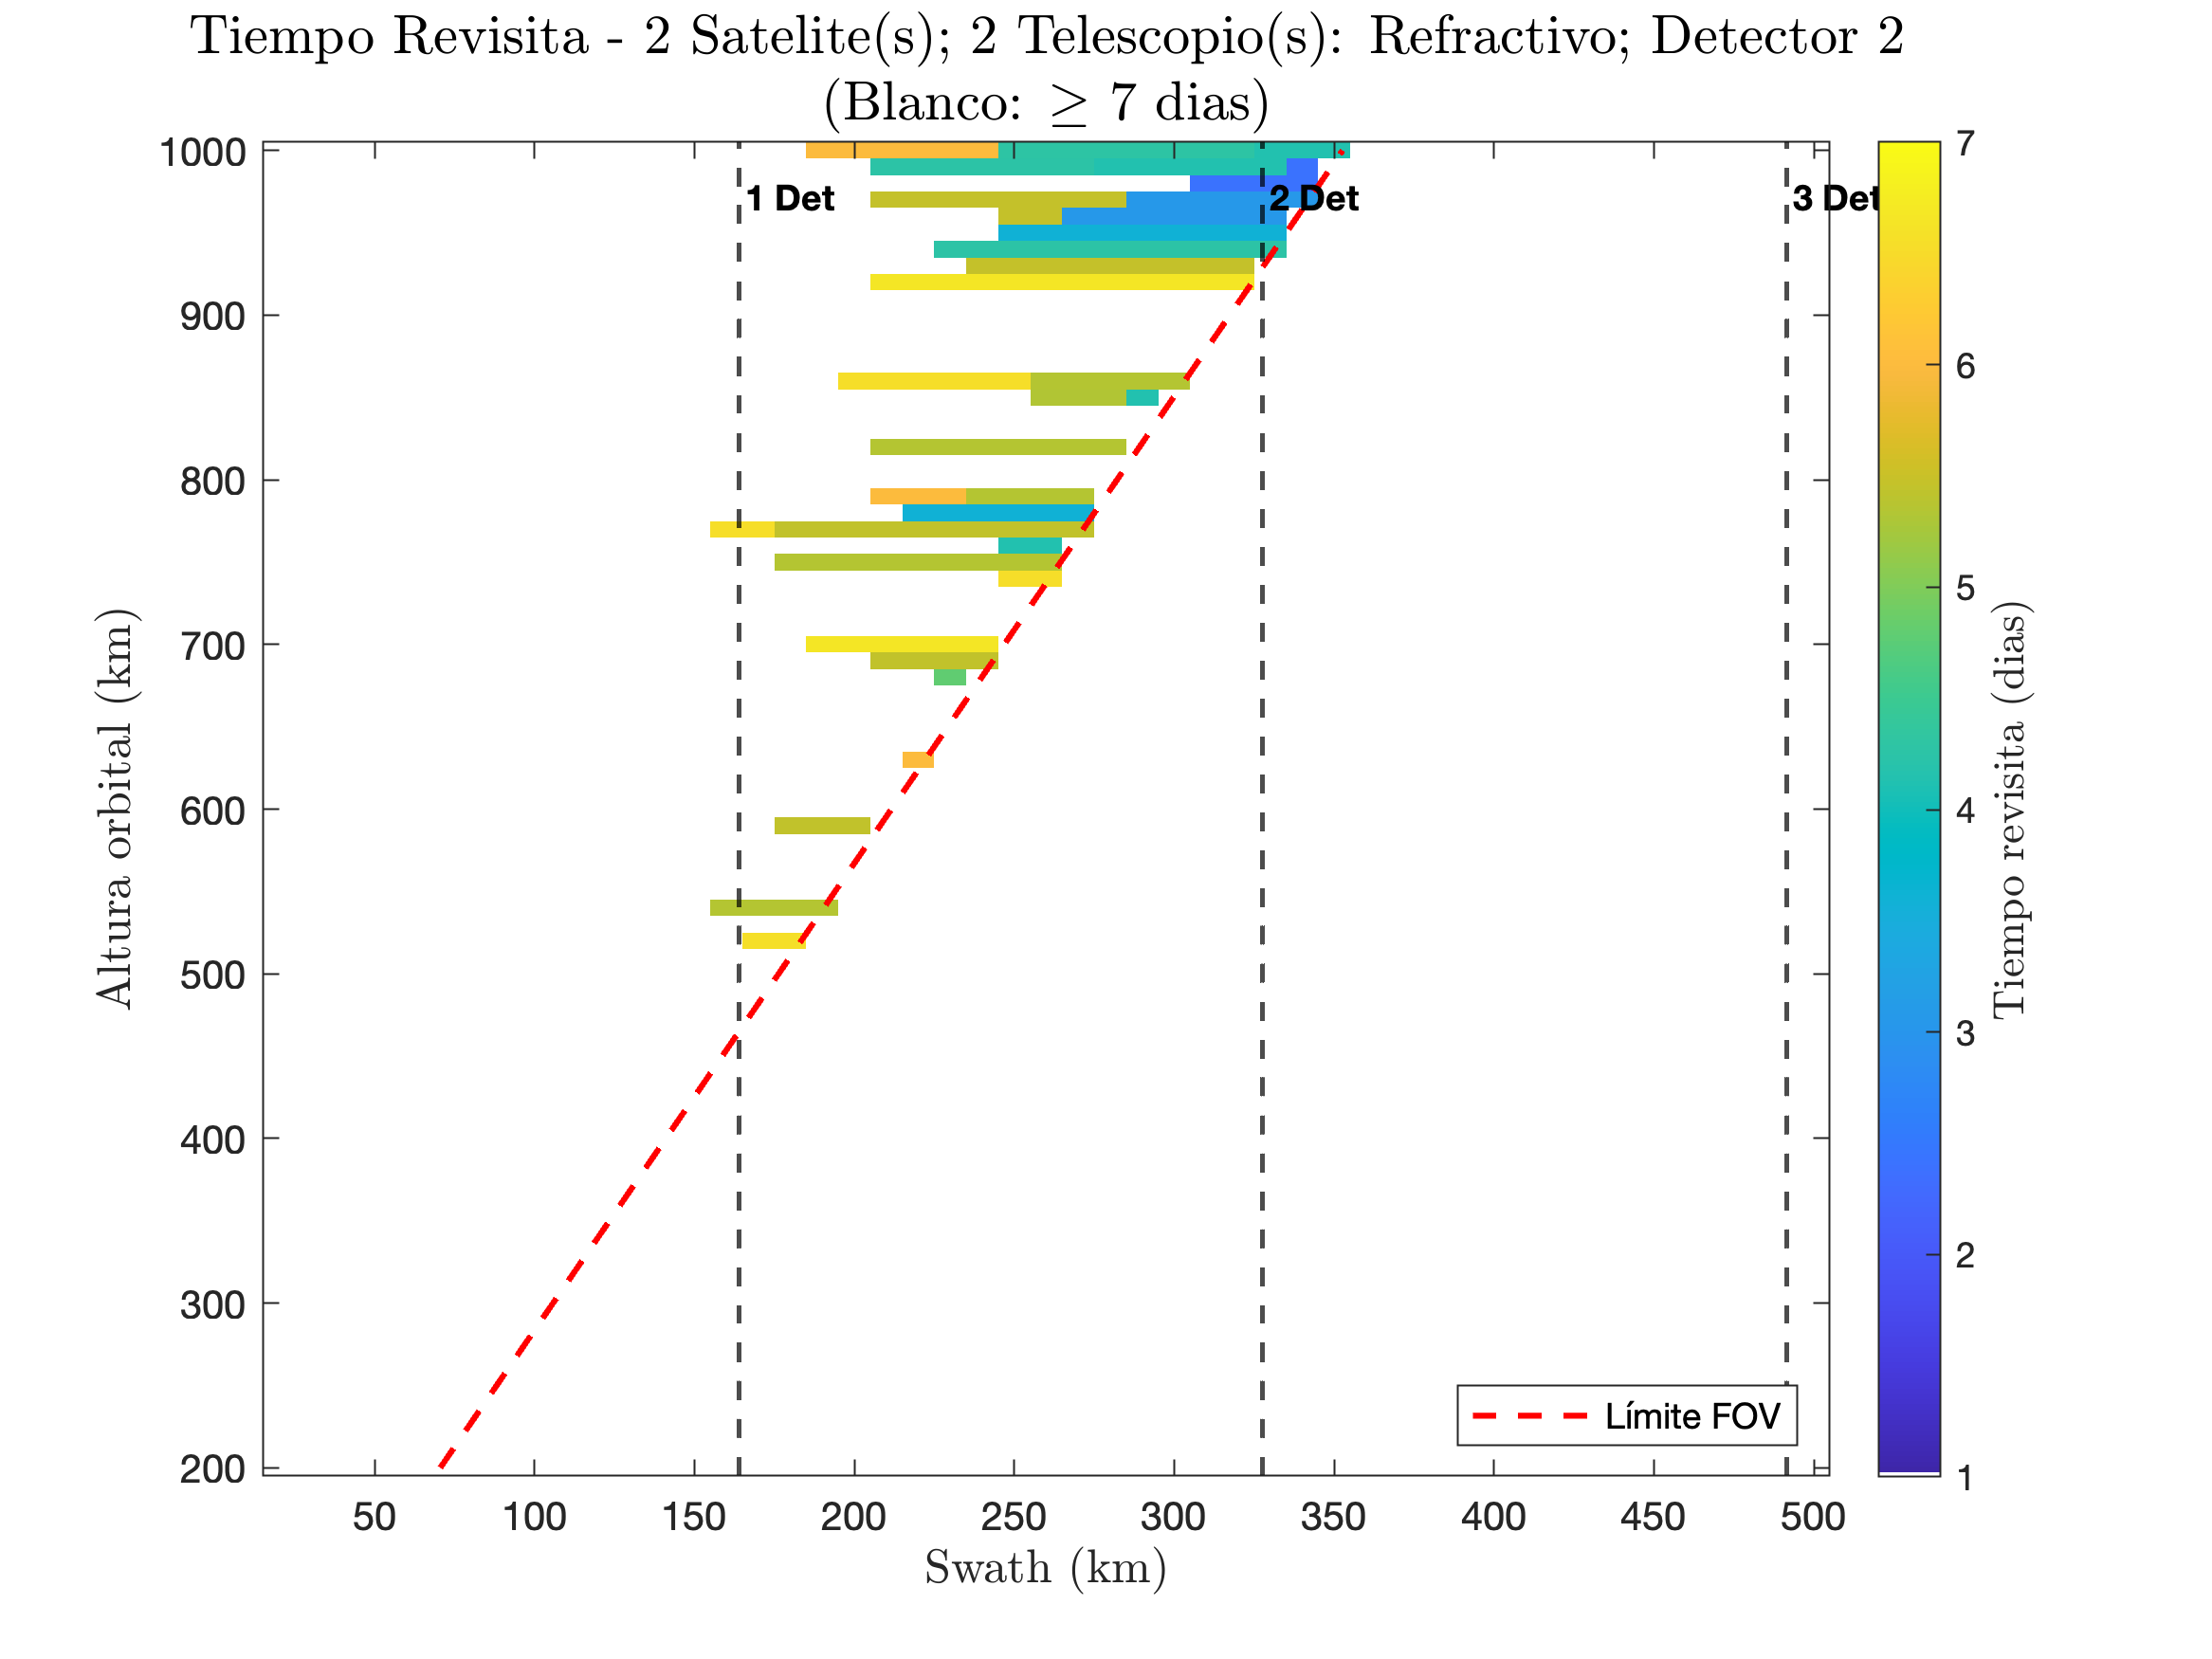
\includegraphics[width=0.48\linewidth]{4.Payload/Coverage/heatmap_2 Satelite(s); 2 Telescopio(s): Refractivo; Detector 2.jpg} &
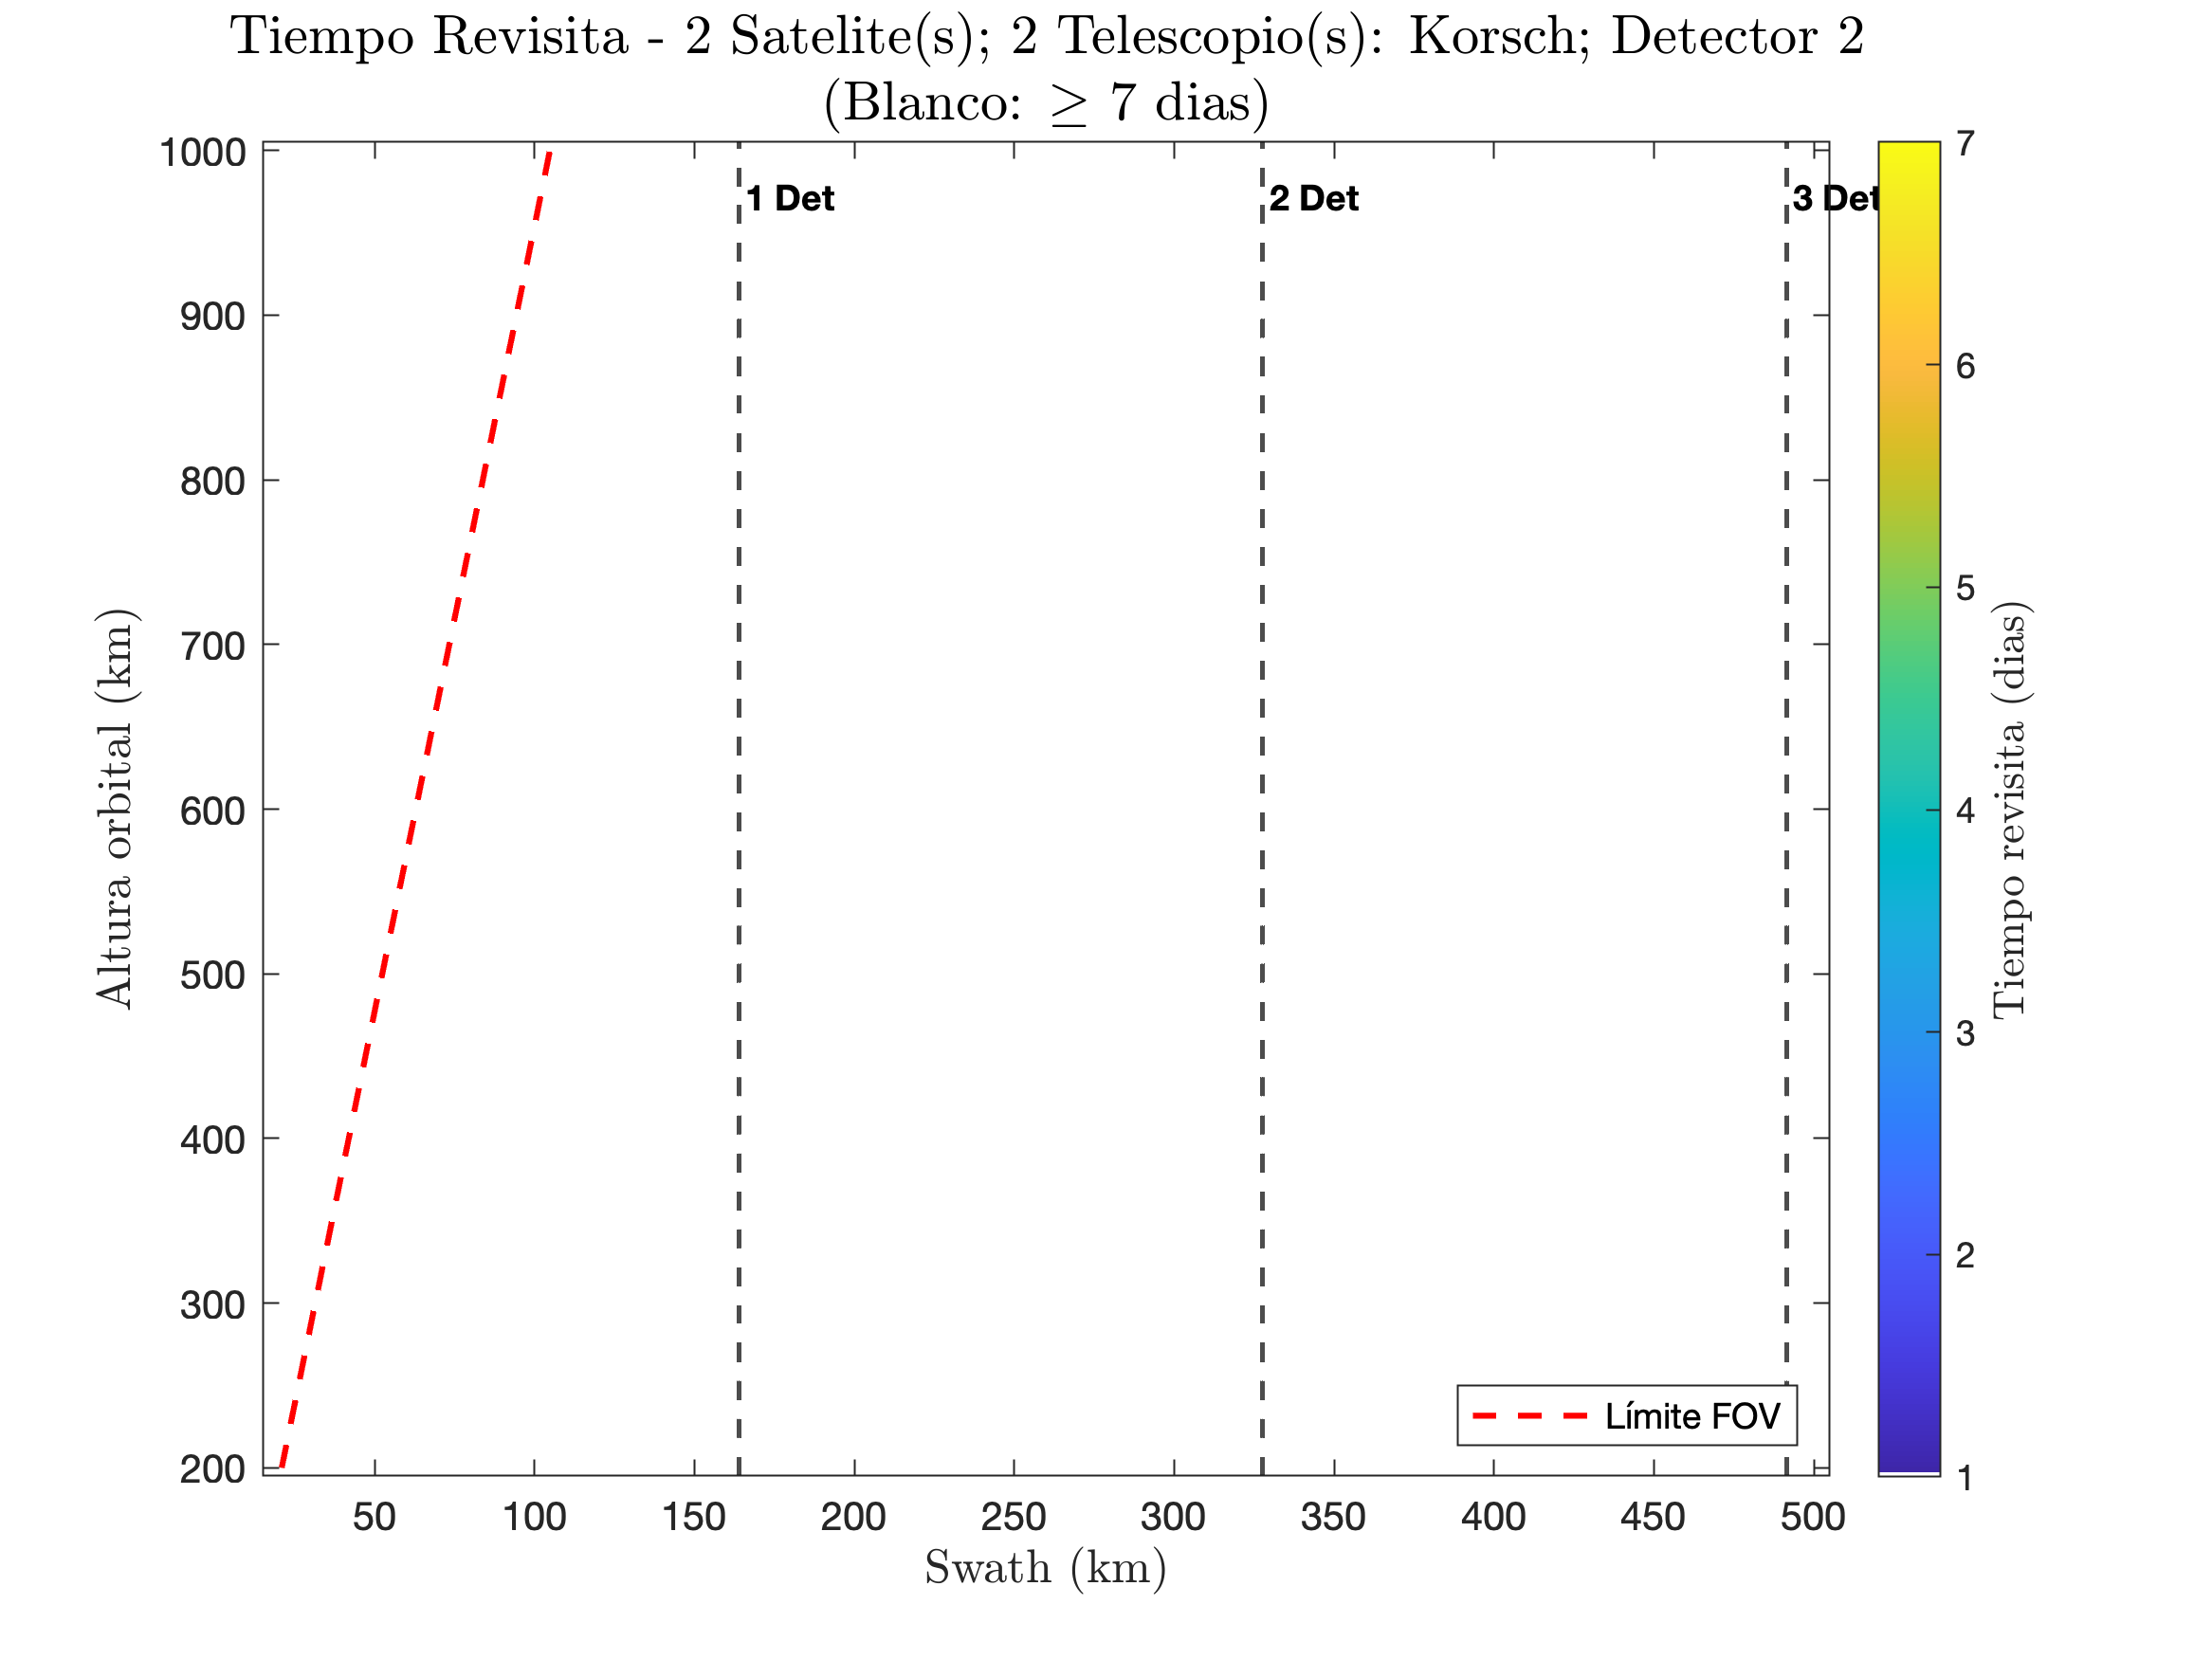
\includegraphics[width=0.48\linewidth]{4.Payload/Coverage/heatmap_2 Satelite(s); 2 Telescopio(s): Korsch; Detector 2.jpg} \\
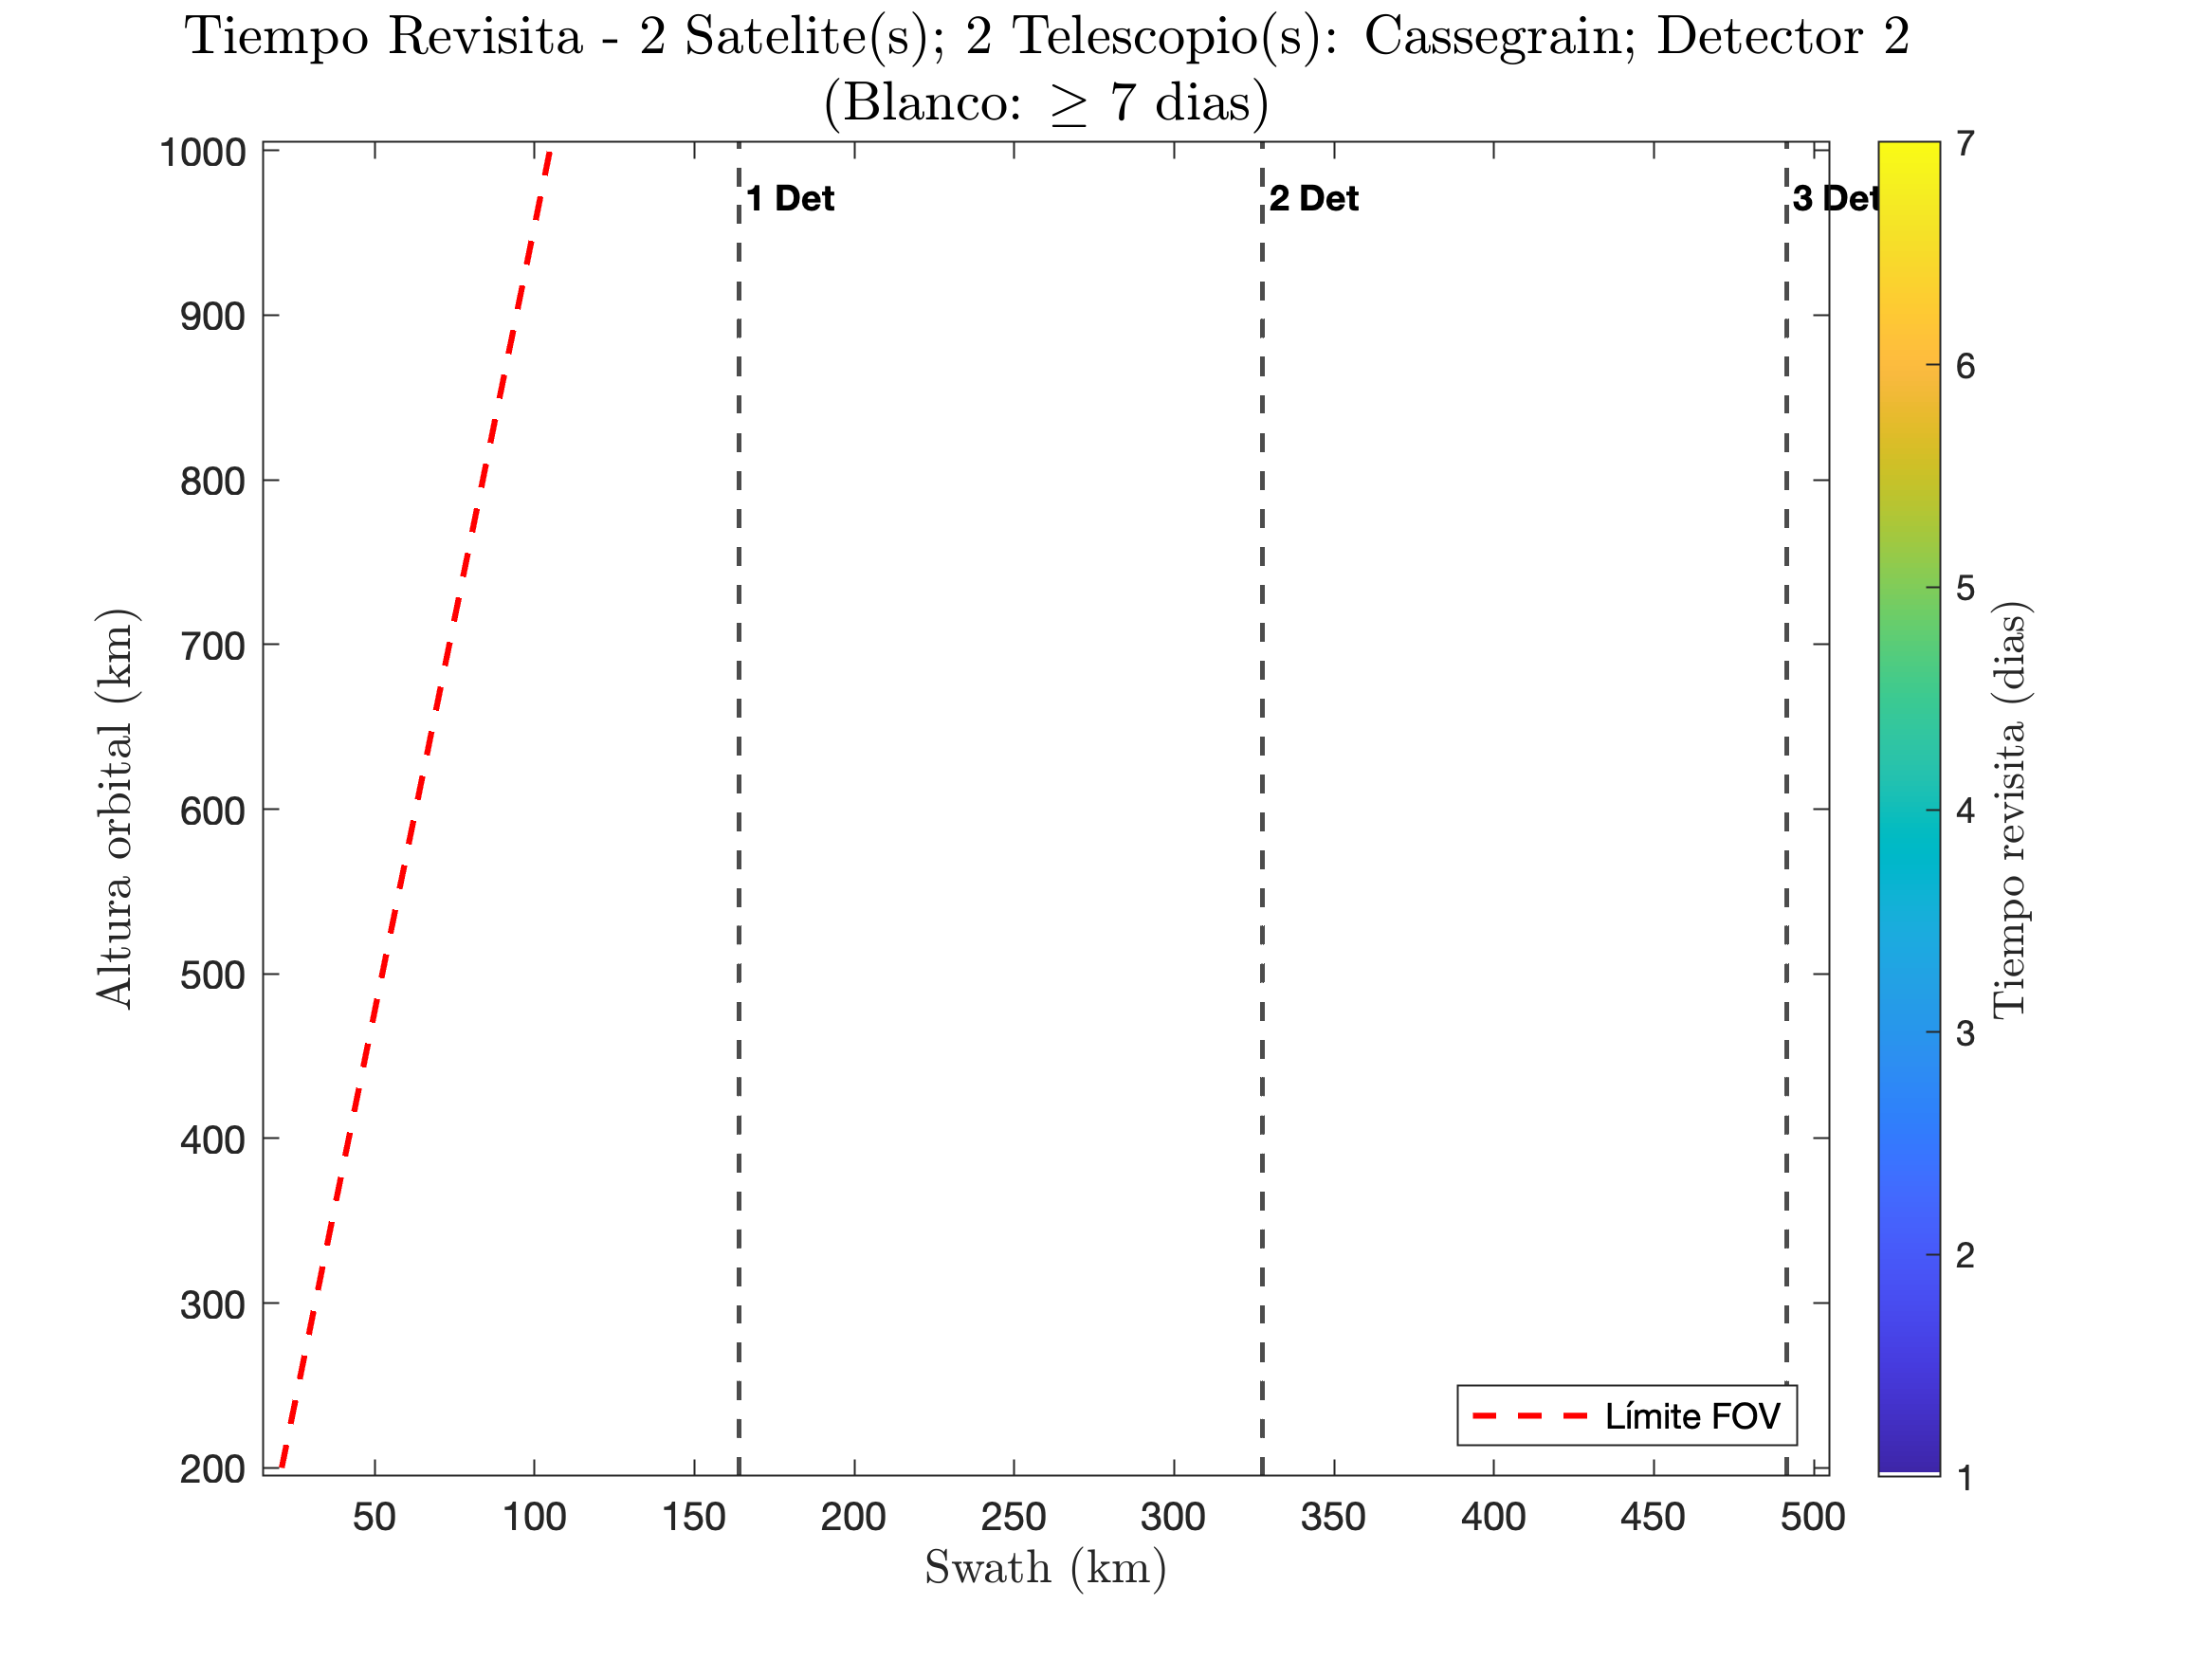
\includegraphics[width=0.48\linewidth]{4.Payload/Coverage/heatmap_2 Satelite(s); 2 Telescopio(s): Cassegrain; Detector 2.jpg} &
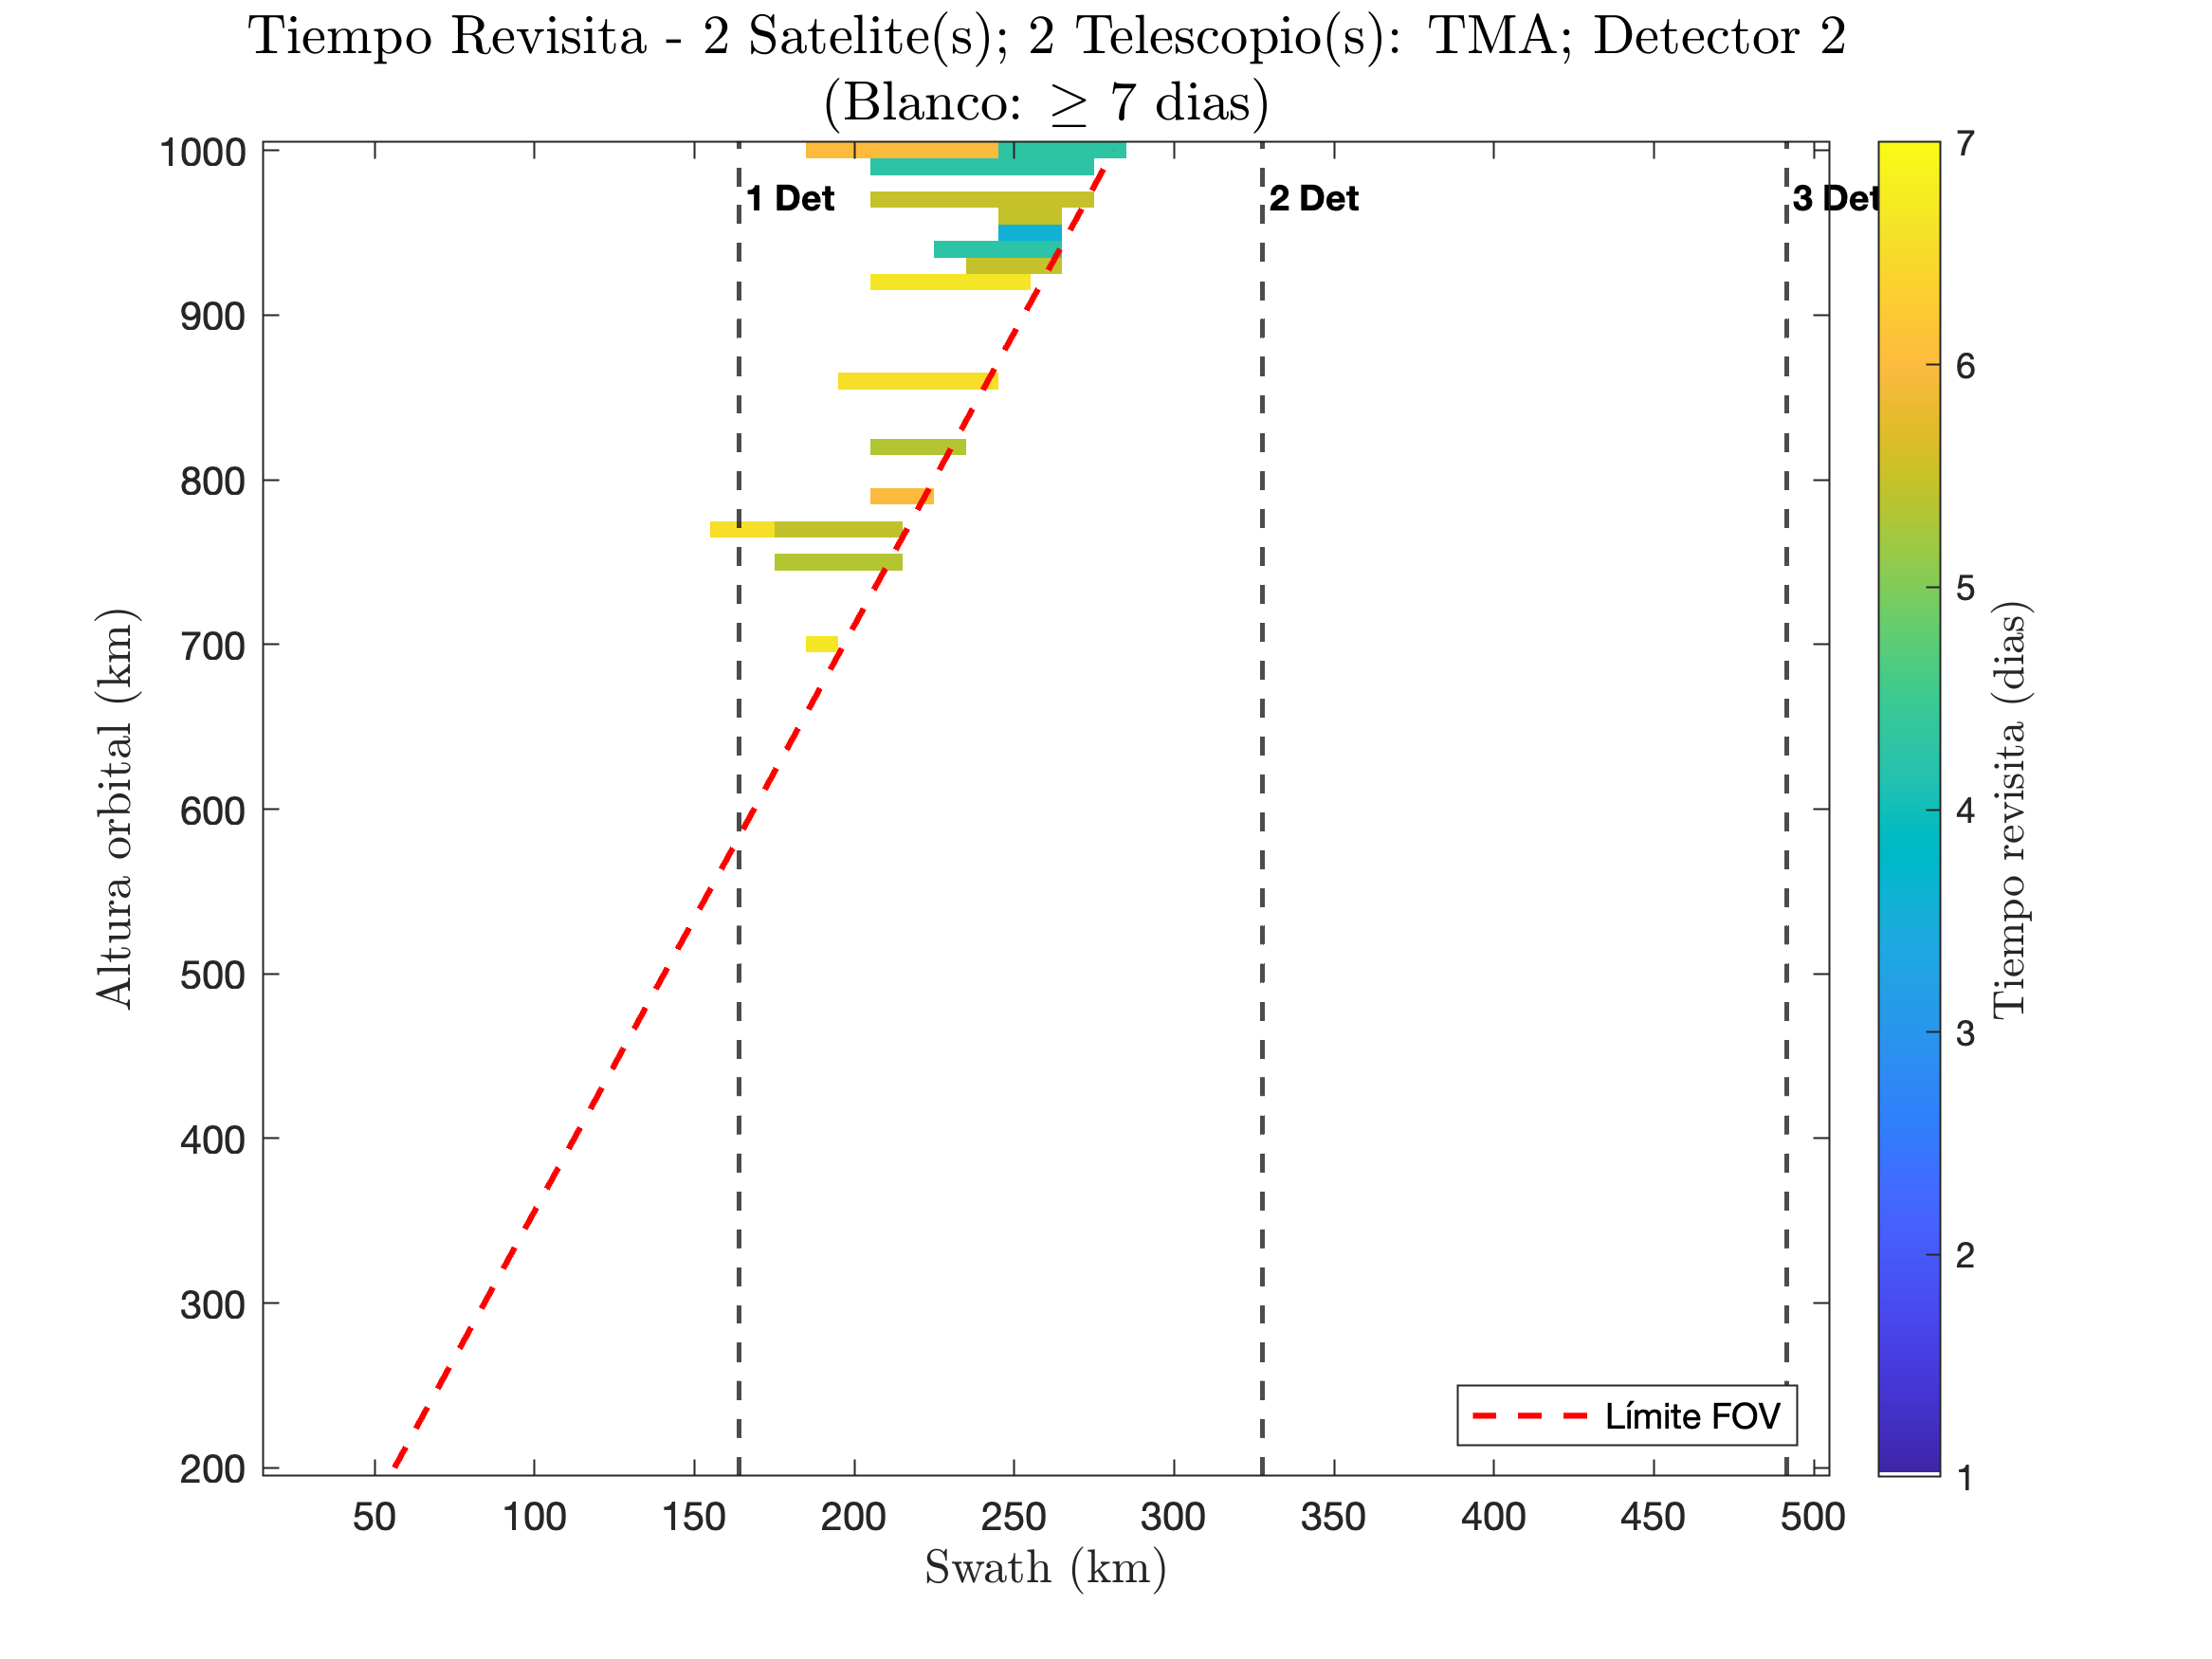
\includegraphics[width=0.48\linewidth]{4.Payload/Coverage/heatmap_2 Satelite(s); 2 Telescopio(s): TMA; Detector 2.jpg} \\
\end{tabular}
\caption{Mapas de calor resultantes del cálculo de cobertura para el Detector 2, con 2 satélites y 2 telescopios.}
\end{figure}
\end{landscape}

\begin{landscape}
\begin{figure}[p]
\centering
\vspace*{0.3cm}
\setlength{\tabcolsep}{4pt}
\renewcommand{\arraystretch}{0}
\begin{tabular}{cc}
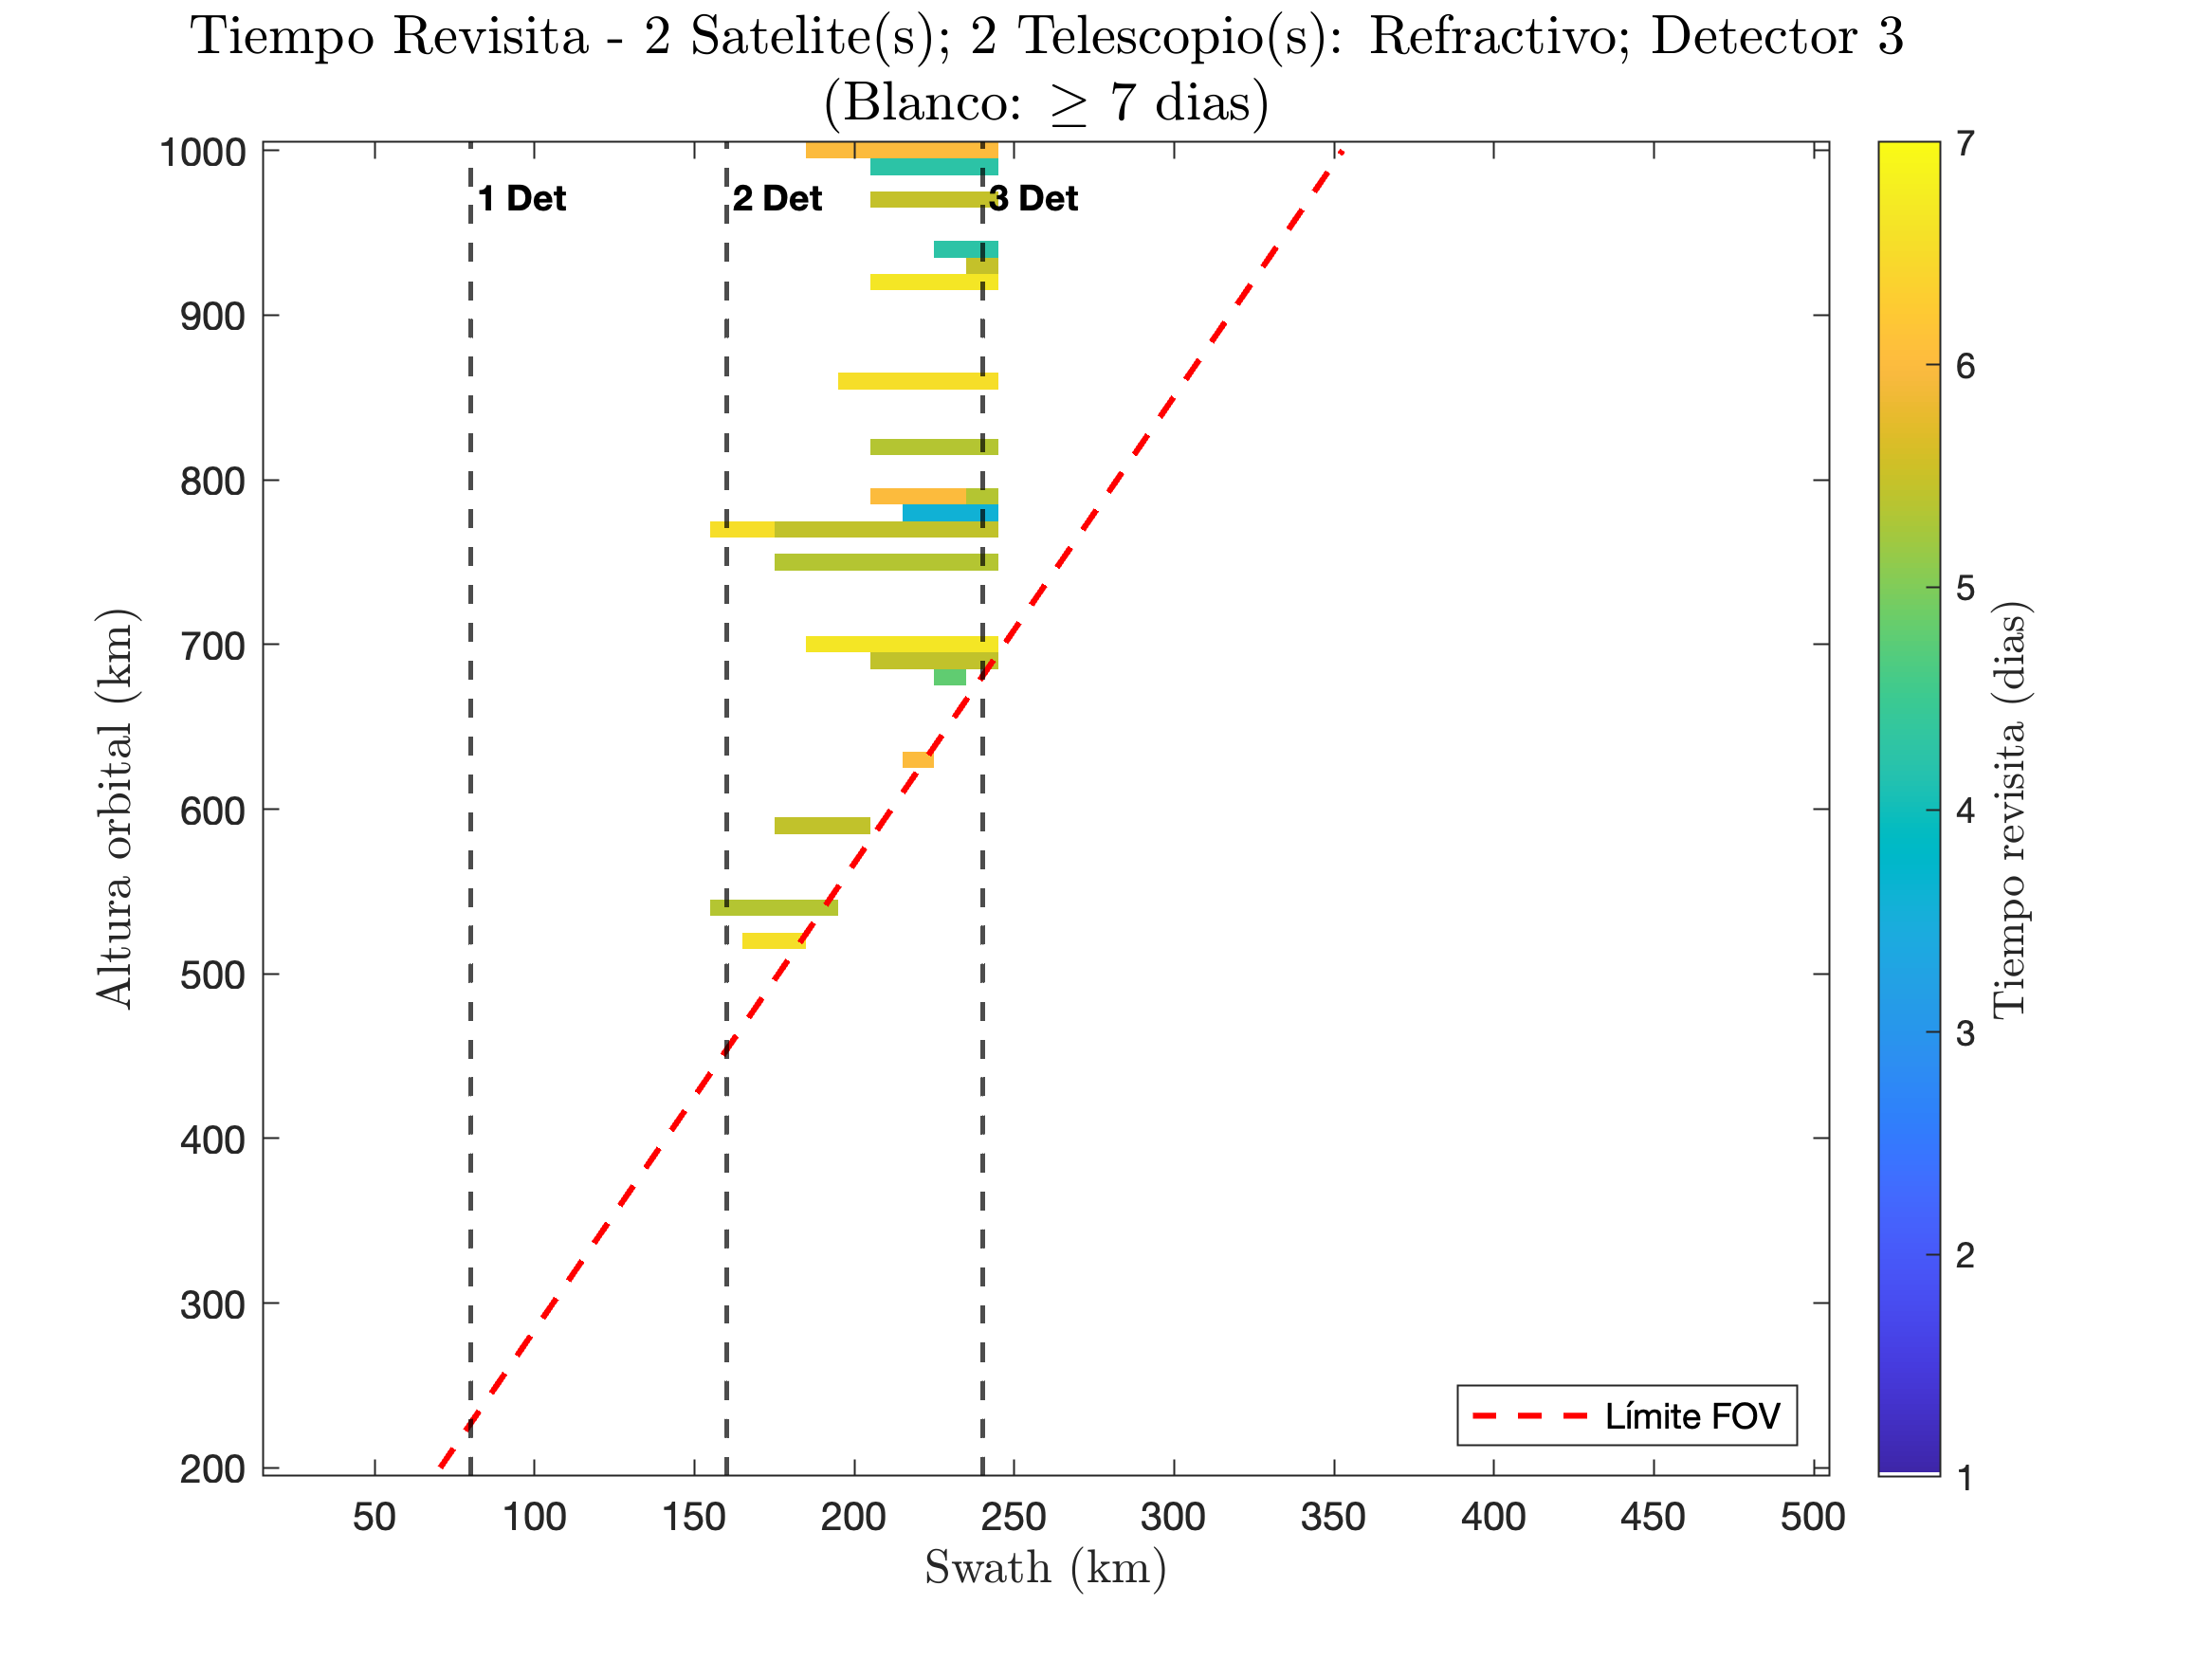
\includegraphics[width=0.48\linewidth]{4.Payload/Coverage/heatmap_2 Satelite(s); 2 Telescopio(s): Refractivo; Detector 3.jpg} &
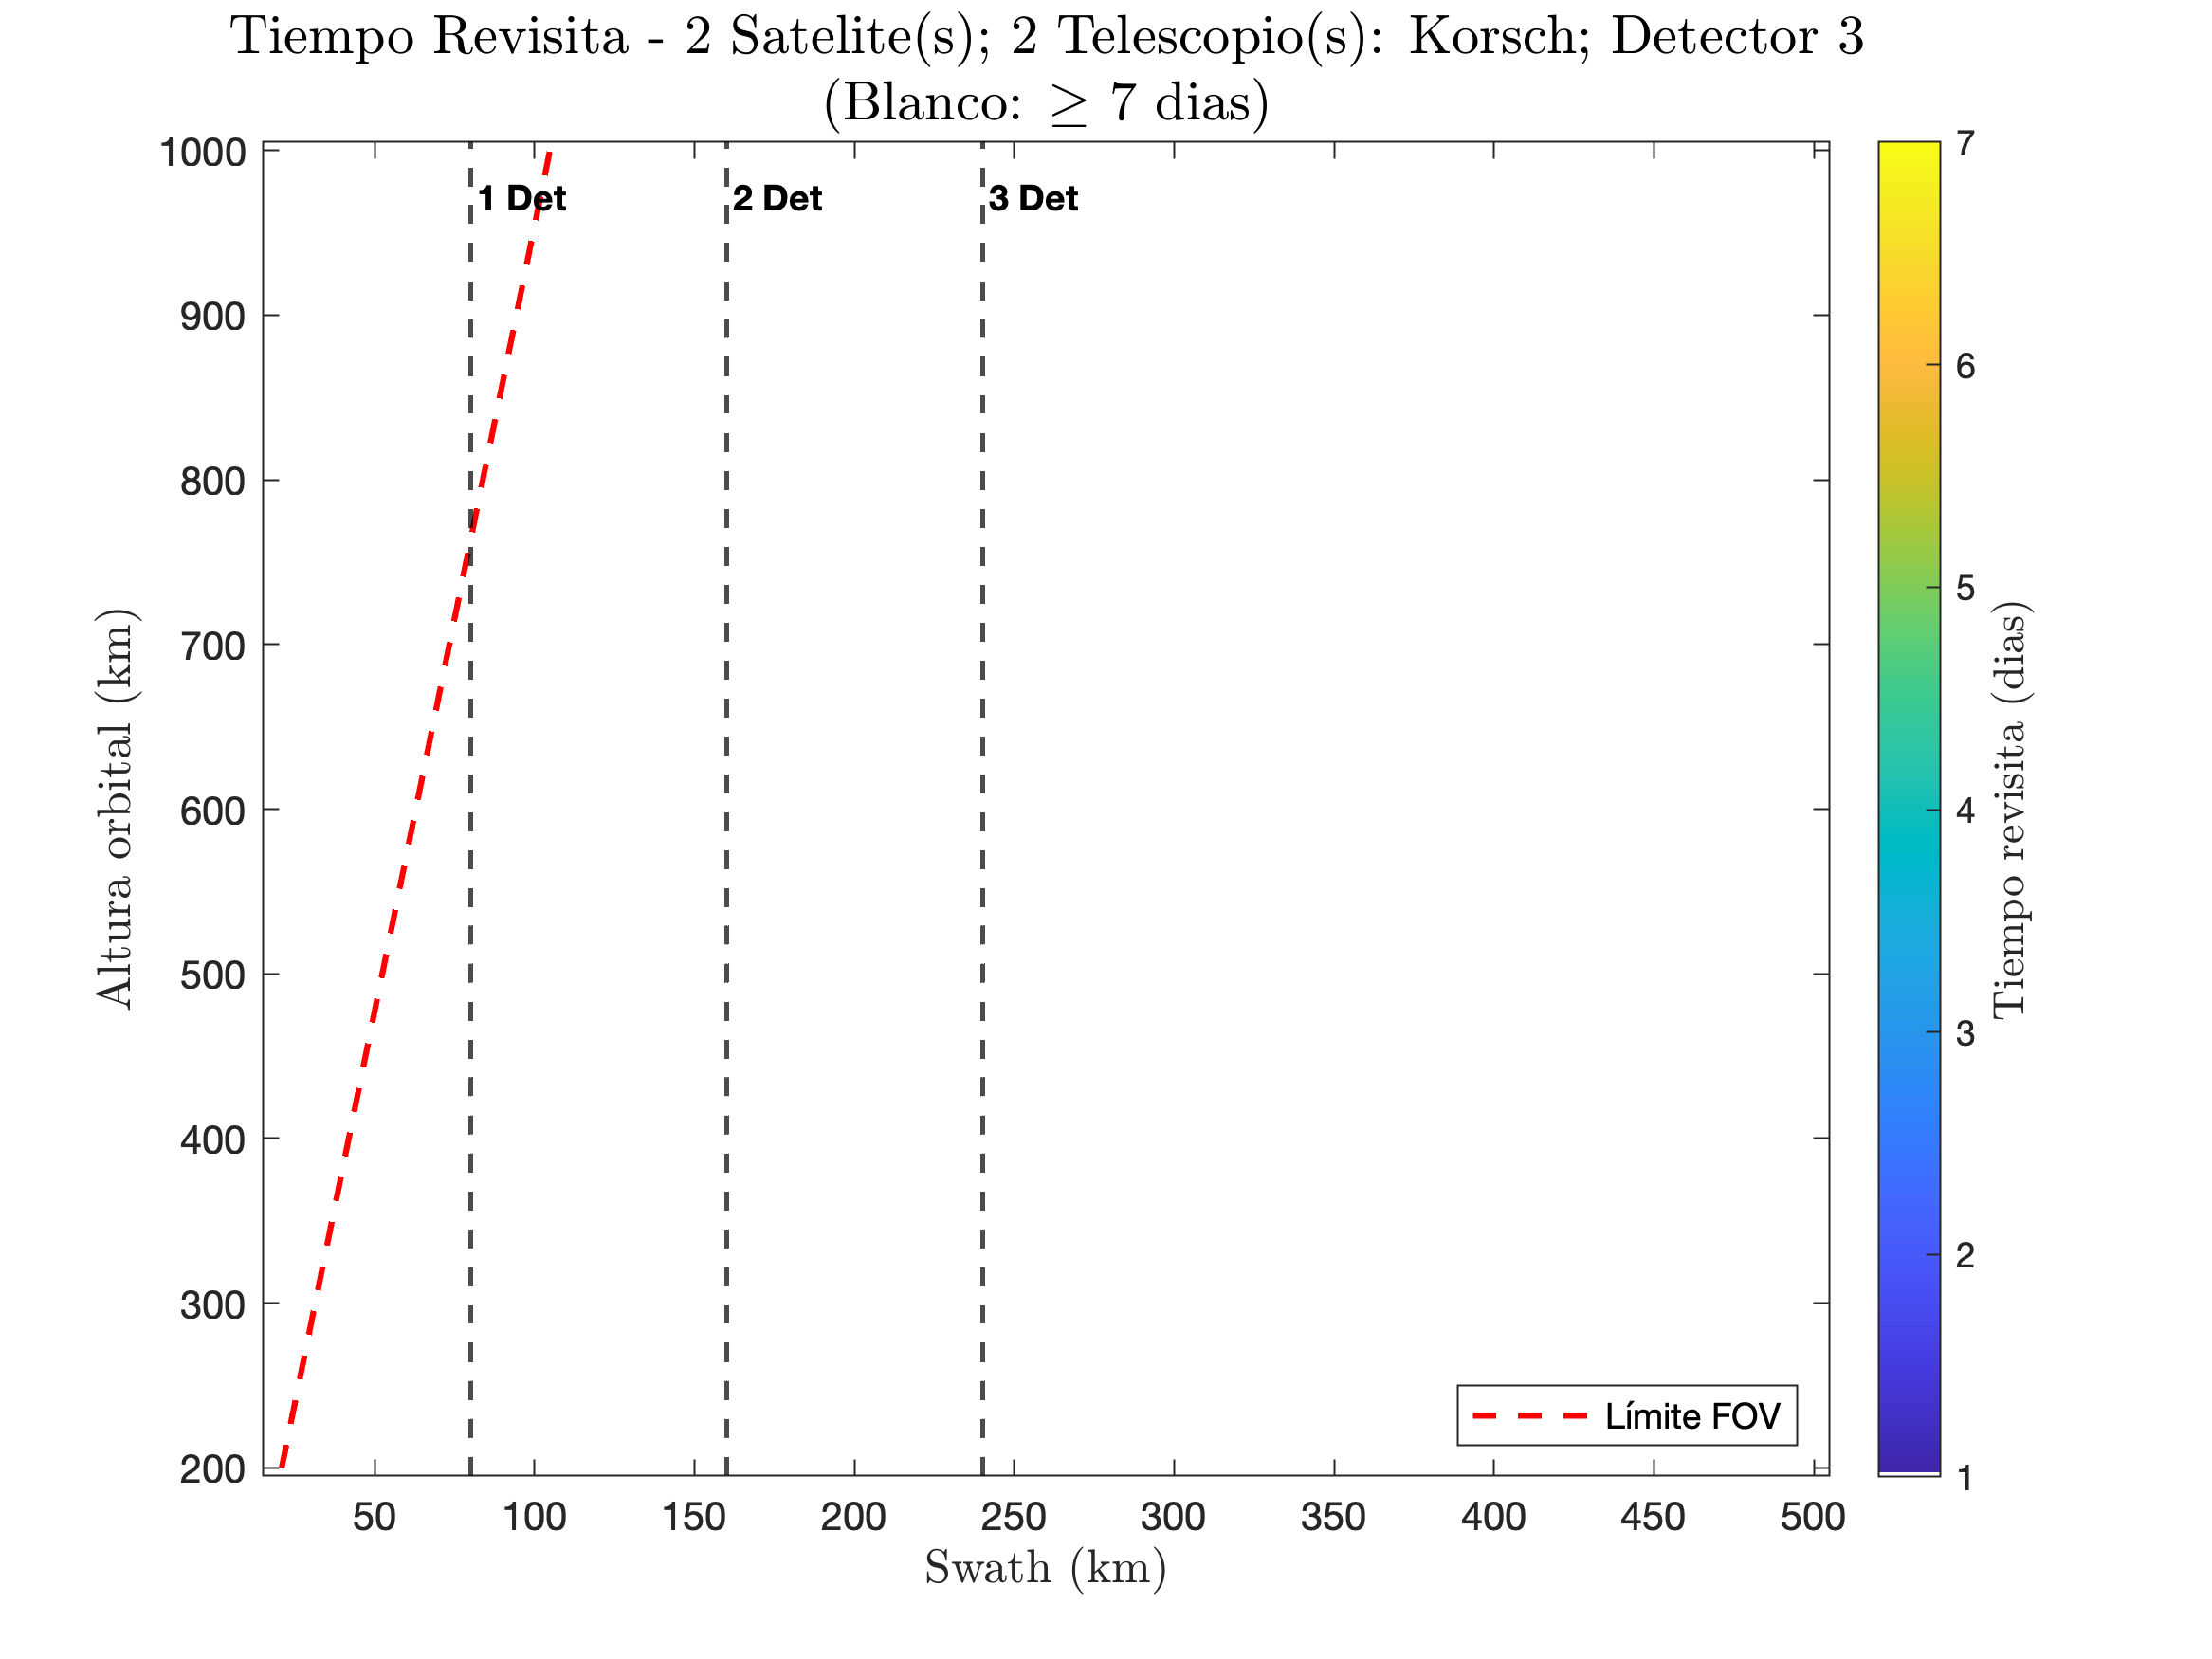
\includegraphics[width=0.48\linewidth]{4.Payload/Coverage/heatmap_2 Satelite(s); 2 Telescopio(s): Korsch; Detector 3.jpg} \\
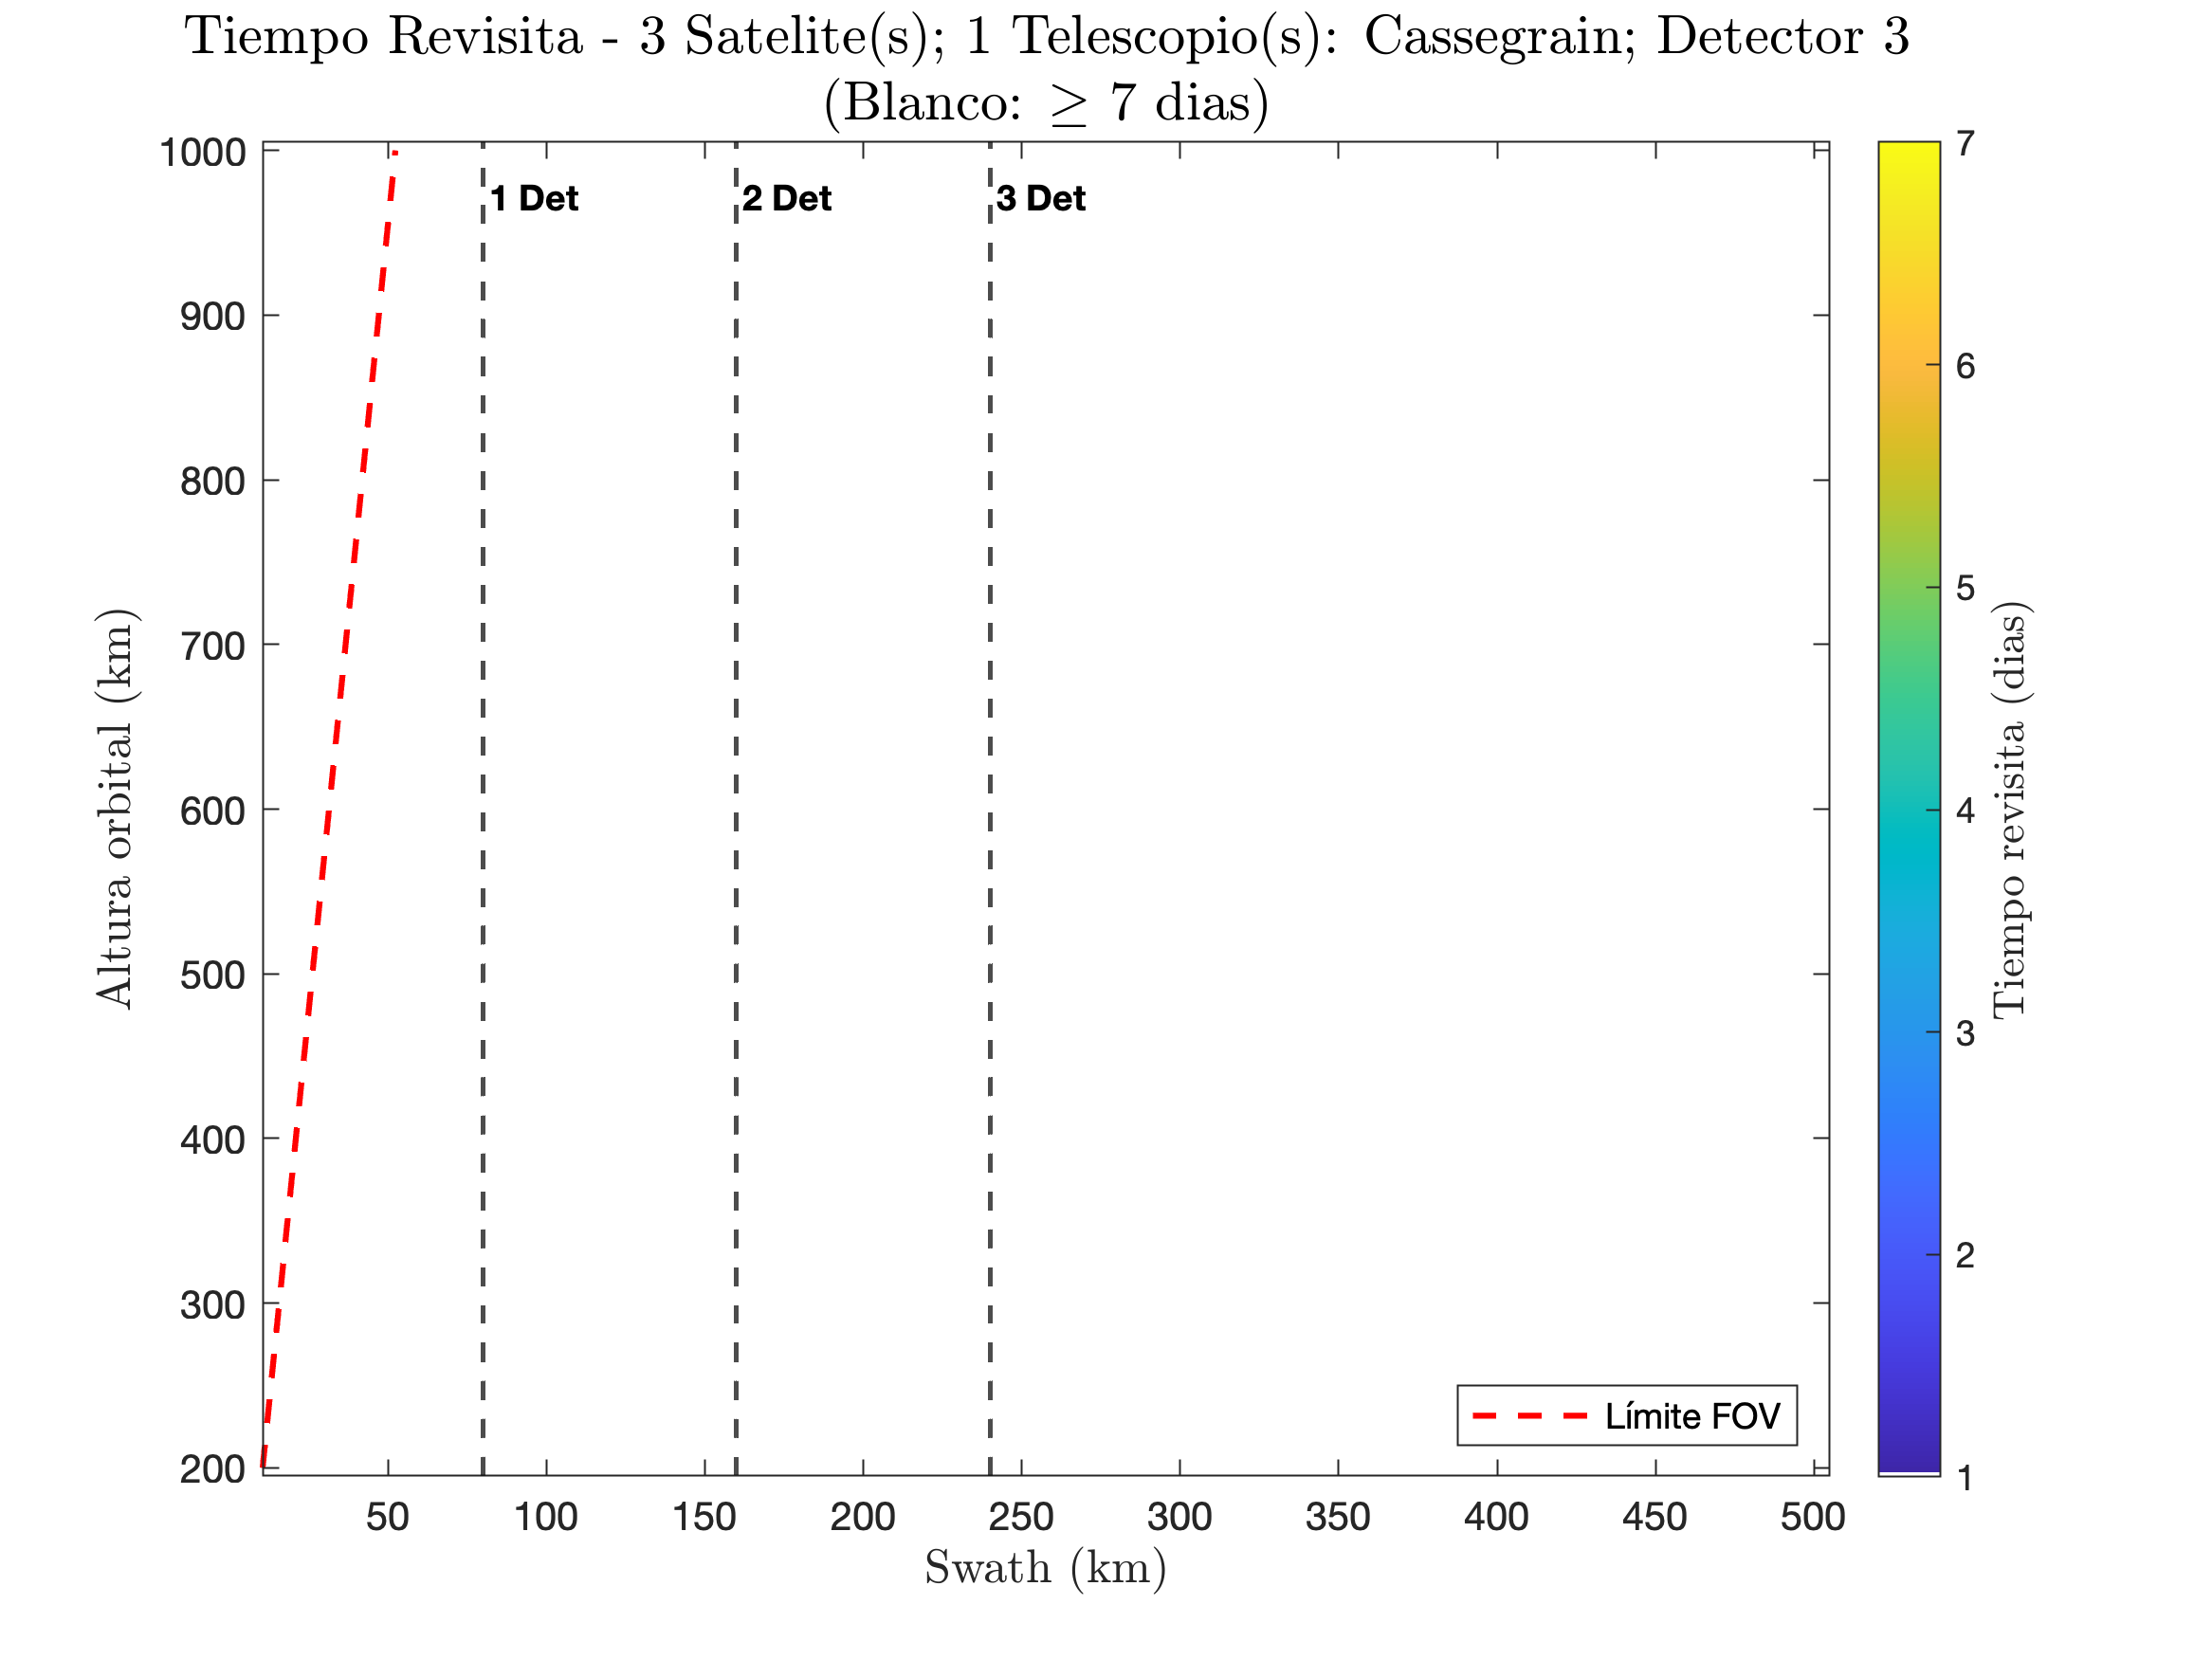
\includegraphics[width=0.48\linewidth]{4.Payload/Coverage/heatmap_3 Satelite(s); 1 Telescopio(s): Cassegrain; Detector 3.jpg} &
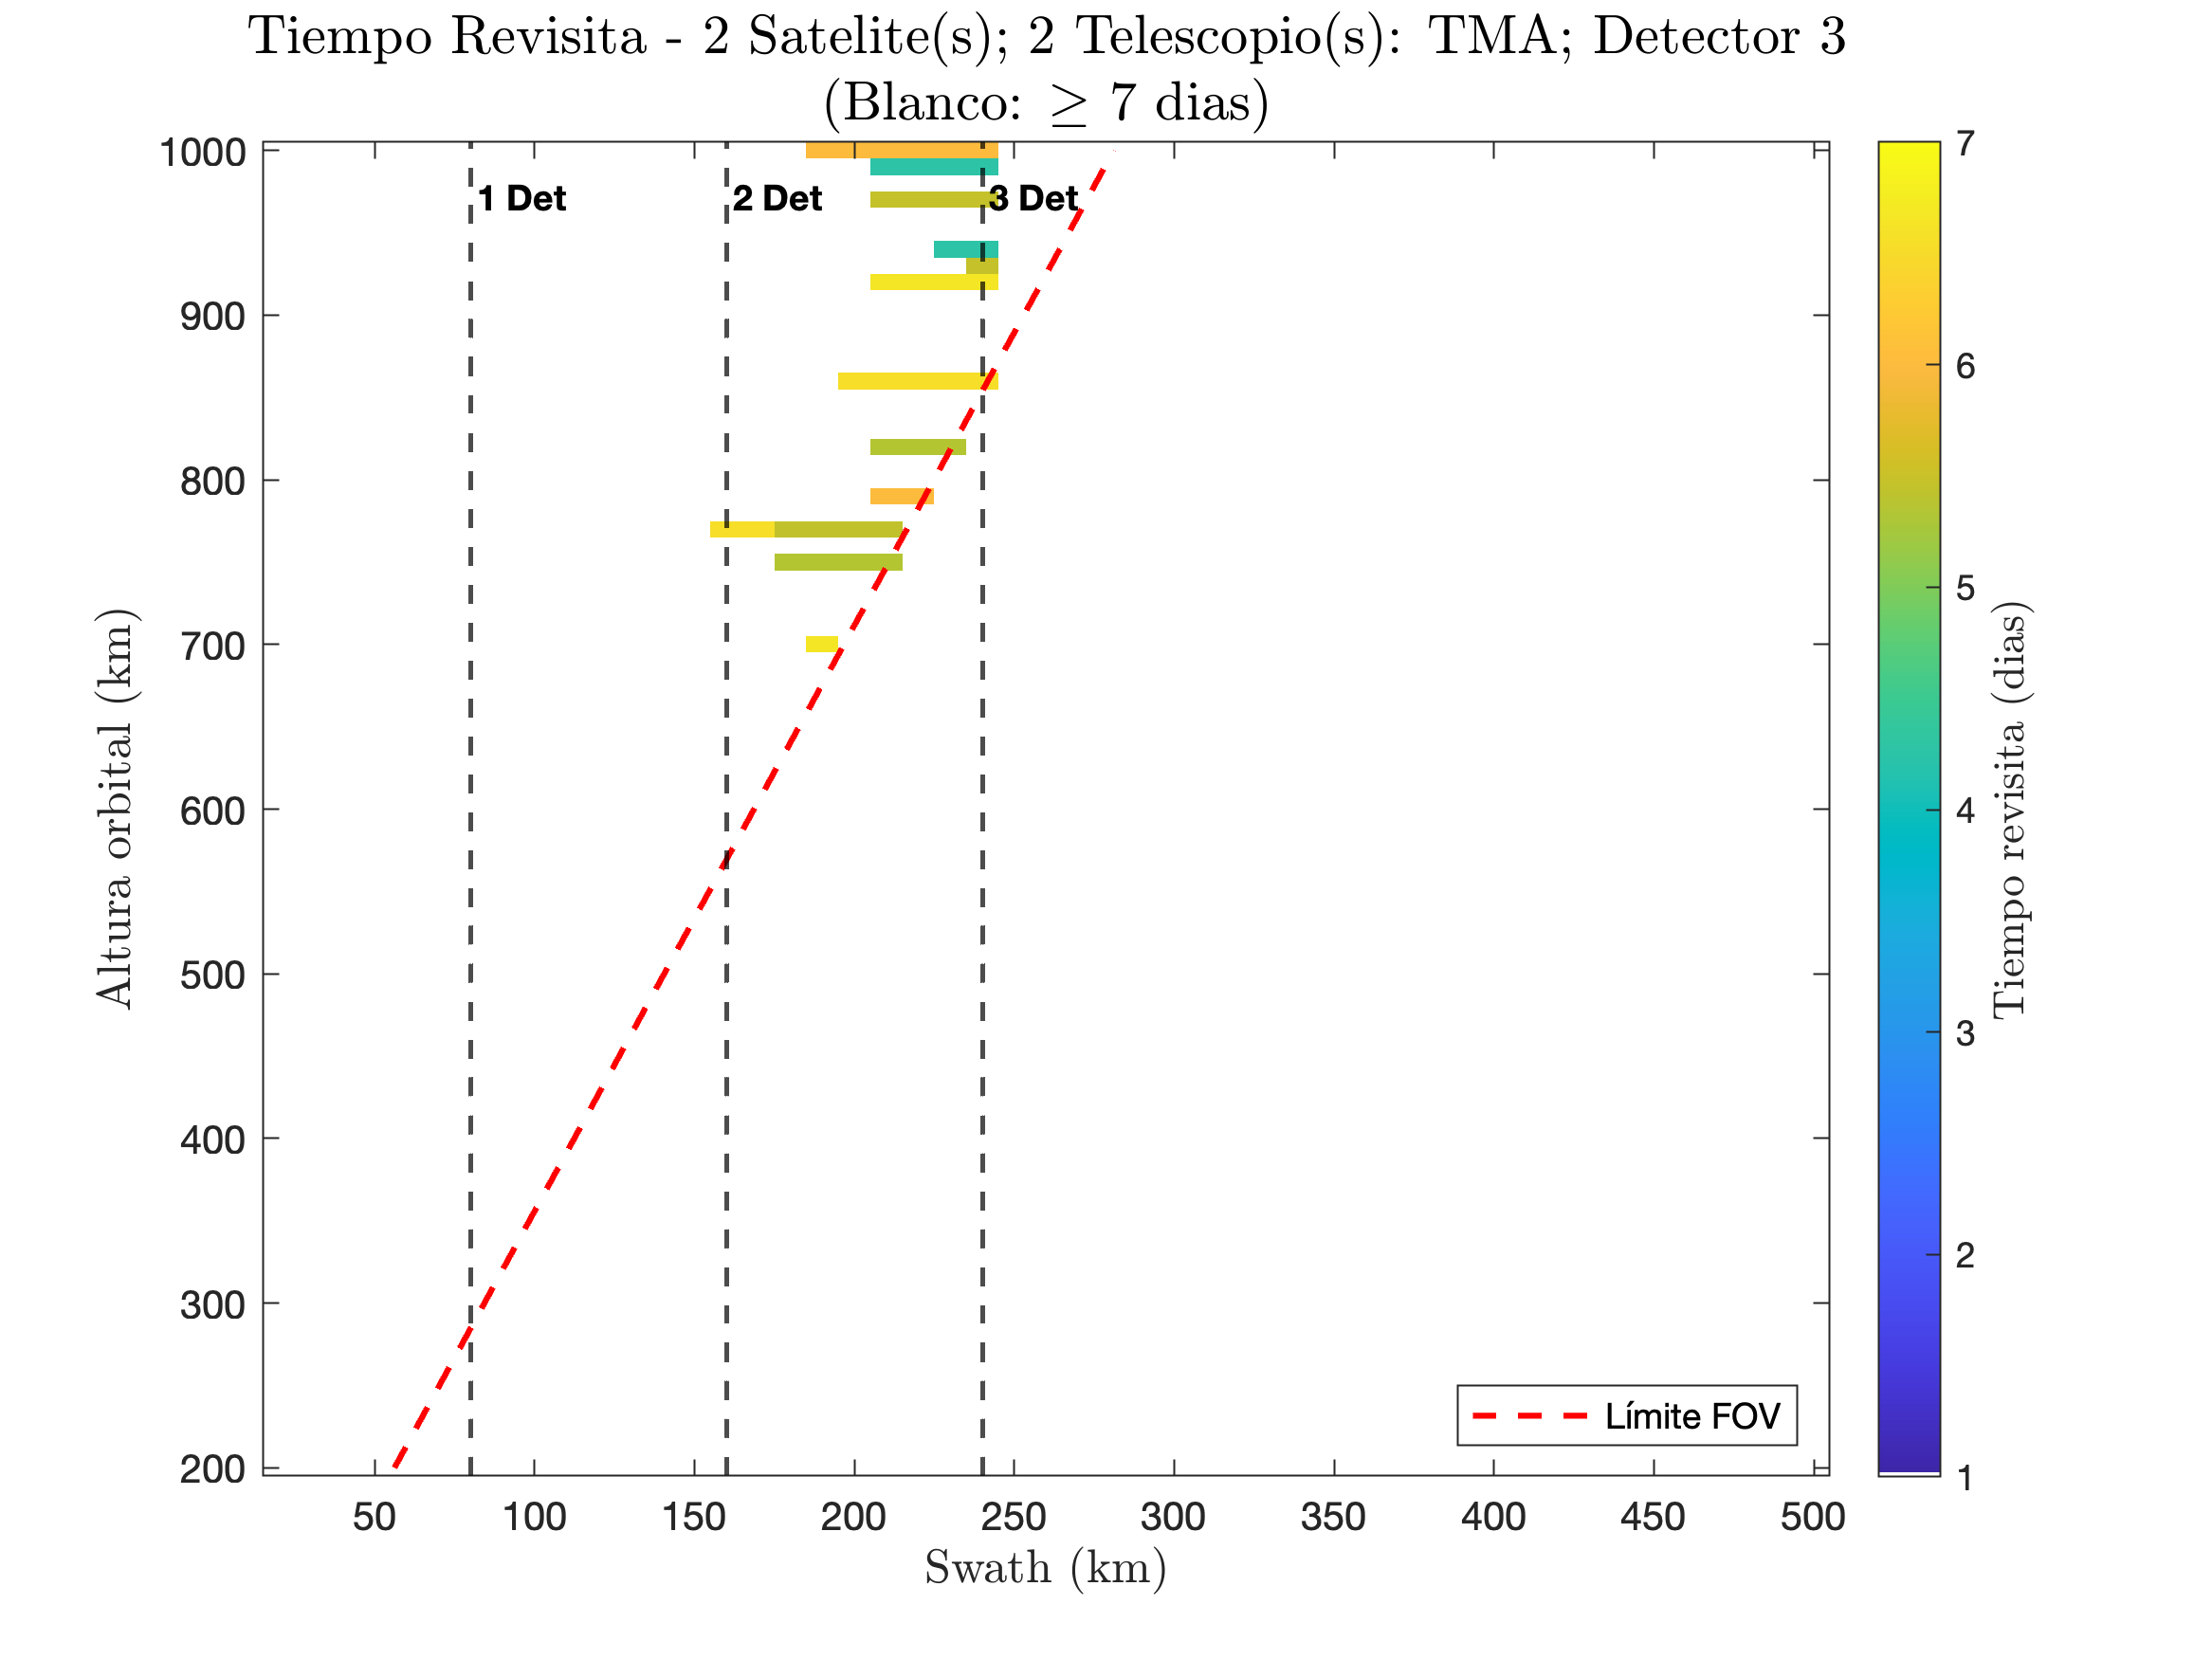
\includegraphics[width=0.48\linewidth]{4.Payload/Coverage/heatmap_2 Satelite(s); 2 Telescopio(s): TMA; Detector 3.jpg} \\
\end{tabular}
\caption{Mapas de calor resultantes del cálculo de cobertura para el Detector 3, con 2 satélites y 2 telescopios.}
\end{figure}
\end{landscape}


%% Graficas 3 SAT
\begin{landscape}
\begin{figure}[p]
\centering
\vspace*{0.3cm}
\setlength{\tabcolsep}{4pt}
\renewcommand{\arraystretch}{0}
\begin{tabular}{cc}
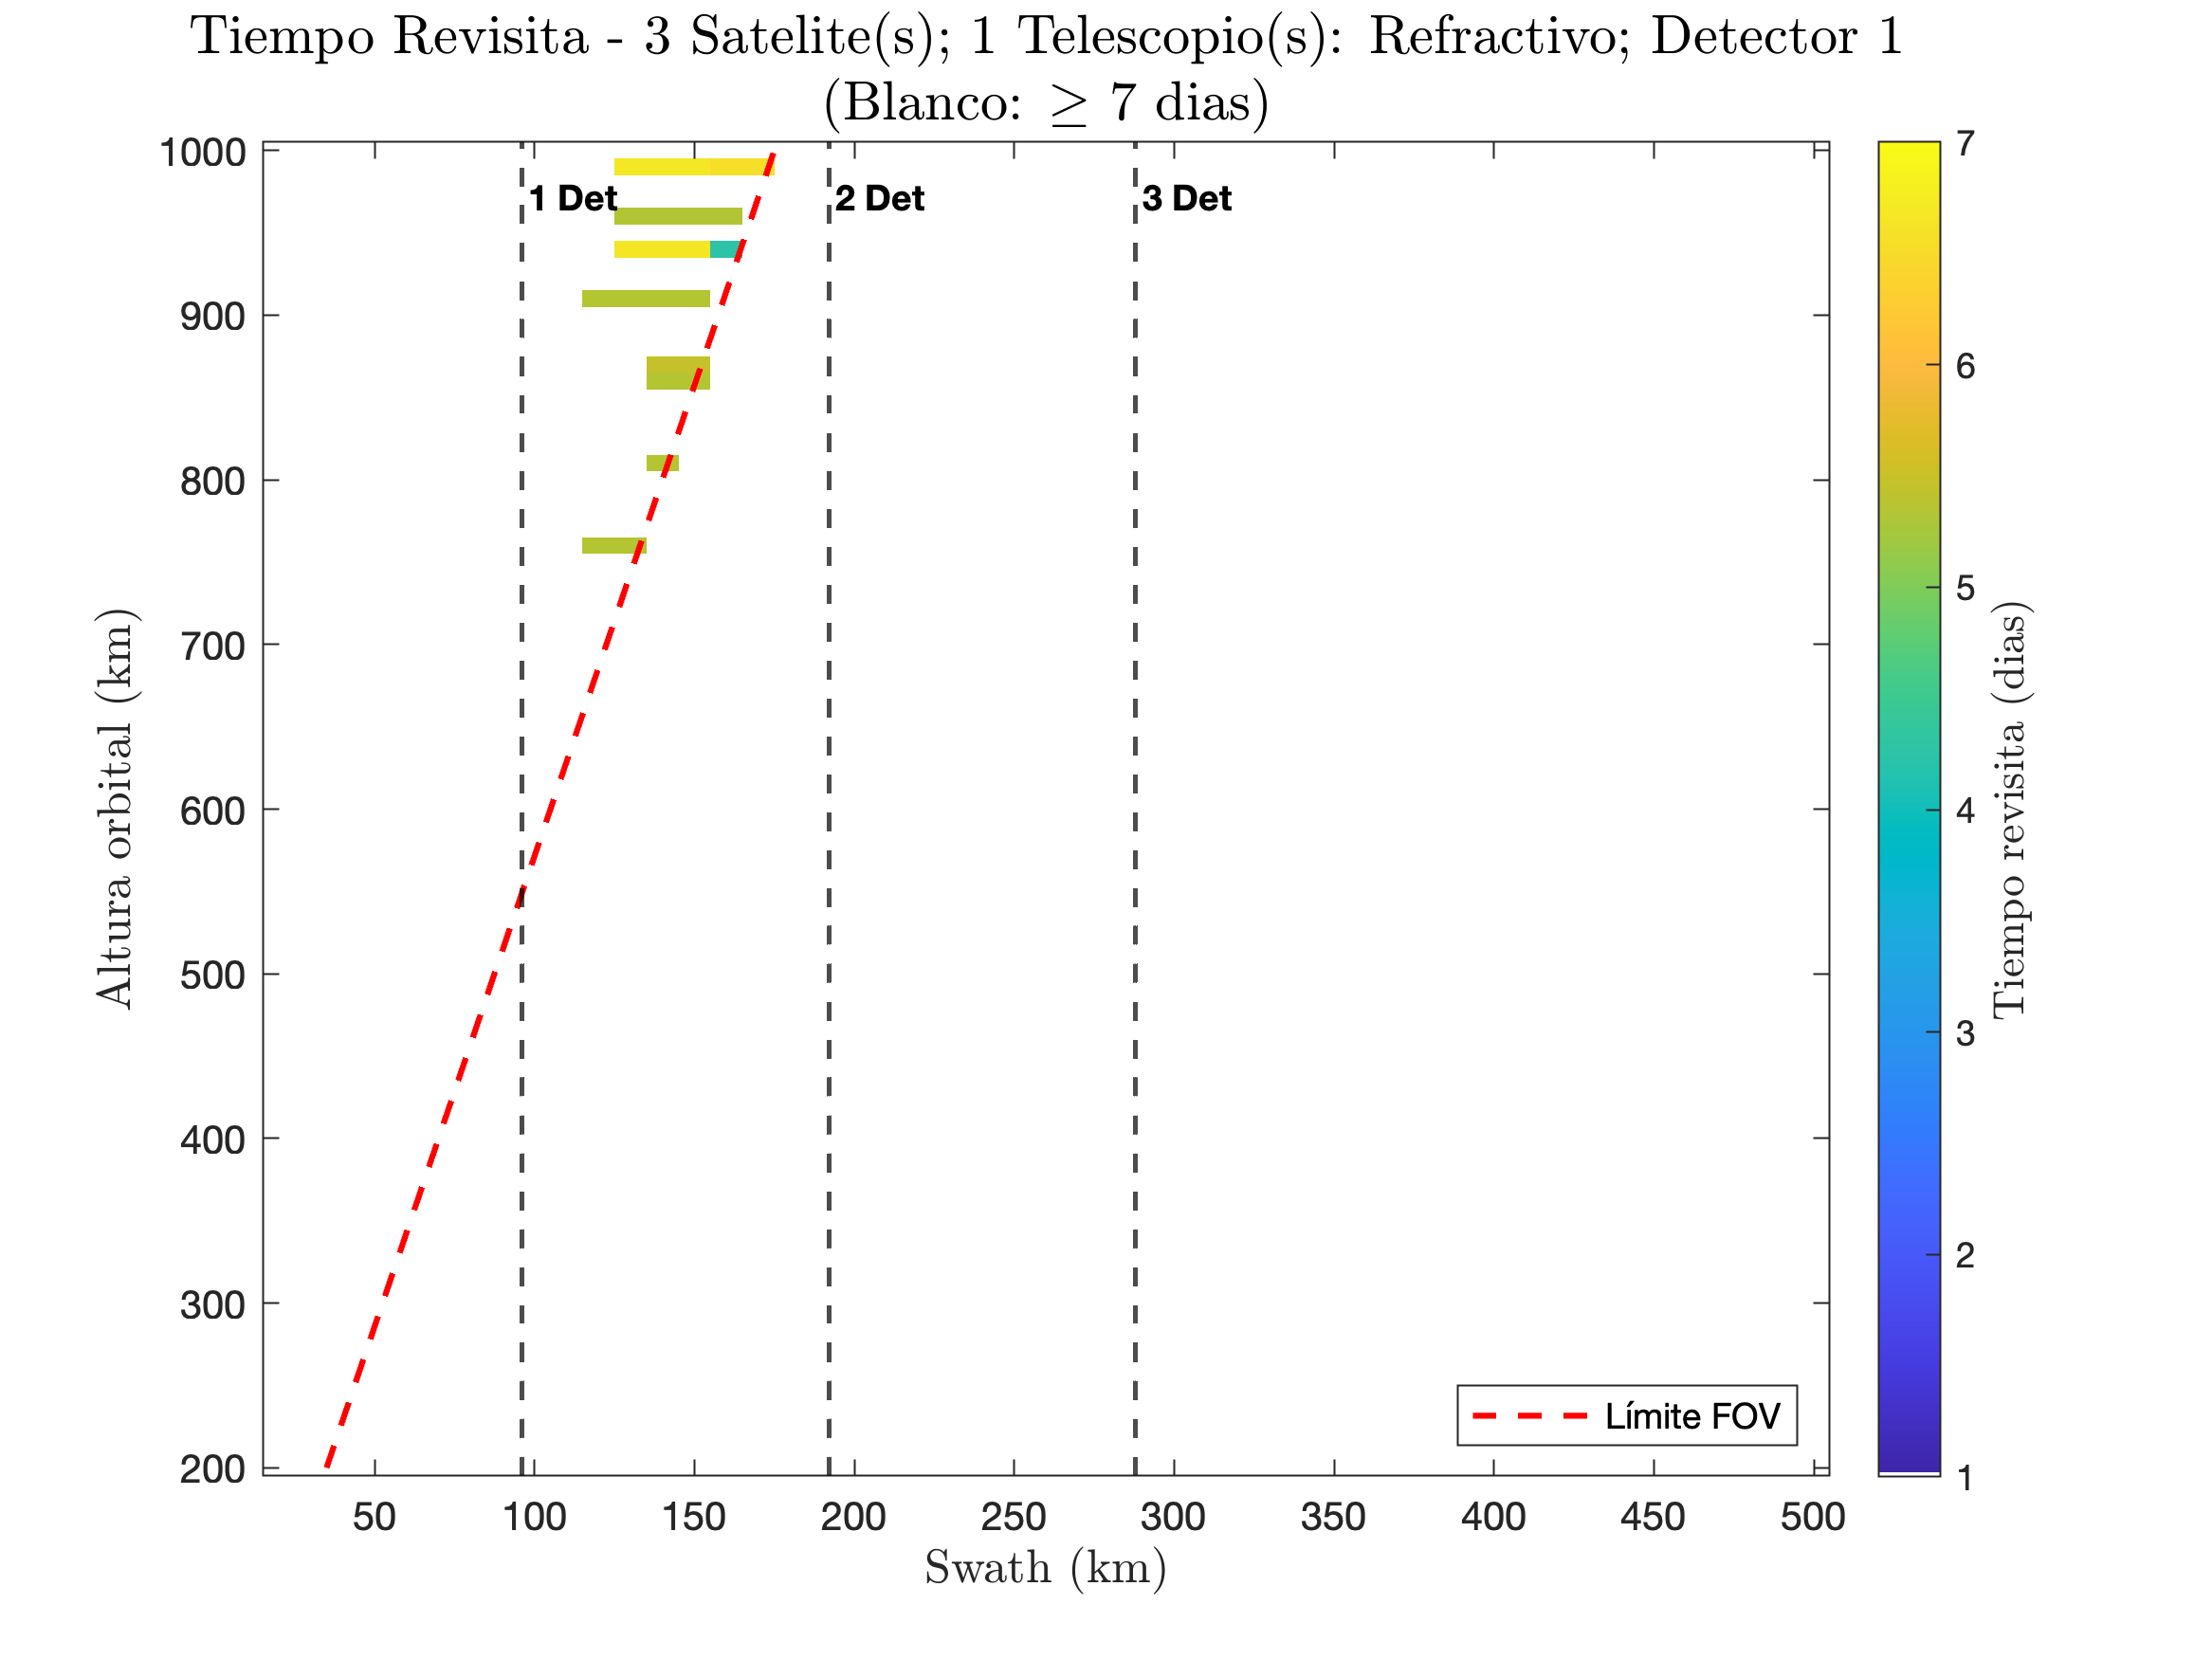
\includegraphics[width=0.48\linewidth]{4.Payload/Coverage/heatmap_3 Satelite(s); 1 Telescopio(s): Refractivo; Detector 1.jpg} &
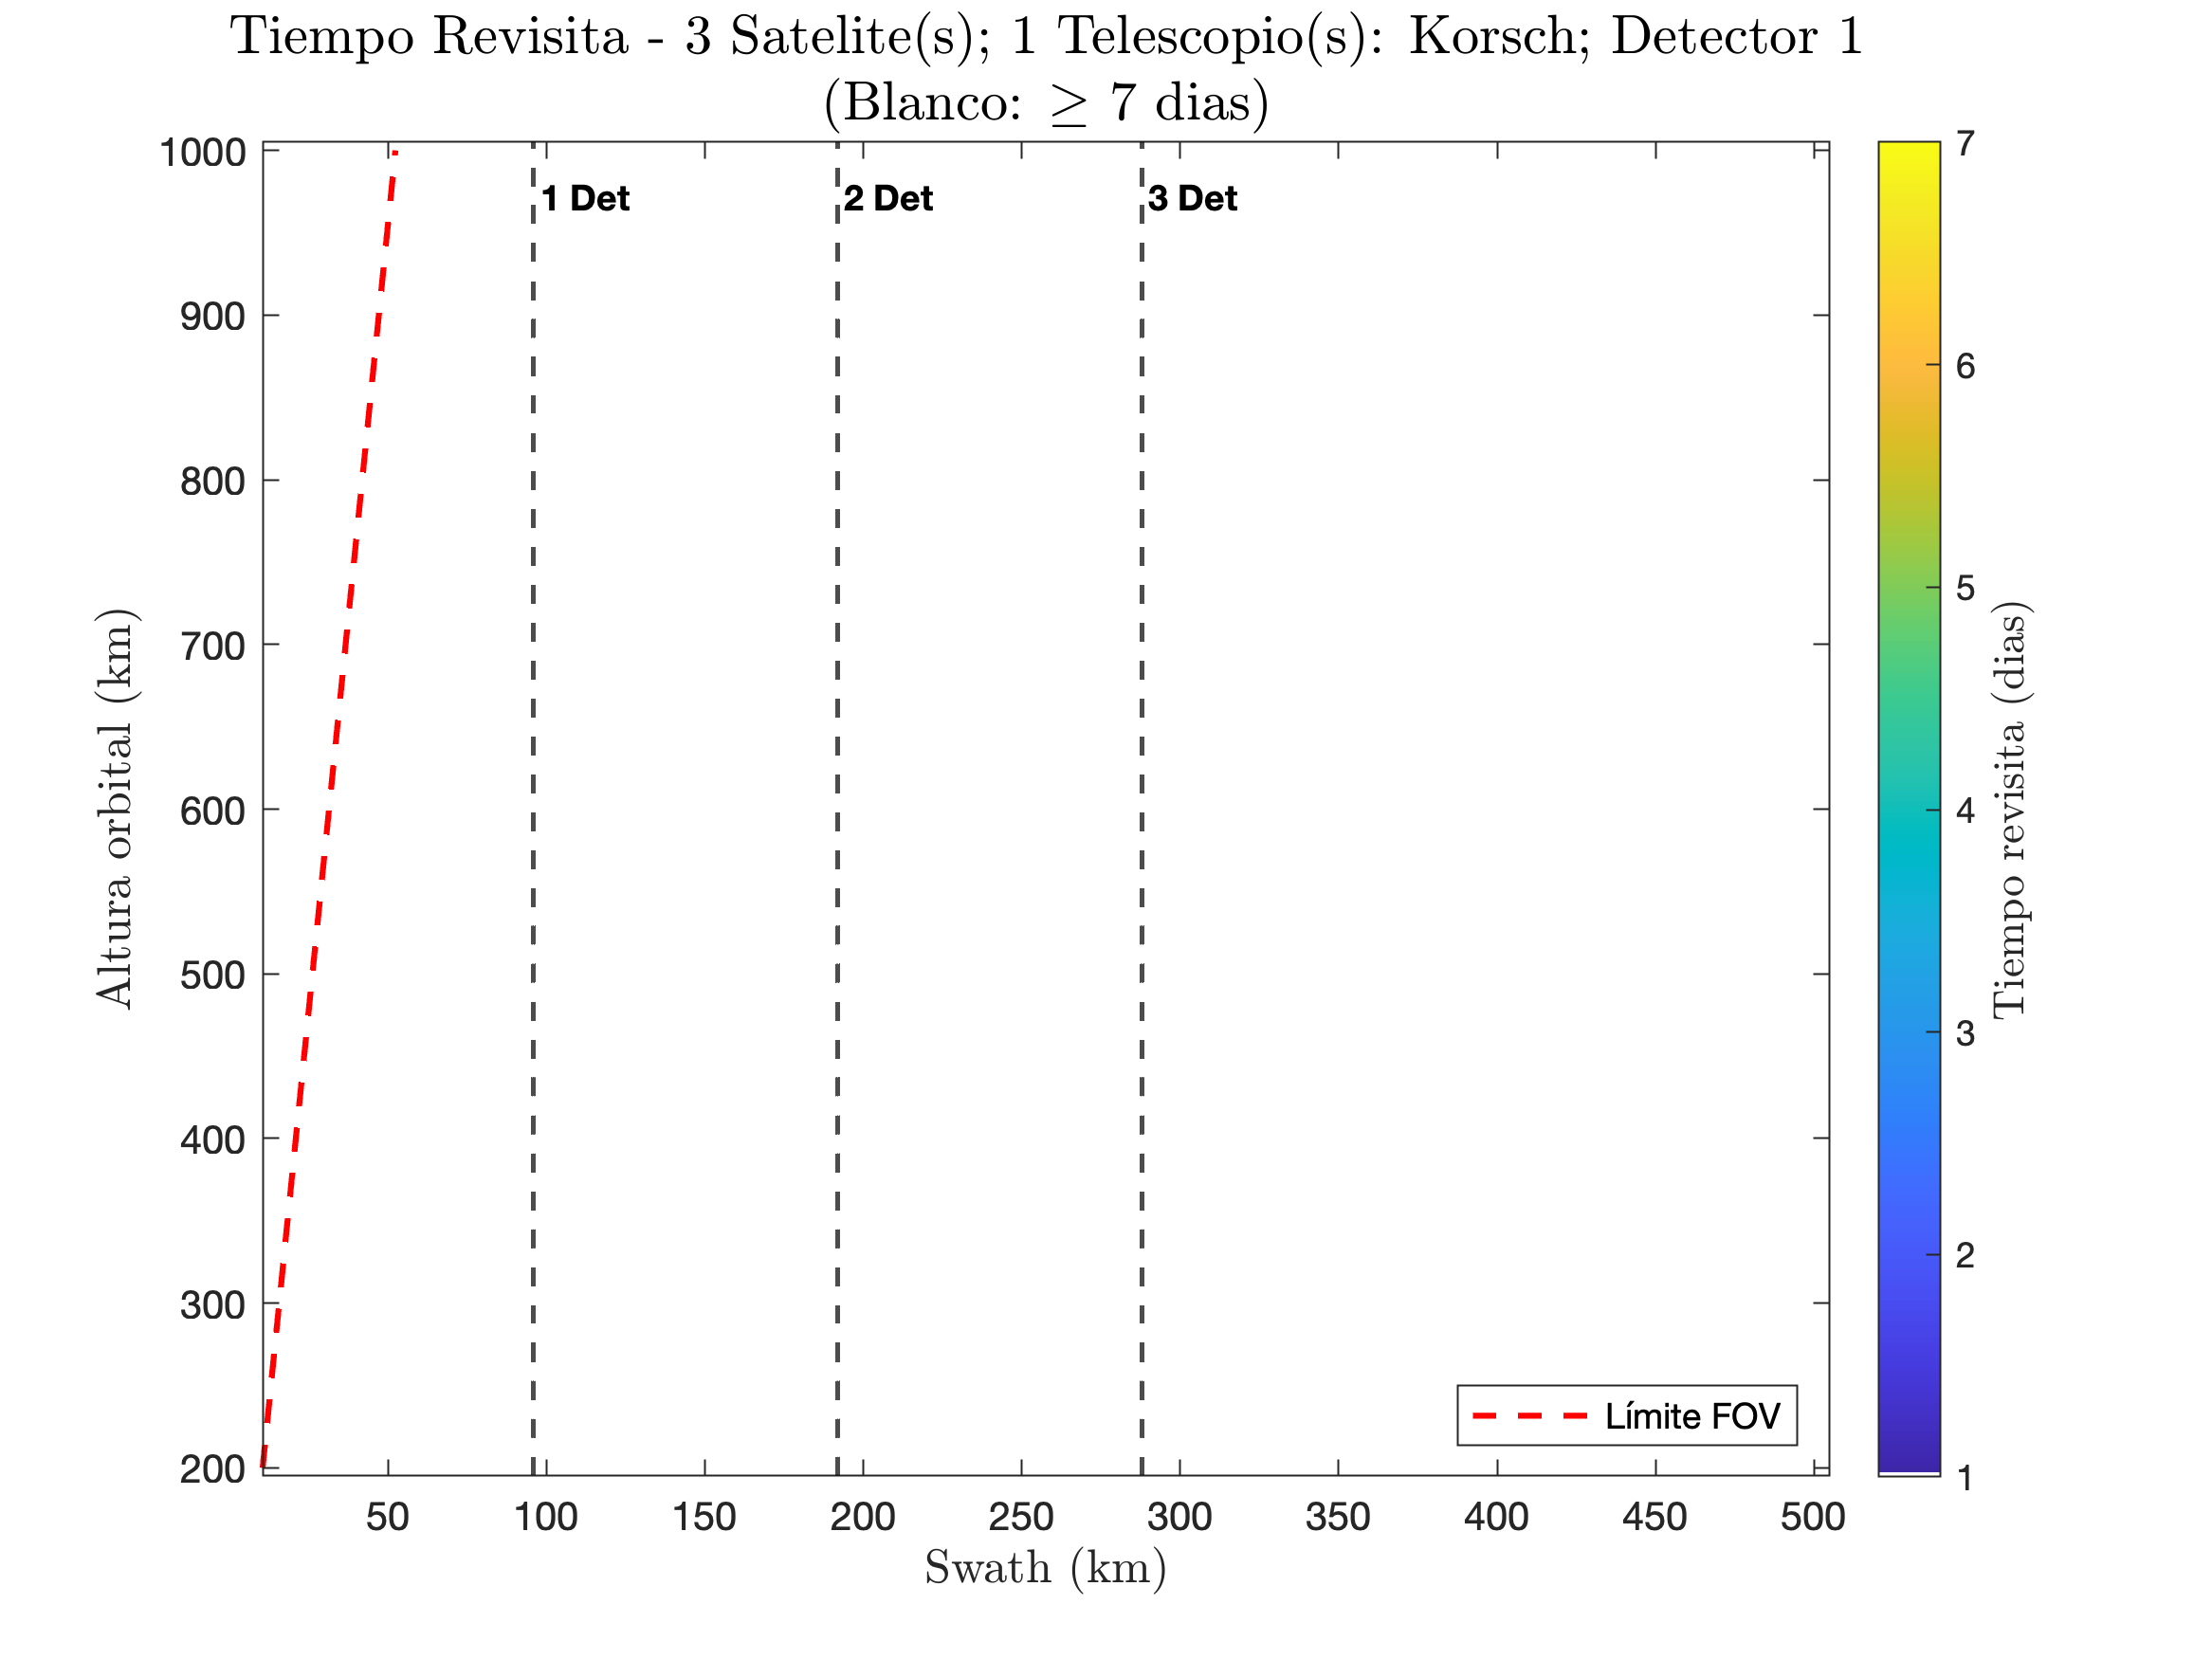
\includegraphics[width=0.48\linewidth]{4.Payload/Coverage/heatmap_3 Satelite(s); 1 Telescopio(s): Korsch; Detector 1.jpg} \\
\includegraphics[width=0.48\linewidth]{4.Payload/Coverage/heatmap_3 Satelite(s); 1 Telescopio(s): Cassegrain; Detector 1.jpg} &
\includegraphics[width=0.48\linewidth]{4.Payload/Coverage/heatmap_3 Satelite(s); 1 Telescopio(s): TMA; Detector 1.jpg} \\
\end{tabular}
\caption{Mapas de calor resultantes del cálculo de cobertura para el Detector 1, con 3 satélites.}
\end{figure}
\end{landscape}

\begin{landscape}
\begin{figure}[p]
\centering
\vspace*{0.3cm}
\setlength{\tabcolsep}{4pt}
\renewcommand{\arraystretch}{0}
\begin{tabular}{cc}
\includegraphics[width=0.48\linewidth]{4.Payload/Coverage/heatmap_3 Satelite(s); 1 Telescopio(s): Refractivo; Detector 2.jpg} &
\includegraphics[width=0.48\linewidth]{4.Payload/Coverage/heatmap_3 Satelite(s); 1 Telescopio(s): Korsch; Detector 2.jpg} \\
\includegraphics[width=0.48\linewidth]{4.Payload/Coverage/heatmap_3 Satelite(s); 1 Telescopio(s): Cassegrain; Detector 2.jpg} &
\includegraphics[width=0.48\linewidth]{4.Payload/Coverage/heatmap_3 Satelite(s); 1 Telescopio(s): TMA; Detector 2.jpg} \\
\end{tabular}
\caption{Mapas de calor resultantes del cálculo de cobertura para el Detector 2, con 3 satélites.}
\end{figure}
\end{landscape}

\begin{landscape}
\begin{figure}[p]
\centering
\vspace*{0.3cm}
\setlength{\tabcolsep}{4pt}
\renewcommand{\arraystretch}{0}
\begin{tabular}{cc}
\includegraphics[width=0.48\linewidth]{4.Payload/Coverage/heatmap_3 Satelite(s); 1 Telescopio(s): Refractivo; Detector 3.jpg} &
\includegraphics[width=0.48\linewidth]{4.Payload/Coverage/heatmap_3 Satelite(s); 1 Telescopio(s): Korsch; Detector 3.jpg} \\
\includegraphics[width=0.48\linewidth]{4.Payload/Coverage/heatmap_3 Satelite(s); 1 Telescopio(s): Cassegrain; Detector 3.jpg} &
\includegraphics[width=0.48\linewidth]{4.Payload/Coverage/heatmap_3 Satelite(s); 1 Telescopio(s): TMA; Detector 3.jpg} \\
\end{tabular}
\caption{Mapas de calor resultantes del cálculo de cobertura para el Detector 3, con 3 satélites.}
\end{figure}
\end{landscape}


De ello, se pueden extraer las siguientes consideraciones:
\begin{itemize}
    \item Los casos (i), (ii) y (iii) no generaron en la simulación en ningún caso tiempos menores a 7 días, por lo que son descartados. Consecuentemente, será necesaria una constelación de satélites para satisfacer la condición de tiempo de revisita.
    
    \item Ambos casos (iv) y (v) sí ofrecen soluciones posibles al problema. Debido al coste adicional que supone desarrollar, fabricar y validar un satélite adicional, se priorizará la solución con el menor número de satélites posibles.
    \item Los telescopios Korsch y Cassegrein, debido a su limitado ángulo de visión, deben ser descartados, pues no ofrecen soluciones viables.
\end{itemize}

En la siguiente sección, por los motivos expuestos, solo se evalúa la configuración (iv), comparando los telescopios refractivos y TMA, para los distintos detectores\footnote{En el anexo \ref{sec:annexdata}} se podrán encontrar los resultados de masa total para la configuración (v), evidenciando de igual manera mayor masa total frente a la config. (iv).


\section{Posibles soluciones. Cruce de los datos}

Para identificar las soluciones viables que satisfacen los requisitos del cliente, se ha desarrollado un \textit{script} adicional que integra los resultados de MTF, SNR y cobertura. El algoritmo determina, para cada altura orbital y configuración, el diámetro de pupila mínimo que cumple simultáneamente los requerimientos del cliente en cada banda ($MTF \geq 0,25;\ SNR \geq 400; $ tiempo de revisita $\leq 7$ días.):

%% GRAFICAS
\begin{figure}[H]
    \centering
    \includegraphics[width=1\linewidth]{4.Payload/HvsDmin_2sat_2tel.jpg}
    \caption{Comparativa del rendimiento de detectores con telescopio refractivo. \\Fuente: Elaboración propia.}
\end{figure}

A la vista de este gráfico, se puede concluir que el \textbf{telescopio refractivo} ofrece el mejor rendimiento para todas las alturas, pues el telescopio TMA necesita diámetros casi 3 veces mayores para ofrecer una solución viable, debido a su limitación de MTF. Además, el refractivo en ningún caso supera su limitación de 80 mm. Si se comparan los resultados del telescopio refractivo entre los distintos detectores:

\begin{figure}[H]
    \centering
    \includegraphics[width=1\linewidth]{4.Payload/HvsDmin_Refractivo_Config_2sat_2tel.jpg}
    \caption{Comparativa del rendimiento de detectores con telescopio refractivo. \\Fuente: Elaboración propia.}
\end{figure}

Se puede comprobar que el \textbf{detector 2: TeleDyne H2RG} ofrece el mejor rendimiento para cuales quiera de las alturas, siendo esta la opción elegida.



